%% This is file `DEMO-TUDaThesis.tex' version 4.00 (2025-01-26),
%% it is part of
%% TUDa-CI -- Corporate Design for TU Darmstadt
%% ----------------------------------------------------------------------------
%%
%% Copyright (C) 2018--2025 by Marei Peischl <marei@peitex.de>
%%
%% ============================================================================
%% This work may be distributed and/or modified under the
%% conditions of the LaTeX Project Public License, either version 1.3c
%% of this license or (at your option) any later version.
%% The latest version of this license is in
%% http://www.latex-project.org/lppl.txt
%% and version 1.3c or later is part of all distributions of LaTeX
%% version 2008/05/04 or later.
%%
%% This work has the LPPL maintenance status `maintained'.
%%
%% The current maintainer of this work is
%%   Marei Peischl <tuda-ci@peitex.de>
%%
%% The development repository can be found at
%% https://github.com/tudace/tuda_latex_templates
%% Please use the issue tracker for feedback!
%%
%% If you need a compiled version of this document, have a look at
%% http://mirror.ctan.org/macros/latex/contrib/tuda-ci/doc
%% or at the documentation directory of this package (if installed)
%% <path to your LaTeX distribution>/doc/latex/tuda-ci
%% ============================================================================
%%
% !TeX program = lualatex
%%

\RequirePackage{pdfmanagement}
\SetKeys[document/metadata]{pdfversion=1.7,pdfstandard=a-2b}
%https://github.com/tudace/tuda_latex_templates/issues/521
% Enable PDF/A via pdfmanagement and no longer via pdfx
%\DocumentMetadata{
%	pdfstandard=a-2b,
%	pdfversion=1.7,% 2.0 is possible as well, but PDF/A-2b requires < 2.0
%	lang=de,
%}

\documentclass[
	ngerman,% Main language as global option
	accentcolor=9c,% Choose accent color: For a list of available colors see the full tudapub documentation
	ruledheaders=section,% Section levels above this one will follow the ruled layout
	class=report,% Choose the base document class. Will choose the matching KOMA-Script class
	thesis={type=bachelor},% Thesis. For PhD thesis have a look at DEMO-TUDaPhd example file
	fontsize=11pt,% Basic font size. CI default setting of 9pt is too small for theses
	parskip=half-,% Use a parskip instead of indent, see KOMA-Script documentation
	custommargins=true,% Calculate margins using typearea
	marginpar=false,% Disable marginpar
%	BCOR=5mm,% Binding correction
%	accept-missing-logoes=true,% No error in case logo files are not available
%	logofile=example-image,% In case logo should be replaced
]{tudapub}


%%%%%%%%%%%%%%%%%%%
% Language setup
%%%%%%%%%%%%%%%%%%%
%\usepackage[main=english]{babel}
\usepackage[main=ngerman]{babel}
\usepackage{microtype}
\usepackage[autostyle]{csquotes}% \enquote, to simplify use of quotation marks

%%%%%%%%%%%%%%%%%%%
% Bibliography
%%%%%%%%%%%%%%%%%%%
\usepackage{biblatex}
\addbibresource{DEMO-TUDaBibliography.bib}% File name of BibTeX database

%%%%%%%%%%%%%%%%%%%
% Package suggestions for tables
%%%%%%%%%%%%%%%%%%%
\usepackage{array}% Fundamental tools for tables. Is automatically loaded by the following packages
%\usepackage{tabularx}% Tables with flexible columns to achieve fixed width
%\usepackage{longtable}% Tables across multiple pages
%\usepackage{xltabular}% Tables with fixed width spanning multiple pages
%\usepackage{booktabs}% Improved layout for horizontal rules in tables

%%%%%%%%%%%%%%%%%%%
% Package suggestions math
%%%%%%%%%%%%%%%%%%%
\usepackage{mathtools}% Extended version of amsmath
\usepackage{amssymb}% Additional symbols
%\usepackage{siunitx}% Numbers and Units

%%%%%%%%%%%%%%%%%%%
% userpackages
%%%%%%%%%%%%%%%%%%%
%\usepackage{graphicx}
\usepackage{minted}
\usepackage{pdfpages}

\hypersetup{% Metadata adjustments, in case these are not set, the data provided for \maketitle will be used
	pdfauthor=Konstantin Bachem,%Marei Peischl (peiTeX),
	pdfcreationdate=2024-05-03,
	pdfkeywords={TU Darmstadt; Corporate Design; LaTeX}
}

\title{Visualisierung des Innenprodukt-Nullraums (IPNS) von geometrischer Algebra als Iso-Oberflächen}
%\subtitle{3D-Visualisierung von Oberflächenhüllkurven an polynomialen Nullstellen mittels geometrischer Algebra}
\author{Konstantin Bachem}
\reviewer{Dr.-Ing. Dietmar Hildenbrand \and Hon.Prof. Dr.-Ing. Andr\'e Stork}

% The following elements will be placed on the title page
\department{inf}% If defined the shorthand will be replaced by the full name otherwhise it's used directly.
%\institute{}
\group{Graphisch-Interaktive Systeme}

\submissiondate{\today}
\examdate{\today}

%\tuprints{urn=XXXXX,printid=XXXX,year=2022,license=cc-by-4.0}% License information for TUprints

\begin{document}

\maketitle

%% The affidavit was deactivated by default at the request of Department II.
%% According to the department, the legally binding text can be found at https://www.tu-darmstadt.de/studieren/studierende_tu/studienorganisation_und_tucan/hilfe_und_faq/artikel_details_de_en_37824.de.jsp
%%  The docx file should be used, printed out, signed, scanned and then integrated.
%% The easiest way to do this is to use the pdfpages package.
%%
%% For compatibility reasons for the other templates, the function is still available.
%% \affidavit[signature-image={\includegraphics[width=\width,height=1cm]{example-image}}, <there may be additional options here>]

\tableofcontents
% Additional lists like \listoffigures or acronyms might be added here


%\addchap{About this file}

%\enquote{DEMO-TUDaThesis.tex} is a basic template for theses using the Corporate Design of TU Darmstadt.
%It is part of TUDa-CI, which is the official template bundle of TU Darmstadt. The original version was inspired by the \enquote{tuddesign} bundle by C.~v.~Loewenich and J.~Werner.


\includepdf{pictures/Avidavid.pdf}

\chapter{Motivation}
Geometrische Algebra hat den großen Vorteil, dass die algebraischen Ausdrücke in vielen Fällen geometrischen Objekten und Operationen entsprechen. Deshalb können Algorithmen gut visualisiert werden. Auch \textsc{Gaalop} und das web-basierte \textsc{Gaalop}Web bietet diese Möglichkeit. Insbesondere im Kontext von Algebren höherer Dimensionen, die in letzter Zeit immer wichtiger wird, weisen diese Visualisierungen allerdings eine Reihe von Nachteilen auf.
Das Ziel dieser Bachelorarbeit ist deshalb, eine neue Art der Visualisierung von geometrischen Objekten zu entwickeln und in \textsc{Gaalop}/\textsc{Gaalop}Web zu integrieren, bei der auch problemlos mit höheren Dimensionen gearbeitet werden kann. Neben der korrekten Visualisierung ist eine niedrige Laufzeit wichtig, da die Tools üblicherweise interaktiv bei der Entwicklung von Algorithmen genutzt werden.

\IMRADlabel{introduction}
\chapter{Einleitung}
%Worum geht es in dieser Arbeit? Warum das Ganze?
Geometrische Algebra ist ein mathematischer Rahmen, der viele klassische algebraische Strukturen vereinigt. Dabei entsprechen algebraische Ausdrücke geometrischen Objekten.

Aktuelle Methoden zur Visualisierung von geometrischer Algebra können nur niedrigdimensionale Algebren visualisieren oder sind langsam in höher dimensionalen Algebren.
In dieser Arbeit wird eine Methode zur schnellen Auswertung des IPNS/OPNS mittels GPU-Shadern entwickelt und darauf aufbauend Visualisierungsmethoden.



\section{Gliederung}
Die Arbeit beginnt mit einem Grundlagenkapitel, in dem relevante bekannte Algorithmen und Konzepte der Computergrafik und Mathematik vorgestellt werden. Dann folgt ein Kapitel zum Stand der Technik, in dem die aktuellen Visualisierungsmethoden vorgestellt werden.

Als Nächstes folgt ein Kapitel zur Konzeption und Anforderungen dieser Arbeit.

Dann folgen zwei Kapitel, die meine Visualisierungsansätze vorstellen. Diese sind unterteilt in auf Raycasting aufbauende Methoden und volumenbasierte Methoden, die versuchen Primitive zu erzeugen. Dann folgt ein Kapitel zur Implementierung und eingesetzten Optimierungen. Dabei wird im unter anderem ein Verfahren vorgestellt, das ermöglicht den IPNS/OPNS von höherdimensionalen Algebren auf der GPU auszuwerten.
Als Nächstes folgt ein Kapitel zur Evaluation der vorgestellten Ansätze.
Danach kommt die Zusammenfassung welche kurz die Ergebnisse der Arbeit Zusammenfasst.
Zum Schluss Kommt ein Ausblick Kapitel, in dem ich Verbesserungsideen aufzähle, die ich nicht mehr Implementieren konnte.
%Schreibe rest wenn etwas in dem entsprechenden kapitel steht.
\section{Worum geht es?}
Um ein bisschen klarer zu machen, worum es geht, gebe ich hier ein kurzes Beispiel.
Der Input von \textsc{Gaalop} sind Ausdrücke in CLUCalc. Dies ist die Sprache die \textsc{Gaalop} nutzt, um geometrische Algebra zu beschreiben. 
Dies sieht beispielsweise so aus:
\begin{verbatim}
//algebra DCGA
T1 = Toroid(R1, r1);                
Pl = Plane(nx, ny, nz, d);    
CurveTP = T1 ^ Pl; //Schnitt von Torus und Ebene                

:Blue;
:T1; //Dieser Ausdruck sagt, dass der Torus visualisiert werden soll

:Red;
:CurveTP;

:Green;
:Pl;     
\end{verbatim}
Dies wird dann mittels \textsc{Gaalop} verarbeitet und \textsc{Gaalop}s Output kann dann in meinen Visualisierer gefüttert werden.

In meiner Software wird dann der Nullraum der Objekte visualisiert.
\begin{figure}
    \centering
    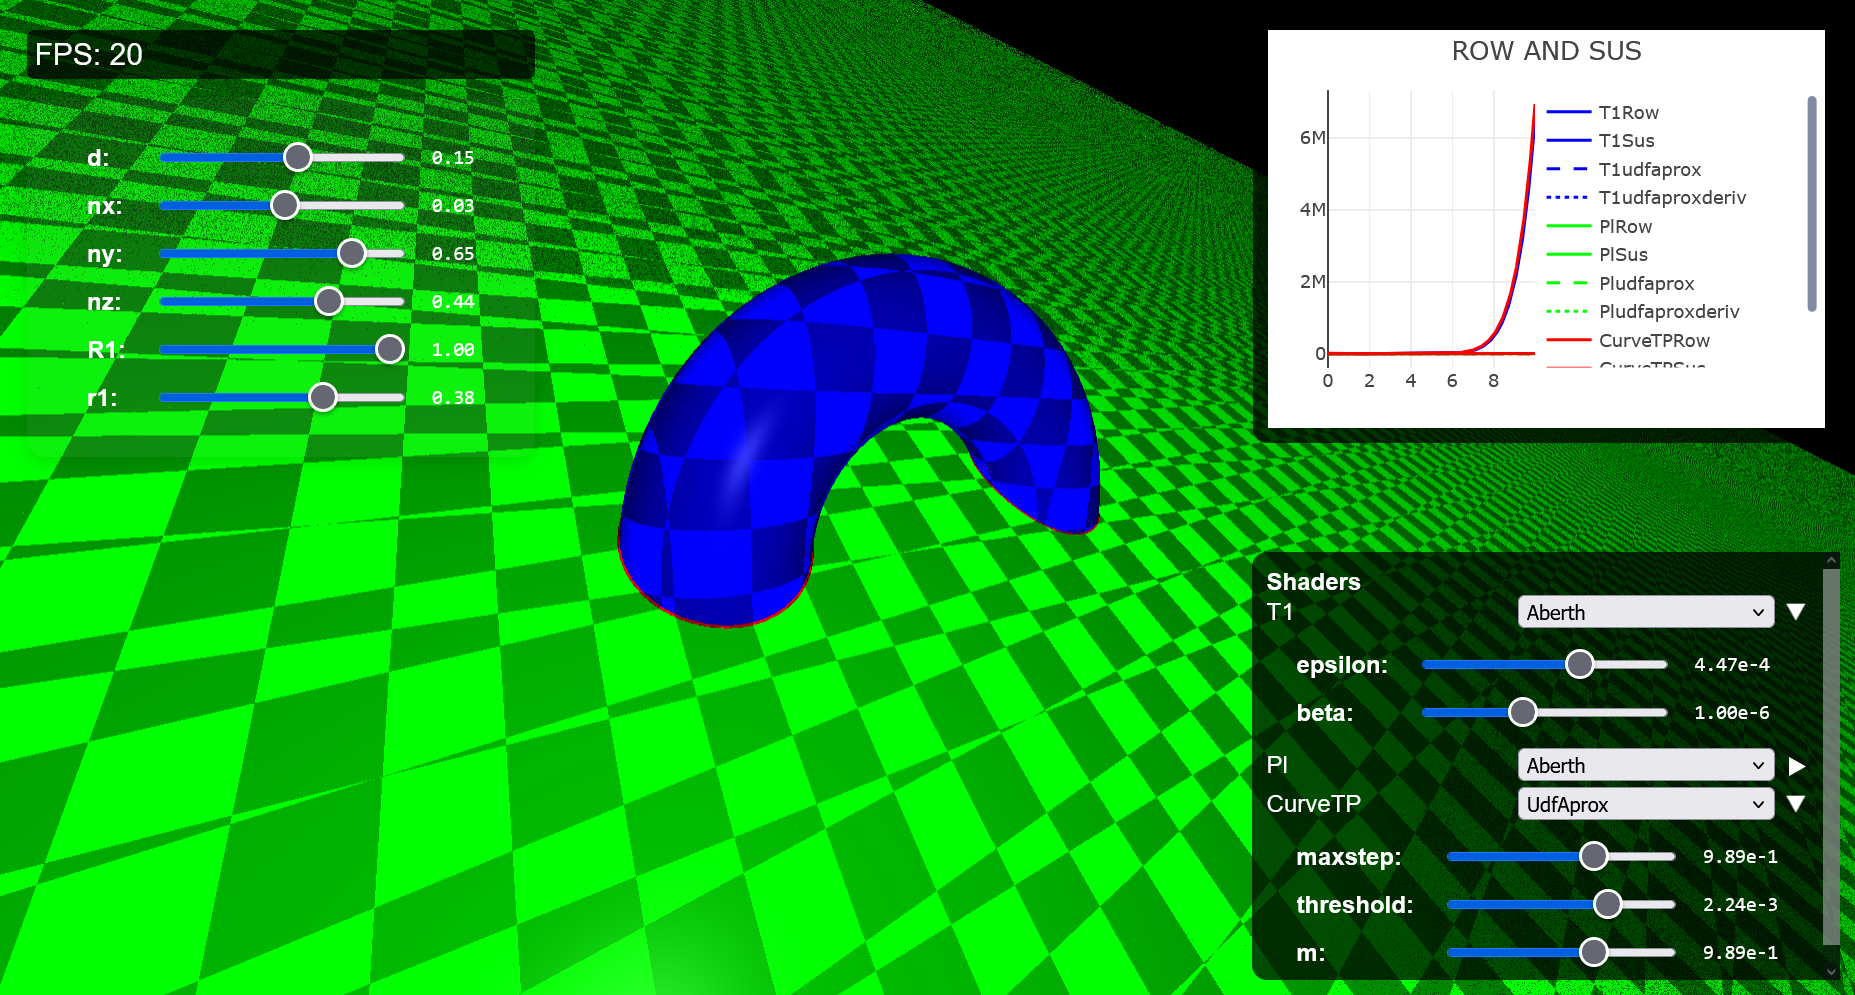
\includegraphics[width=1\linewidth]{pictures/gui.png}
    \caption{Oben links kann man mittels Schiebereglern Parameter einstellen. Oben rechts ist ein Diagramm was ich zur Debugzwecken benutzt habe. Unten rechts kann man für jedes Objekt die Visualisierungsmethode und Parameter der gewählten Methode einstellen.}

    \label{fig:gui}
\end{figure}
    

\chapter{Grundlagen}
In diesem Kapitel werden grundlegende Konzepte vorgestellt, die für das Verständnis der Arbeit wichtig sind. Zunächst wird eine kurze Einführung für geometrische Algebra gegeben. Dann wird die implizite Darstellung von Objekten der geometrischen Algebra beschrieben.
Als Nächstes werden die Grundlagen des Raycastings und der OpenGL Pipeline erklärt. Anschließend werden mehrere iterative numerische Verfahren zur Nullstellensuche vorgestellt. Und zum Schluss werden noch weitere mathematische Konzepte vorgestellt. 
Die Inhalte dieses Kapitels stammen aus der Fachliteratur und dem allgemeinen Wissensstand und wurden nicht von mir selbst entwickelt.

\section{Was ist geometrische Algebra? }

Geometrische Algebra ist ein mathematischer Rahmen, der klassische Zahlensysteme und Vektorräume zu einem einheitlichen algebraischen Konzept zusammenfasst. Viele algebraische Strukturen wie komplexe Zahlen, Quaternionen oder duale Zahlen lassen sich als spezielle geometrische Algebren konstruieren.

Geometrische Algebra wird über einem Vektorraum aufgebaut. 
Die Basisvektoren einer \( n \)-dimensionalen geometrischen Algebra werden dabei als \( e_1, \dots, e_n \) dargestellt.

\subsection{Geometrisches Produkt}
Ein zentrales Element der geometrischen Algebra ist das geometrische Produkt. Für die Basisvektoren gilt:  
\[
e_i^2 \in \{ -1, 0, 1 \}
\]

Welche dieser Werte tatsächlich auftreten, hängt dabei von der Signatur der zugrunde liegenden Algebra ab.

Die Schreibweise \( \mathcal{G}_{3,1,0} \) steht beispielsweise für eine geometrische Algebra mit Signatur \((3,1,0)\):  
Die ersten drei Basisvektoren quadrieren zu \( +1 \), der vierte zu \( -1 \), und keiner zu \( 0 \).

Eine weitere Eigenschaft ist:  
\[
e_i e_j = - e_j e_i \quad \text{für } i \neq j.
\]
Das Produkt \( e_i e_j \) ist dabei weder eine reelle Zahl noch ein Element des ursprünglichen Vektorraums. Stattdessen entsteht ein neues Objekt: ein sogenannter \textbf{Blade}.

Blades sind die grundlegenden Bausteine der geometrischen Algebra. Für eine Algebra mit \( n \) Basisvektoren gibt es \( 2^n \) Blades. \\
Beispielsweise gibt es für die Basis \( e_1, e_2, e_3 \) insgesamt 8 Blades:

\begin{itemize}
    \item Basisvektoren: \( e_1, e_2, e_3 \)
    \item 2-Blades : \( e_1 \wedge e_2, e_1 \wedge e_3, e_2 \wedge e_3 \)
    \item 3-Blade : \( e_1 \wedge e_2 \wedge e_3 \)
\end{itemize}

Die Kurzschreibweise \( e_{12} \coloneqq e_1 \wedge e_2 \) wird häufig verwendet, um Blades kompakt \\
darzustellen.

Linearkombinationen der Basisvektoren werden Vektoren genannt. Analog dazu werden Linearkombinationen von 2-Blades Bivektoren und Linearkombinationen von 3-Blades Trivektoren genannt usw. 
Weiterhin werden Linearkombinationen beliebiger Blades Multivektoren genannt. Diese bilden die Objekte der geometrischen Algebra.

\subsection{Inneres und äußeres Produkt}
Das geometrische Produkt zweier Vektoren \(u, v\) kann in das innere (\(u \cdot v\)) und das äußere (\(u \wedge v\)) Produkt zerlegt werden.

Seien
\[
u = u_x e_1 + u_y e_2 + u_z e_3, \quad
v = v_x e_1 + v_y e_2 + v_z e_3
\]

Dann gilt:
\[
uv = u \cdot v + u \wedge v
\]
wobei (unter der Annahme, dass \((e_{1})^2=(e_{2})^2=(e_{3})^2=1\))
\[
u \cdot v = u_x v_x + u_y v_y + u_z v_z
\]
und
\[
u \wedge v =
(u_x v_y - u_y v_x)\, e_{12}
+ (u_z v_x - u_x v_z)\, e_{31}
+ (u_y v_z - u_z v_y)\, e_{23}
\]

Das innere Produkt entspricht in diesem Fall also dem Skalarprodukt und das äußere dem Kreuzprodukt.
Dabei ist das innere Produkt symmetrisch (das heißt
\(u \cdot v = v \cdot u\)),
während das äußere Produkt antisymmetrisch ist
(\(u \wedge v = - v \wedge u.\))
Diese Zerlegung und Eigenschaften gelten jedoch nur für Vektoren.

\subsection{Produkt zweier Multivektoren}
Durch Anwendung der Axiome kann man Produkte beliebiger Basis-Blades berechnen. Beispielsweise (unter der Annahme, dass \((e_{1})^2=(e_{2})^2=1\)): 
\[
(e_{12})^2 = (e_1 \wedge e_2)(e_1 \wedge e_2) = e_1 (e_2 e_1) e_2 = - e_1 e_1 e_2 e_2 = -1
\]
Dies ergibt sich durch Anwendung der Antisymmetrie und Assoziativität des geometrischen Produkts.

Um Produkte von zwei Multivektoren in der Praxis zu berechnen, werden sogenannte Cayley-Tabellen genutzt.
Diese sind einfach Lookup-Tabellen für die Produkte der Basis-Blades.


%bild

Zwei Multivektoren 
\[
A = \sum_I a_I e_I, \quad B = \sum_J b_J e_J,
\]
können dann folgendermaßen multipliziert werden:
\[
AB = \sum_{I,J} a_I b_J (e_I e_J),
\]

Wobei das Produkt \(e_I e_J\) direkt aus der Cayley-Tabelle abgelesen wird.
Analog kann das gleiche für das innere und äußere Produkt gemacht werden mit jeweils eigenen Cayley-Tabellen.



\subsection{Produkt als Matrix}
%Das chapter ist unverständlich

Man kann Produkte von zwei Multivektoren auch als Matrix-Vektor-Produkt darstellen. 
Dabei wird ein Multivektor in eine Matrix umgewandelt, während der andere in den Vektor umgewandelt wird. Dies ermöglicht eine einfache Berechnung von dem als Matrix dargestellten Multivektor mit beliebigen anderen Multivektoren.


Ein Multivektor-Produkt in Code sieht ungefähr so aus:

\begin{minted}{python}
def product(A, B, table):
    result = defaultdict(int)
    for coeffA, bladeA in A.items():
        for coeffB, bladeB in B.items():
            sign, bladeO = table[bladeA, bladeB]
            result[bladeO] += sign * coeffA * coeffB
    return result
\end{minted}

Für die Umwandlung in eine Matrixform, wobei der linke Faktor \( A \) fest ist:

\begin{minted}{python}
def toMatrix(A, table):
    matrix = defaultdict(int)
    for coeffA, bladeA in A.items():
        for bladeB in allBlades:
            sign, bladeO = table[bladeA, bladeB]
            matrix[bladeO, bladeB] = sign * coeffA
    return matrix
\end{minted}

Diese Matrix kann nun als lineare Abbildung auf beliebige rechte Faktoren \( B \) angewendet werden, wobei die Multiplikation \( A \cdot B \) als gewöhnliches Matrix-Vektor-Produkt umgesetzt wird.

\begin{minted}{python}
def applyMatrix(matrix, B):
    result = defaultdict(int)
    for row in allBlades:
        for col, coeffB in B.items():
            result[row] += matrix[row, col] * coeffB
    return result
\end{minted}

Ich habe hier die Matrix, die Multivektoren und die Cayley-Tabelle der Übersichtlichkeit halber als Dictionary repräsentiert. Allerdings könnte man natürlich auch gewöhnliche Arrays verwenden.

%\chapter{Grundlagen}

\section{Implizite Darstellung}
\subsection{Implizite Funktionen}
Eine Möglichkeit, um geometrische Objekte in 3D zu repräsentieren, sind implizite
Gleichungen der Form:
\[
f(x, y, z) = c
\]

Alle Punkte $(x, y, z)$, welche diese Bedingung erfüllen, bilden zusammen im Raum eine Fläche
(oder Kurve bzw. Punktmenge). Diese Repräsentation wird auch Isofläche genannt. Zur
Vereinfachung verwende ich stets $c = 0$. Ein Beispiel für die Repräsentation einer Kugel ist:
\[
(x - c_x)^2 + (y - c_y)^2 + (z - c_z)^2 - r^2 = 0
\]

Hierbei ist $c$ der Mittelpunkt der Kugel und $r$ der Radius.



\subsection{Signed Distance Functions (SDF)}
Eine Signed Distance Function (SDF) ist eine spezielle Isofläche, welche die kleinste
euklidische Distanz zu einem Objekt beschreibt. Sie ist innerhalb des Objektes positiv und
außerhalb negativ (oder umgekehrt, je nach Konvention) und auf dem Objekt $0$.

Ein Beispiel für die SDF einer Kugel ist:
\[
\sqrt{(x - c_x)^2 + (y - c_y)^2 + (z - c_z)^2} - r = 0
\]

Für SDFs gibt es mehrere einfache und schnelle Methoden zur Visualisierung.




\subsection{Unsigned Distance Functions (UDF)}
Unsigned Distance Functions (UDF) sind ähnlich zu SDFs, mit dem einzigen Unterschied,
dass sie immer positiv sind. Dieser Unterschied macht das Detektieren einer Nullstelle
schwerer, da es keinen Nulldurchgang gibt. Stattdessen muss ein Schwellwert hinzugefügt
werden, welcher entscheidet, ob eine Nullstelle erreicht ist.

\subsection{IPNS/OPNS}
Um ein Objekt \texttt{obj} in der Geometrischen Algebra als Isofläche darzustellen, wird der sogenannte IPNS und OPNS (Inner/Outer Product Null Space) verwendet. Dieser stellt Objekte der geometrischen Algebra als eine implizite Darstellung dar.

Für OPNS gilt:
\[
\text{point}(x,y,z) \wedge \texttt{obj} = 0
\]

Für IPNS gilt entsprechend:
\[
\text{point}(x,y,z) \cdot \texttt{obj} = 0 
\]

\text{point}, das innere und das äußere Produkt sind dabei abhängig von der Algebra. Die Funktion \(\text{point}(x, y, z)\) erzeugt dabei einen Punkt in der Algebra und wird unter anderem auch als \enquote{up} bezeichnet.

Statt die Ergebnisse dieser Produkte als Multivektoren zu interpretieren, 
kann man sie auch als konventionelle vektorwertige Funktion
\[
F : \mathbb{R}^3 \to \mathbb{R}^n, 
\quad (x,y,z) \mapsto \mathbf{F}(x,y,z)
\]
auffassen.

Dabei besteht F aus den Koeffizienten von \(
\text{point}(x,y,z) \wedge \texttt{obj}
\)
bzw.
\(
\text{point}(x,y,z) \cdot \texttt{obj}
\).






\subsubsection{F als Skalar}
Um das Ergebnis von \( \mathbf{F}(x,y,z) \) zu einem Skalar zu überführen, wird die Summe der Quadrate verwendet:
\[
f(x,y,z) = \|\mathbf{F}(x,y,z)\|^2
\]

Da \( f(x,y,z) \) die quadrierte Euklidische Norm von \( \mathbf{F}(x,y,z) \) ist, gilt:
\[
\mathbf{F}(x,y,z) = 0 \quad \Leftrightarrow \quad f(x,y,z) = 0
\]

Die Arbeit mit \( f \) ist in vielen Fällen einfacher als mit \( \mathbf{F} \), da das ursprüngliche vektorwertige Problem auf die Bestimmung der Nullstellen einer skalarwertigen Funktion reduziert wird. Auch Ganja und \textsc{Gaalop} nutzen die Summe der Quadrate zur Visualisierung.


Da $f$ die Summe der Quadrate von \( \mathbf{F} \) ist, ist $f \geq 0$ für alle $x,y,z$. Es handelt sich also nicht um eine Distanzfunktion im klassischen Sinne. $f$ ist weder eine SDF noch eine UDF. 

Ein Nachteil der skalarisierten Darstellung ist, dass \( f \) ein Polynom ist, dessen Grad durch das Quadrieren der Terme in \( \mathbf{F} \) verdoppelt wird. 

Zum Beispiel enthält \( \mathbf{F} \) in der DCGA (Double Conformal Geometric Algebra) Polynome vierten Grades, sodass \( f \) in diesem Fall ein Polynom bis zum achten Grad sein kann.

\section{Raycasting}
\subsection{OpenGL-Pipeline}

Ein OpenGL-Programm besteht normalerweise aus einem Vertex-Shader und einem Fragment-Shader.
Die Inputdaten für die GPU-Pipeline sind normalerweise grafische Primitive wie zum Beispiel Dreiecke. 

Die erste Stufe der Pipeline ist der Vertex-Shader. Dieser manipuliert die Vertices (also Eckpunkte) der Primitive. Beispielsweise transformiert er die Eckpunkte von Dreiecken mit einer Kameramatrix. 

Die nächsten wichtigen Stufen sind Primitive Assembly und Rasterization. Dabei werden die Dreiecke (oder andere Primitive) auf den Bildschirm projiziert und zu Fragmenten umgewandelt. Für jedes Pixel, den ein Dreieck auf dem Bildschirm überdeckt, wird ein Fragment erzeugt. 

Diese Fragmente werden in der nächsten Stufe, dem Fragment-Shader, verarbeitet. Dort wird für jedes Fragment die endgültige Farbe berechnet, sowie gegebenenfalls die Tiefe (Z-Wert) für das Depth-Buffering. Nachdem alle Fragmente eines Bildes verarbeitet wurden, werden sie gemäß Tiefe- und Transparenzregeln zusammengeführt, und das Ergebnis wird als Pixel gespeichert.

\subsection{Was ist Raycasting? }

Die Visualisierungsmethoden für geometrische Objekte auf der GPU basieren in dieser Arbeit auf Raycasting.
Beim Raycasting besteht der Input für die Pipeline aus zwei Dreiecke, die den gesamten Bildschirm abdecken. Der Vertex-Shader wird nicht wirklich benutzt. Da er allerdings angegeben werden muss, ist er einfach ein Programm, das die Vertices unverändert weitergibt. Die eigentliche Arbeit beim Raycasting passiert im Fragment-Shader. Die beiden bildschirmfüllenden Dreiecke erzeugen für jedes Pixel auf dem Bildschirm ein Fragment. Der Fragment-Shader wird also dazu genutzt, um für jedes Pixel anhand seiner Position auf dem Bildschirm seine Farbe zu berechnen.

Beim Raycasting wird für jedes Pixel ein Strahl generiert. In dieser Arbeit habe ich perspektivische
Projektion benutzt, was bedeutet, dass für jedes Pixel auf der Projektionsebene ein Strahl
vom Projektionszentrum (der Kamera) aus generiert wird. Dieser trifft dann ein Objekt (oder
den Hintergrund), und entsprechend wird dem Pixel eine Farbe zugeordnet.


%Bild https://commons.wikimedia.org/wiki/File:Ray_trace_diagram.svg
Um ein Objekt zu visualisieren, muss also der erste Schnittpunkt zwischen dem Strahl und
unserem Objekt berechnet werden.
Der Strahl wird beschrieben durch:
\[\mathbf{ray}(t)= \mathbf{r}_o + t \cdot \mathbf{r}_d \]
wobei $\mathbf{r}_o$ der Ursprung des Strahls (ray origin) und $\mathbf{r}_d$ die Richtung (ray direction) ist. Zur
Vereinfachung wird $ \mathbf{r}_d$ normalisiert (d.h. $|\mathbf{r}_d|=1$). Dies hat den Vorteil, dass ein Punkt $ p=\mathbf{ray}(t) $
genau um $t$ von der Kamera entfernt ist. Da wir einen Strahl haben, muss zusätzlich $t>0$
gelten.
    
Die implizite Funktion wird als $f(x, y, z) = 0$ beschrieben. Damit ein Punkt $p = \mathbf{ray}(t)$ in $f$ liegt,
muss also gelten:
\[
f(p) = f_{\text{ray}}(t) = 0
\]

Gefordert ist zusätzlich der erste Schnittpunkt, was bedeutet, dass das kleinste $t$ gesucht
wird, für das die anderen Bedingungen erfüllt sind.

Gesucht ist also das kleinste $t$, für das gilt: $t > 0$ und $f_{\text{ray}}(t) = 0$.

%Um dieses t zu finden, habe ich mehrere iterative Verfahren getestet.
%Die meisten Verfahren habe ich auf der shadertoy gefunden
\subsection{Spheretracing}
\label{sec:Spheretracing}
Eine der am häufigsten verwendeten Methoden zur Darstellung von UDFs und SDFs ist das Sphere Tracing.  
Der Pseudocode dazu sieht wie folgt aus:

\begin{minted}{python}
t = 0
for i in range(maxiter):
    step = UDF(ray(t))
    if step < threshold:
        return t
    t += min(step,maxstep)
return t
\end{minted}

Der \enquote{maxstep} ist dabei nicht teil des ursprünglichen Verfahrens. Allerdings benutze ich in dieser Arbeit Approximationen für die UDF die durch eine maximale Schrittweite wesentlich stabiler werden.


Diese Methode funktioniert, da für einen Punkt \( \mathbf{p} = \mathbf{ray}(t) \) die Entfernung zum Objekt mindestens  
\( d = \text{UDF}(\mathbf{p}) \) beträgt. Das bedeutet, man kann sich von \( \mathbf{p} \) aus um eine Distanz \( d \) entlang des Strahls weiterbewegen, ohne das Objekt zu treffen.

\begin{figure}
    \centering
    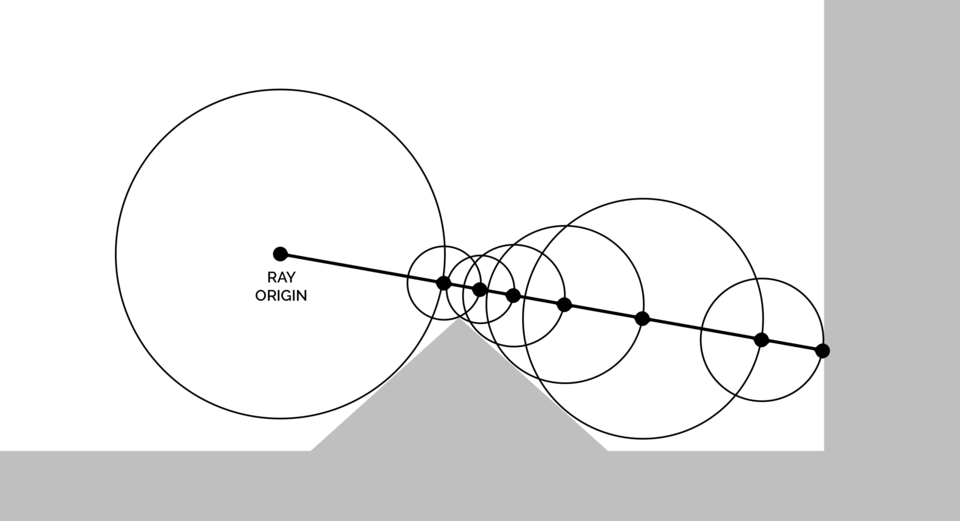
\includegraphics[width=1\linewidth]{pictures/Visualization_of_SDF_ray_marching_algorithm.png}
    \caption{Auf diesem Bild sieht man wie mittels Spheretracing der Schnitt eines Strahls mit einem Objekt gefunden werden kann. Die Kreise repräsentieren dabei die SDF/UDF. \cite{teadrinker2022sdf}}

    \label{fig:raymarch}
\end{figure}

    
\section{Verfahren zur Nullstellensuche}
\subsection{Newtonverfahren}
Das Newtonverfahren ist ein iteratives Verfahren zur Suche von Nullstellen einer Funktion. 
Die Iterationsvorschrift lautet dabei:
\[x^\text{neu}=x-\frac{f(x)}{f'(x)}\]

Ist die Multiplizität \(m\) der gesuchten Nullstelle bekannt, kann die Konvergenzgeschwindigkeit durch eine angepasste Iteration verbessert werden. In diesem Fall ergibt sich:
\[x^\text{neu}=x-m \cdot \frac{f(x)}{f'(x)}\]


\subsection{Aberth-Verfahren}
Das Aberth-Verfahren ist ein Verfahren zur Suche der komplexen Nullstellen von Polynomen. 
Im Gegensatz zum Newtonverfahren findet es alle Nullstellen gleichzeitig.

Es basiert auf folgender Formel:
\[
G_k(x) = \frac{p(x)}{\prod_{j=1;\,j\neq k}^n (x - z_j)}
\]

Dabei ist \( p \) das gegebene Polynom, und \( z_k \) sind die Näherungen an die Nullstellen. Das Polynom \( p \) wird durch alle Nullstellen außer \( z_k \) geteilt, wodurch ein neuer Ausdruck entsteht, der in der Nähe von \( z_k \) eine Nullstelle besitzt. Mittels eines Newton-Schritts wird \( z_k \) dann aktualisiert.

Die Update-Formel für den Newton-Schritt lautet:
\[
z_k^{\text{neu}} = z_k-\frac{G_k(z_k)}{G_k'(z_k)}= z_k - \frac{\frac{p(z_k)}{p'(z_k)}}{  1 - \frac{p(z_k)}{p'(z_k)} \sum_{j=1;\,j \neq k}^n \frac{1}{z_k - z_j} }
\]

Da die Nullstellen von \( f_{\text{ray}}(t) \) gesucht werden, ist \( p(t) = f_{\text{ray}}(t) \). Mit diesem Verfahren werden die Nullstellen iterativ angepasst, bis alle \( z_k \) konvergiert sind.

Als Konvergenzkriterium wird üblicherweise die maximale Änderung der Nullstellen zwischen zwei Iterationen verwendet:
\[
\max_k \left| z_k^{\text{neu}} - z_k^{\text{alt}} \right| < \varepsilon
\]

\subsection{Intervall Arithmetik}
Intervallarithmetik ist eine Methode zur sicheren Berechnung von Fehlergrenzen in numerischen Algorithmen. 
Statt mit exakten Werten zu rechnen, wird, wie der Name schon sagt, mit Intervallen gerechnet. 
Das Hauptaugenmerk bei der Intervallarithmetik liegt darin, obere und untere Schranken für den Wertebereich einer Funktion in einer oder mehreren Variablen zu bestimmen.

Beispielsweise haben wir zwei Variablen $x \in [x_1,x_2]$ und $y \in [y_1,y_2]$. $x+y$ muss also im Intervall $[x_1+y_1,x_2+y_2]$ sein.
Das Ganze kann so geschrieben werden:
\[
[x_1,x_2]+[y_1,y_2]=[x_1+y_1,x_2+y_2]
\]

Intervallarithmetik funktioniert natürlich auch für andere Operationen. Hier sind die wichtigsten:
\[
[x_1,x_2]-[y_1,y_2]=[x_1-y_2,x_2-y_1]
\]

\[
[x_1,x_2] \cdot [y_1,y_2]=[\min(x_1 y_1,x_2 y_1,x_1 y_2,x_2 y_2),\max(x_1 y_1,x_2 y_1,x_1 y_2,x_2 y_2)]
\]

\[
[x_1,x_2]^2 = 
\begin{cases} 
[0, \max(x_1^2, x_2^2)] & \text{falls } 0 \in [x_1,x_2] \\
[\min(x_1^2, x_2^2), \max(x_1^2, x_2^2)] & \text{sonst}
\end{cases}
\]

Allerdings Division nicht, da diese unstetig ist:
\[
1/[-1,1] = [-\infty,1] \cup [1,\infty]
\]
Division hätte mehrere Output-Intervalle, was nicht unterstützt wird. Um es auf ein Intervall zu bringen, müsste man $1/[-1,1] = [-\infty,\infty]$ benutzen, was nicht hilfreich ist. Für meine Anwendung ist dies jedoch kein Problem, da ich nur Division durch skalare (nicht durch Intervalle) nutze.

Man kann diese Operationen nun verketten, um komplexere Funktionen darzustellen. 
Dabei gilt in der Regel, je größer die Eingabeintervalle sind, desto ungenauer wird das Ergebnis.


Um zu bestimmen, ob eine Funktion $f(x,y,z)$ in einem 3-dimensionalen Intervall eine Nullstelle hat, kann die Funktion über den Intervallen ausgewertet werden, und es kann geprüft werden, ob $0$ in dem Ergebnis liegt.

Sei:
\[
I_x = [x_{\text{low}}, x_{\text{high}}], \quad
I_y = [y_{\text{low}}, y_{\text{high}}], \quad
I_z = [z_{\text{low}}, z_{\text{high}}], \quad
I_x, I_y, I_z \subset \mathbb{R}.
\]
Es gilt:
\[
 (\exists x \in I_x,y \in I_y,z \in I_z: f(x,y,z)=0)  \implies  0 \in f(I_x,I_y,I_z)  
\]
%\[
% (\exists (x, y, z) \in I_x \times I_y \times I_z: f(x,y,z)=0)  \implies  0 \in %f(I_x,I_y,I_z)  
%\]

Allerdings gilt die Implikation nicht umgekehrt. Es kann also nicht gezeigt werden, dass eine Funktion über einem Intervall eine Nullstelle besitzt, sondern nur, dass sie keine Nullstelle besitzt:
\[
   0 \notin f(I_x,I_y,I_z) \implies (\neg\exists x \in I_x,y \in I_y,z \in I_z: f(x,y,z)=0)  
\]

Eine Möglichkeit, dennoch näherungsweise zu zeigen, 
dass \( f \) eine Nullstelle auf dem Intervall hat, besteht darin, 
die Intervalle \( I_x, I_y, I_z \) schrittweise zu unterteilen, 
bis sie klein genug sind.

\subsection{Gauß-Newton-Verfahren}
Das Gauß-Newton-Verfahren ist ein iteratives Optimierungsverfahren für die Suche des Minimums der Summe der Quadrate einer mehrwertigen Funktion.
\[
\min _{x\in \mathbb {R} ^{n}}\left\{{\frac {1}{2}}\sum _{i=1}^{m}\left(f_{i}(\mathbf{x})\right)^{2}\right\}
\]

Der Update-Schritt für dieses Verfahren ist:
\[
\mathbf{x}^{\text{neu}} = \mathbf{x} - \alpha \left( J(\mathbf{x})^\top J(\mathbf{x}) \right)^{-1} J(\mathbf{x})^\top \mathbf{F}(\mathbf{x}),
\]
wobei $J(\mathbf{x})$ die Jacobi-Matrix der Vektorfunktion $\mathbf{F}$ an der Stelle~$\mathbf{x}$ bezeichnet und $\alpha \in \mathbb{R}$ eine Schrittweite ist.



Eine Erweiterung des Verfahrens ist:
\[\mathbf{x}^\text{neu} = \mathbf{x} - \alpha \left(J^\top J + \beta I\right)^{-1} J^\top f(\mathbf{x})\]

Dabei sorgt \(\beta I\) dafür das \(J^\top J+\beta I\) invertierbar ist.
Dies ist eine Variante des Levenberg-Marquardt-Iterationsschritts.



\section{Vandermonde-Matrix}
\label{sec:Vandermonde}
Eine einfache Möglichkeit zur Bestimmung der Koeffizienten eines Polynoms \(f\) besteht in der Verwendung einer Vandermonde-Matrix~$V$. Gegeben seien $n$ Stützstellen $x_1, x_2, \dotsc, x_n$ sowie die zugehörigen Funktionswerte $y_i=f_\text{ray}(\mathbf{ray}(x_i))$. Dann ergibt sich das Gleichungssystem
\[
V \cdot \mathbf{c} = \mathbf{y},
\]
wobei
\[
V = 
\begin{pmatrix}
1 & x_1 & x_1^2 & \cdots & x_1^{n-1} \\
1 & x_2 & x_2^2 & \cdots & x_2^{n-1} \\
\vdots & \vdots & \vdots & \ddots & \vdots \\
1 & x_n & x_n^2 & \cdots & x_n^{n-1}
\end{pmatrix},
\quad
\mathbf{c} = 
\begin{pmatrix}
c_0 \\ c_1 \\ \vdots \\ c_{n-1}
\end{pmatrix},
\quad
\mathbf{y} = 
\begin{pmatrix}
y_1 \\ y_2 \\ \vdots \\ y_n
\end{pmatrix}.
\]
Löst man dieses Gleichungssystem durch Invertieren der Matrix $V$, so ergeben sich die Koeffizienten $\mathbf{c}$ und die dazugehörige Approximation.
\[
\mathbf{c} = V^{-1} \cdot \mathbf{y},\quad f_\text{ray}(x)=\sum_{i=0}^{n-1}{c_ix^i}
\]

Die Inverse $V^{-1}$ kann dabei vorab berechnet werden, solange sich die Stützstellen $x_i$ nicht ändern.
Das bedeutet, es wird nur noch das Auswerten von \(f\) an \(\deg(f) + 1\) Stützstellen und eine Matrixmultiplikation benötigt, um die Koeffizienten zu erhalten.

\section{Duale Zahlen}
Duale Zahlen (nicht zu verwechseln zu Zahlen im Dualsystem) sind ein einfacher Weg um Ableitungen zu berechnen.
Sie definieren ähnlich zu den komplexen Zahlen eine nicht reelle Einheit \(\varepsilon\) mit der Eigenschaft \(\varepsilon^2=0\).
Daraus ergeben sich wie auch bei den komplexen Zahlen die entsprechenden Rechenregeln.
Beispielsweise erhält man durch einfaches Ausmultiplizieren die Regeln für Multiplikation:
\[(a + b \varepsilon)\cdot( c+ d \varepsilon)=a c + (a d + b c)\varepsilon + b d \varepsilon^2 =a c + (a d + b c)\varepsilon\]

Es gilt: \[f(x+\varepsilon)=f(x)+f'(x)\varepsilon\]

Duale Zahlen realisieren Forward-Mode Automatic Differentiation.
Diese Ableitungstechnik eignet sich insbesondere dann, wenn die abzuleitende Funktion mehr Ausgaben als Eingaben besitzt.
Im Gegensatz dazu steht die Backpropagation (Reverse-Mode Automatic Differentiation), die bevorzugt verwendet wird, wenn die Funktion mehr Eingaben als Ausgaben hat.

Um duale Zahlen auf mehrere Inputs zu erweitern, müssen mehrere \(\varepsilon_i\) eingeführt werden mit der Eigenschaft \(\forall i,j: \varepsilon_i\varepsilon_j=0\).


Es gilt:
\[
f(x+\varepsilon_1,\; y+\varepsilon_2,\; z+\varepsilon_3)
=
f(x,y,z)
+ \frac{\partial f(x,y,z)}{\partial x}\,\varepsilon_1
+ \frac{\partial f(x,y,z)}{\partial y}\,\varepsilon_2
+ \frac{\partial f(x,y,z)}{\partial z}\,\varepsilon_3.
\]

\chapter{Stand der Technik}
In diesem kapitel werde ich \textsc{Gaalop}s und Ganjas Visualisierungsansätze vorstellen. Auf diesen ansätze bauen meine ansätze weitgehend auf. Außerdem werde ich noch einen dritten Ansatz vorstellen.
\section{Ganja}
Ganja \cite{ganja} ist eine Library für geometrische Algebra die von vielen anderen Libraries zur Visualisierung benutzt wird. Auch \textsc{Gaalop}Web nutz Ganja zur Visualisierung.
Dabei benutzt Ganja zwei Ansätze zur Visualisierung. Erstens versucht Ganja die Objekte der Algebra zu interpretieren und so darzustellen. Beispielsweise wird erkannt, dass ein bestimmter Multivektor eine Kugel darstellt und diese wird dann visualisiert.
Da dieser Ansatz nur für niedrigdimensionale Algebren gut funktioniert, konzentriere ich mich auf den zweiten Ansatz.

Ganja benutzt unter anderem Raycasting um Objekte zu visualisieren.
Hier ist der Code den Ganja benutzt, um iterativ die erste Nullstelle zu finden:
\begin{minted}{glsl}
vec3 find_root (in vec3 start, vec3 dir, in float thresh) {
    vec3 orig=start;
    float lastd = 1000.0;
    const int count=${(options.maxSteps||80)};
    for (int i=0; i<count; i++) {
        float d = product_len(start[0],start[1],start[2],b);
        float diff = ${(options.stepSize||0.0001)}*(1.0+2000.0*d);
        if (d < thresh) return start + dir*(lastd-thresh)/(lastd-d)*diff;
        lastd = d; start += dir*diff;
    }
    return orig;
}
\end{minted}
         	

Vereinfacht würde der Code so aussehen:
\begin{minted}{python}

def findroot(ray,thresh):
    t=0
    for i in range(count):
        d=sqrt(f(ray(t)))
        diff=(2*d+0.0001)*stepsize
        if(d<thresh):
            #es gilt f(ray(tlast))=dlast und f(ray(tlast+diff))=d da t=tlast+diff
            #gesucht ist tapprox mit f(ray(tapprox))=thresh
            #tapprox wird linear approximiert
            tapprox=solvelinear(tlast,dlast,tlast+diff,d,thresh)
            return ray(tapprox)
        t+=diff
    return ray(0)
\end{minted}

Ganja nimmt also einfach an, dass \(\sqrt{f}\) eine SDF ist und benutzt dann im Prinzip Spheretracing. Das Problem dabei ist, dass die Funktion keine UDF ist. 
Deshalb kann es passieren, dass der Schritt zu groß ist und die Nullstelle übersprungen wird. Mithilfe eines größeren Schwellwerts und kleinerer Schrittweite kann dem entgegengewirkt werden. Allerdings bedeutet ein größerer Schwellwert, dass \(f=thresh\) visualisiert wird statt \(f=0\) was zu großen Unterschieden in der Visualisierung führen kann. Kleine Schrittweiten hingegen führen zu schlechterer Konvergenz. In hochdimensionaler geometrischer Algebra kann Ganja sehr instabil werden, was bedeutet das viel rumprobieren mit Parametern notwendig ist, um eine gute Darstellung zu bekommen.

\section{\textsc{Gaalop}}
\textsc{Gaalop} (Geometric Algebra Algorithms Optimizer) ist eine Software zur Codegenerierung von geometrischer Algebra. Das bedeutet \textsc{Gaalop} bekommt als Input einen Ausdruck in geometrischer Algebra und kann dann daraus Code zur Auswertung des Ausdrucks in verschiedenen Sprachen erzeugen.   
Unter anderem hat \textsc{Gaalop} auch einen integrierten Visualisierer, der die Ausdrücke visualisieren kann.

\textsc{Gaalop}Web ist ein Web Interface für \textsc{Gaalop}. Für die Visualisierung wird hierbei jedoch Ganja genutzt.

Anders als Ganja visualisiert \textsc{Gaalop} die Objekte als Punktwolken die auf der CPU berechnet werden. Dabei bietet \textsc{Gaalop} 3 verschiedene Strategien an, um die Punktwolken zu erzeugen. Diese werde ich im Folgenden vorstellen.

\subsection{DiscreteCubeMethod}

Diese Methode wird in \textsc{Gaalop} in der Klasse \texttt{DiscreteCubeMethod} implementiert. Dabei wird der Nullraum \( f(\mathbf{x}) \) innerhalb eines Würfels \( [-a, a]^3 \) auf einem äquidistanten 3D Gitter ausgewertet. 

Alle Punkte, für die der Funktionswert unterhalb eines gewählten Schwellwerts liegt, werden direkt visualisiert. Auf diese Weise ergibt sich eine Punktwolke, die die Nullstellenmenge \( f(\mathbf{x}) = 0 \) näherungsweise beschreibt.

%\textsc{Gaalop}s Klasse DiscreteCubeMethod evaluiert f im Raum in einem Dichten Gitter. Dann werden alle Punkte viesualisiert deren wert unter einem threshold liegt.
\subsection{RayMethod}
Diese Methode wird in \textsc{Gaalop} in der Klasse \texttt{RayMethod} implementiert. Sie erzeugt ein 2d Gitter mit \(y,z \in [-a,a]\) und \(x=-a\). Für jeden Punkt des Gitters wird eine Strecke in x Richtung erzeugt auf der mittels Intervallarithmetik Nullstellen gesucht werden. Wie beim Raycasting wird also das Problem der Nullstellensuche in 3d also auf eine Nullstellensuche in 1d reduziert.
%(Also f(x,y,-a+t) t=[0,2*a])
Hier ist eine vereinfachte Version des \textsc{Gaalop} Quellcodes der benutzt wird um entlang einer Strecke eine die Punkte zu generieren:
\begin{minted}{python}

def isolation(t):
    f= f(-a+t,y,z)
    
    if 0 in f: #  if (f.lo() <= 0 && 0 <= f.hi())
        df=dfdx(-a+t,y,z) 
        if 0 in df:
            if (t.hi-t.lo > 0.05):
                center =t.mid()
                isolation(RealInterval(t.lo, center))
                isolation(RealInterval(center, t.hi()))
            else:
                center =t.mid()
                f=f(-a+RealInterval(center),y,z)
                if abs(f.mid())<epsilon:
                    points.append(Point(-a+center,y,z))
        else:
            refinement(t)




def refinement(t):
    while (true):
        center = t.mid()
        lo = f(-a+t.lo,y,z)
        
        ce =  f(-a+center,y,z)
        
        if (Math.abs(ce) <= epsilon):
            points.append(Point(-a+center,y,z))
            return
            
        if (t.hi-t.lo < 0.001):
            return
    
        if (ce*lo < 0) 
            t = RealInterval(t.lo(),center)
        else
            t = RealInterval(center,t.hi())
\end{minted}

\textsc{Gaalop} nutzt also Intervall Arithmetik um zu prüfen, ob auf einem Intervall eine Nullstelle ist, und unterteilt die Intervalle rekursiv um sich der Nullstelle anzunähern. Falls die Funktion auf einem Intervall monoton ist (\(0 \notin f_{\text{ray}}'([a,b]) \)) wird die \enquote{refinement} Methode aufgerufen. Sonst wird das Intervall halbiert und die Methode ruft sich rekursiv selbst mit beiden Teilintervallen auf. Wenn die Teilintervalle klein genug sind, wird ein Punkt hinzugefügt und die Intervalle werden nicht weiter unterteilt. 

Die \enquote{refinement} Methode ist dabei eine Variante des Intervallhalbierungsverfahren  (auch Bisection-Methode genannt) zur Nullstellensuche.
Das Verfahren beginnt mit einem Intervall \([a,b]\), in dem ein Vorzeichenwechsel von \( f_{\text{ray}}(t) \) stattfindet:
\[
f_{\text{ray}}(a) \cdot f_{\text{ray}}(b) < 0.
\]
Durch den aufrufenden Code wissen wir, dass \( f_{\text{ray}}'([a,b]) > 0 \) oder \( f_{\text{ray}}'([a,b]) < 0 \), was bedeutet, dass die Funktion monoton ist und es maximal eine Nullstelle auf dem Intervall geben kann. Dann wird das Intervall halbiert, und es wird geprüft, in welchem Abschnitt ein Vorzeichenwechsel stattfindet. Dieser Abschnitt wird dann gewählt, und das Ganze wird wiederholt, bis der Abschnitt klein genug ist.

Allerdings die refinement Methode mehrere Probleme. Erstens wird nicht am Anfang geprüft, ob tatsächlich ein Vorzeichenwechsel vorliegt, was zu unnötiger Berechnung führt. Und zweitens sollte mathematisch gesehen auf dem Intervall nie eine Nullstelle liegen.

Da \textsc{Gaalop} auch die Summe der Quadrate für \( f_{\text{ray}} \) nutzt (soweit ich das aus dem Quellcode lesen kann), muss \( f_{\text{ray}} \geq 0 \) sein, was bedeutet, dass es nie einen Vorzeichenwechsel gibt. 
\texttt{refinement} findet also nie Nullstellen. 

Der Code sollte trotzdem funktionieren, mit der Einschränkung, dass \enquote{refinement} nie Nullstellen finden sollte.

\subsection{GradientMethod}
Die GradientMethod erzeugt wie die DiscreteCubeMethod ein dichtes 3D-Gitter. Diese Punkte werden dann iterativ mittels eines Gradienten-Abstiegsverfahren verfeinert.

\begin{minted}{python}
def searchInNeighborhood(p):
    n=1
    lastderiv=nablaf(p)
    stepsize=1
    
    while abs(f(p))>epsilon and n<=max_n:
        eval=normalize(nablaf(p))
        if(dot(lastderiv,eval)<0):
            stepsize/=2

        p-=eval*stepsize

        n+=1
    if abs(f(p))<epsilon:
        return p
    else:
        return None
        
\end{minted}


Auch dieses Verfahren weist eine kleine Inkonsistenz auf. Durch die Normalisierung ist der erste Schritt immer Länge 1. Da der gesamte abgetastete Raum eine Kantenlänge von 10 hat, ist dieser Schritt relativ groß und der Punkt landet nicht unbedingt in der Nähe des Startpunktes. Der Methodennahme \enquote{searchInNeighborhood} ist also nicht wirklich korrekt und die Punkte sind etwas ungleichmäßig verteilt. Dies ist für die Visualisierung jedoch nicht unbedingt ein Problem. 
%TODO time mesurements
\subsection{Stärken und Schwächen}
\textsc{Gaalop} hat einen Ansatz gewählt, der auch gut in höheren Dimensionen funktioniert. Der Nachteil von \textsc{Gaalop}s Visualisierung ist, das die Methoden nicht gut optimiert sind und unnötige Berechnungen durchführen. Ein weiterer Nachteil ist die Darstellung als Punktwolken.
Punktwolken lassen sich nur schlecht als statische Bilder darstellen da Bewegung für einen guten 3d Eindruck nötig ist. Dies ist für Paper und Bücher in denen \textsc{Gaalop} zur Visualisierung genutzt wird ein Problem.

\section{Ansatz aus dem Paper: Quadric Conformal Geometric Algebra of R9,6}
Ich habe einen weiteren Ansatz zur Visualisierung von geometrischer Algebra in diesem Paper gefunden \cite{breuils2018quadric}. Leider wurde der Ansatz nur nebenbei erwähnt, und ich habe keine technischen Details zu diesem Ansatz gefunden. Dieser Ansatz benutzt geometrische Algebra, um das Objekt und eine Gerade, welche den Raycasting-Ray repräsentiert, zu definieren. Dann werden mittels geometrischer Algebra die Schnittpunkte der Gerade und des Objektes berechnet. Dieser Ansatz ist anders als die anderen beiden Ansätze kein allgemeiner Ansatz, da die Konstruktion der Schnittpunkte algebra-spezifisch ist.

\chapter{Konzeption}

\section{Anforderungen}
Die Arbeit soll eine neue Visualisierungsmethode für kontinuierliche Flächen liefern, die in \textsc{Gaalop} und \textsc{Gaalop}Web eingebunden werden kann. Zudem sollte die Software mit hochdimensionaler geometrischer Algebra umgehen können und sollte eine interaktive Darstellung mit geringen Laufzeiten bieten.
Dabei übernimmt \textsc{Gaalop} die Umwandlung von Ausdrücken in geometrischer Algebra zu Rechengraphen, die dann von meiner Software weiterverarbeitet werden.


\section{Überblick über die Lösungsansätze}
Zur Visualisierung von Objekten in geometrischer Algebra gibt es hauptsächlich zwei Ansätze.
Im ersten Ansatz wird versucht zu interpretieren, ob das Objekt ein Punkt, Linie, Ebene, Kugel etc. darstellt und dann entsprechend visualisiert. Dieser Ansatz funktioniert vor allem in niedrigdimensionalen Algebren, da in höherdimensionalen die Anzahl der möglichen geometrischen Objekte wächst. Deshalb benutze ich den zweiten Ansatz.
Der zweite Ansatz funktioniert über die Nullstellensuche des Inner/Outer-Product-Nullraums des Objektes. Dabei kann versucht werden die Nullstellen als Primitive zu extrahieren oder Raycasting zu nutzen. Ich habe beide Möglichkeiten untersucht. 

Ansätze die auf einer spezifischen Algebra aufbauen habe ich nicht weiter untersucht, da es mein Ziel ist einen Allgemeinen ansatz zu entwickeln.



\section{Libraries und Frameworks}
Der Visualisierer soll später mit \textsc{Gaalop}Web zusammen genutzt werden können. Deshalb habe ich mich entschieden, das Ganze hauptsächlich als Webseite zu schreiben (also HTML und JavaScript). Davor hatte ich schon Experimente zur Visualisierung von geometrischer Algebra in Python gemacht wobei ich OpenGL, Numpy, CuPy, Sympy und Pyvista genutzt hatte. Dabei habe ich OpenGL Computeshader, CuPy und Numpy zum Numbercrunching genutzt, während zur Visualisierung von Primitiven Pyvista genutzt wurden, und zur Visualisierung von Raycasting OpenGL. 
Da OpenGL sowohl zum Numbercrunching als auch zur Visualisierung genutzt werden kann, habe ich mich entschieden WebGL2 zu nutzen was im Prinzip die OpenGL Variante in JavaScript ist. Zudem benötige ich noch eine Library für lineare Algebra wie Matrix Inverse und QR-Zerlegung, wobei ich mich für mathjs entscheiden habe da diese Library weit verbreitet ist. Außerdem benötige ich eine Library zum Plotten. Dabei habe ich mich für Plotty entschieden, da es ähnlich zu Pyplot ist, was ich schon kannte.
Der zweite Teil der Software ist ein Plugin für \textsc{Gaalop}, das wie der Rest von \textsc{Gaalop} in Java geschrieben ist.
Zudem habe ich noch ein paar kleine Python Scripts benutzt, um Daten auszuwerten.
\section{Hilfsmittel}
Diese Arbeit ist mein erstes JavaScript Projekt. Deshalb habe ich anfangs viel Code mittels ChatGPT von Python übersetzten, um zu sehen, wie der Code in JavaScript aussieht. Später habe ich Chatgpt außerdem zum Code review benutzt, und um Rechtschreibfehler zu finden. Weitere Hilfsmittel sind VSCode als IDE, und Excel für Diagramme.

\chapter{Raycasting-Verfahren}
\IMRADlabel{methods}

In diesem Kapitel werden Methoden vorgestellt, die wie Ganja auf Raycasting aufbauen, um implizite Flächen effizient zu visualisieren. Dabei konzentriert sich das Kapitel auf Methoden zur Findung der ersten Nullstelle entlang eines Strahls. 
Zum Schluss kommt noch ein Unterkapitel zur Tiefendarstellung, in dem es unter anderem um Normalgenberechnung geht. 

\subsubsection{\(f\) entlang eines Strahls}

Wenn man die Summe der Quadrate des Nullraums $f$ entlang eines Strahls betrachtet, erhält man:
\[
f_{\text{ray}}(t)=f(\mathbf{ray}(t))
\]
Dies ist ein univariates Polynom mit dem gleichen Grad wie $f$, aber nur abhängig von der Variable $t$.
Bei den Raytracing-Methoden geht es darum, das kleinste positive $t$ zu finden, sodass
\[
f_{\text{ray}}(t) = 0.
\]

\section{Methoden zur Nullstellensuche}
    
\subsection{Spheretracing Approximation}

Die Idee für diesen Spheretraching Approximation wurde von einem Shader auf Shadertoy \cite{shadertoy_barth_sextic_UDF} inspiriert, in dem ein Barth-Sextik mittels Spheretracing visualisiert wird.
%Mit Hilfe einer SDF kann das sogenannte Sphere Tracing verwendet werden, um Objekte zu visualisieren.  
%Siehe Bild.




Wie bereits erwähnt, ist \( f \) selbst keine UDF oder SDF.  
Allerdings kann eine UDF durch folgende Formel angenähert werden:

\[
\text{UDF}_\text{Approx}(x, y, z) = \frac{f(x, y, z)}{\|\nabla f(x, y, z)\|}
\]

Die Idee dieser Formel ist es \( f \) linear anzunähern, um somit die Distanz vom aktuellen Punkt zur Nullstelle abzuschätzen.
Damit entspricht dies im Prinzip einem Newton-Schritt entlang der Gradientenrichtung.

Auch hier kann das Wissen über die Multiplizität der Nullstelle eingebracht werden, was zu schnellerer Konvergenz führt:

\[
\text{UDF}_\text{Approx}(x, y, z) = m \cdot \frac{f(x, y, z)}{\|\nabla f(x, y, z)\|}
\]

%TODO test influence of m and mention that f has a multiplicity of 2

Ich hatte überlegt, wie in \texttt{ganja.js} \( \sqrt{f(x, y, z)} \) statt \( f(x, y, z) \) zu verwenden.  
Dies ist allerdings äquivalent dazu, mit einer Multiplizität von 2 zu arbeiten.

\textbf{Beweis:}

Sei \( g = \sqrt{f} \). Dann ergibt sich:

\[
\left\lVert \nabla g \right\rVert = \left\lVert \nabla(\sqrt{f}) \right\rVert 
= \left\lVert \frac{1}{2 \sqrt{f}} \nabla f \right\rVert 
= \frac{1}{2 \sqrt{f}} \cdot \left\lVert \nabla f \right\rVert
\]

Damit folgt für die UDF-Approximation:

\[
\frac{g}{\left\lVert \nabla g \right\rVert} 
= \frac{\sqrt{f}}{\frac{1}{2 \sqrt{f}} \cdot \left\lVert \nabla f \right\rVert} 
= \frac{2f}{\left\lVert \nabla f \right\rVert}
\]

Dies entspricht genau dem Ausdruck für die UDF-Approximation mit Multiplizität 2.


Zum Raycasting wird die Approximation nun einfach als UDF benutzt wie in \ref{sec:Spheretracing}. 
Da das Verfahren eine lineare Näherung nutzt, ist es nur lokal konvergent. Deshalb lohnt es sich eine maximale Schrittweite einzuführen. Diese kann die Stabilität des Verfahrens stark verbessern. Außerdem ist das Verfahren bei einer zu großen Multiplizität auch instabil.  Die reellen Nullstellen von \(f\) haben alle mindestens eine Multiplizität von 2. 
Ich habe trotzdem eine Default Multiplizität 1 gewählt da so Artefakte reduziert werden.


In der GUI heißt das Verfahren \enquote{UdfApprox}.
\subsubsection{Nullstellentest}
\label{sec:Nullstellentest}
Da dieses Verfahren relativ stabil ist, benutze ich es später um zu testen, ob an einem Punkt \(\mathbf{p}\) eine Nullstelle ist. Dazu wird dieser Test verwendet:
\[
\frac{f(p)}{\|\nabla f(p)\|+\beta} < \varepsilon
\]

Die Parameter \(\varepsilon\) und \(\beta\) sind in der regel in der GUI einstellbar.



%TODOvorteile nschteile

    \subsection{Newtonverfahren}
Die Idee für diesen modifizierten Newton-Schritt wurde von einem Shader auf Shadertoy \cite{shadertoy_barth_sextic} inspiriert, in dem die Raytracing-Auswertung der Barth-Sextik mit Halleys Methode durchgeführt wird.

Für das Newtonverfahren wird die Funktion entlang des Strahls betrachtet.   

Ein gewöhnlicher Newton-Schritt ist gegeben durch  
\[
t^{\text{neu}} = t - \frac{f_{\text{ray}}(t)}{f_{\text{ray}}'(t)}.
\]  
Ich verwende jedoch stattdessen  
\[
t^{\text{neu}} = t + \left| \frac{f_{\text{ray}}(t)}{f_{\text{ray}}'(t)} \right|,
\]  
da \( t \) nicht rückwärts gehen soll. Dadurch bleibt sichergestellt, dass stets \( t > 0 \) gilt.  

Die Newton-Iteration ist mathematisch gesehen sehr ähnlich zur UDF-Approximation. Tatsächlich gilt sogar, dass der Newton-Schritt stets größer oder gleich der UDF-Approximation ist:
\[
\left| \frac{f_{\text{ray}}(t)}{f_{\text{ray}}'(t)} \right| \geq \text{UDF}_\text{Approx}(\mathbf{ray}(t)).
\]

\paragraph{Beweis:}  
Für die Ableitung gilt:
\[
f_{\text{ray}}'(t) = \nabla f_{\text{ray}}(t) \cdot \mathbf{r}_d
\]
und somit
\[
|f_{\text{ray}}'(t)| = |\nabla f_{\text{ray}}(t) \cdot \mathbf{r}_d| < \left\lVert \nabla f_{\text{ray}}(t)\right\rVert.
\]  
Daraus folgt:
\[
\left| \frac{f_{\text{ray}}(t)}{f_{\text{ray}}'(t)} \right| =
\frac{f_{\text{ray}}(t)}{|\nabla f_{\text{ray}}(t) \cdot \mathbf{r}_d|} > 
\frac{f_{\text{ray}}(t)}{\left\lVert \nabla f_{\text{ray}}(t) \right\rVert} = 
\text{UDF}_\text{Approx}(\mathbf{ray}(t)).
\]


Das bedeutet, dass das UDF-Approximation-Verfahren stabiler ist, allerdings gibt es Situationen in denen es nicht konvergiert. In diesen Fällen ist das Newtonverfahren die bessere Alternative.
Auch hier macht eine maximale Schrittweite das Verfahren stabiler.
%TODO multiplicität + bilder
In der GUI heißt das Verfahren \enquote{Newton}.

\subsection{Aberth-Verfahren}
Im Gegensatz zum Newtonverfahren und der UDF-Approximation findet das Aberth-Verfahren alle Nullstellen. Das Verfahren ist deshalb stabiler, allerdings auch wesentlich langsamer.

Ich habe Zwei Varianten des Verfahrens entwickelt, wobei die Zweite Variante einfacher und schneller ist. Dabei basiert die Zweite Variante auf der Matrixvariante die im Kapitel Implementierung eingeführt wird und wird im Abschnitt~\ref{sec:Schnelle_Nullstellensuche} beschrieben.

Das hier beschriebene Verfahren ist aktuell nicht für die neue Codegenerierung implementiert, da die andere Variante besser ist. Deswegen ist dieses Verfahren nicht in der GUI.
%TODO Symbolic link

Eine interessante Eigenschaft dieses Polynoms, die ich später ausnutzen werde, ist, dass alle seine komplexen Nullstellen als konjugierte Paare auftreten.

\paragraph{Beweis:}

Der \textit{Satz über konjugiert komplexe Nullstellen} (engl. \textit{Complex Conjugate Root Theorem}) besagt, dass alle nicht-reellen Nullstellen (d.h. komplexe Nullstellen mit $\operatorname{Im}(z) \neq 0$) eines univariaten reellen Polynoms stets in konjugierten Paaren auftreten müssen.

Da $f_{\text{ray}}(t)$ ein reelles Polynom ist, folgt sofort, dass alle komplexen Nullstellen paarweise auftreten.

Es bleibt zu zeigen, dass auch alle reellen Nullstellen doppelt sind.

Da $f$ die Summe der Quadrate der $\mathbf{F}_i$ ist, gilt:
\[
f(\mathbf{ray}(r)) = \sum_i \mathbf{F}_i(\mathbf{ray}(r))^2
\]

Sei $r \in \mathbb{R}$ eine reelle Nullstelle von $f$.

Dann:
\[
f(r) = \sum_i \mathbf{F}_i(\mathbf{ray}(r))^2 = 0
\Rightarrow \forall i: \mathbf{F}_i(\mathbf{ray}(r)) = 0
\]

Da alle $\mathbf{F}_i$ an $r$ null sind und $f$ aus quadrierten Ausdrücken besteht, ist $r$ eine mehrfache Nullstelle, genauer: eine doppelte Nullstelle.

Dies bedeutet, dass auch alle reellen Nullstellen von $f_{\text{ray}}(t)$ mindestens doppelt vorkommen. Somit treten alle Nullstellen (sowohl reelle als auch komplexe) in Paaren auf.




Ein Nachteil des Aberth-Verfahrens ist, dass sie bei mehrfachen Nullstellen deutlich langsamer konvergiert. Da \( f_{\text{ray}}(t) \) im Schnittpunkt mit der Oberfläche immer eine doppelte Nullstelle besitzt, konvergiert dieses Verfahren vor allem an den gesuchten reellen Nullstellen langsam. 




Da die komplexen Nullstellen von \( f_{\text{ray}}(t) \) stets konjugiert zueinander auftreten, können diese Paare gemeinsam aktualisiert werden. Seien \( z_1 \) und \( z_2 \) ein konjugiertes Paar, so wird zunächst die Update-Formel für \( z_1 \) angewendet, und anschließend einfach \( z_2 = \overline{z_1} \) gesetzt. Dies spart Rechenaufwand da \( f_{\text{ray}}(t) \) nur halb so oft per Iteration ausgewertet werden muss.

Dies lässt sich in eine neue Update-Formel umformen, in der jede Zahl \( z_k \) für ein Paar steht:
\[
z_k^{\text{neu}} = z_k - \frac{\frac{p(z_k)}{p'(z_k)}}{1 - \frac{p(z_k)}{p'(z_k)} \left( \frac{1}{z_k - \overline{z_k}} + \sum_{j \neq k} \left( \frac{1}{z_k - z_j} + \frac{1}{z_k - \overline{z_j}} \right) \right) }
\]

Diese modifizierte Update-Formel ist ungefähr doppelt so schnell wie die Standardformel.
% TODO: Test zur Geschwindigkeit

\subsubsection*{Bedeutung der berechneten Nullstellen}

Das Ergebnis des Aberth-Verfahrens sind approximierte Nullstellen \( z_1, \dots, z_n \) von \( f_{\text{ray}}(t) \), also:
%\[
%f_{\text{ray}}(t) \approx c \cdot \prod_i \left( (t - \Re(z_i))^2 + \Im(z_i)^2 \right)
%\]
\[
f_{\text{ray}}(t) \approx 
c \cdot \prod_j \left( (t - z_j)(t - \overline{z_j}) \right) = 
c \cdot \prod_j \left( (t - \text{Re}(z_j))^2 + \text{Im}(z_j)^2 \right)
\]

%t f(ray(t))~=c*prod((x-z_i)*(x-conjugate(z_i)))=c*prod((x-real(z_i))^2+imag(z_i)^2)
Jedes \( z_j \) beschreibt eine Parabel als Faktor des Polynoms. Der Realteil bestimmt die Verschiebung entlang der \( t \)-Achse und das Quadrat des Imaginärteils die Höhe. 


Um zu entscheiden, ob eine Nullstelle reell ist, müsste man mathematisch gesehen einfach prüfen ob \( \text{Im}(z_j) = 0 \). Da es sich jedoch nur um eine numerische Näherung handelt, welche zusätzlich bei den reellen Nullstellen langsamer konvergiert, ist dies praktisch nie exakt der Fall.
Alternativ könnte man prüfen, ob \( f(\mathbf{ray}(\text{Re}(z_j))) = 0 \) gilt, aber auch das leidet unter numerischer Ungenauigkeit.

Ein Vorteil der Betrachtung des Imaginärteils ist, dass dieser unabhängig  
von der Skalierung von \( f \) ist. Beispielsweise wäre der berechnete Imaginärteil für \( 2 \cdot f \)  
derselbe wie der für \( f \). Dies ist hilfreich, weil die Skalierung von \( f \)  
von der Skalierung des Multivektors abhängt, auf dem \( f \) basiert.  
Der Imaginärteil ist also unabhängig von der Skalierung des Multivektors.
Ein weiterer Vorteil ist, dass der Imaginärteil nicht zusätzlich berechnet werden muss.
% TODO: Imaginäranteil ist richtungsabhängig


%Todo put the following in chatgpt für rechtschreibung


Ein Nachteil bei der Nutzung des Imaginärteils ist, dass die komplexen Nullstellen von der Richtung des Strahls abhängen.  
Sei \( z = a + b \cdot i \) eine komplexe Nullstelle von \( f_{\text{ray}}(t) \).  
Das bedeutet, dass
\[
f(\mathbf{ray}(z)) = f(\mathbf{r}_o + \mathbf{r}_d \cdot z) = f(\mathbf{r}_o + \mathbf{r}_d \cdot (a + b \cdot i)) = f((\mathbf{r}_o + \mathbf{r}_d \cdot a) + \mathbf{r}_d \cdot b \cdot i) = 0.
\]

Das Problem ist nun, dass
\[
f((\mathbf{r}_o + \mathbf{r}_d \cdot a) + \mathbf{r}_d' \cdot b' \cdot i) \neq 0
\]
gilt.

Ein Strahl \(\mathbf{ray}'\), der \(\mathbf{ray}\) bei \(\mathbf{ray}(a)\) schneidet, hat an diesem Schnittpunkt also nicht unbedingt eine komplexe Nullstelle. Das bedeutet, dass sich die Form des zu visualisierenden Objektes ändern kann, wenn sich die Kamera bewegt.

Ich habe in dieser Arbeit trotzdem den Imaginärteil zur Prüfung verwendet.
%bild der komplexen Nullstellen eines torus
%explore UDF_approx as threshold

\subsubsection*{Wahl der Nullstellen}

Meine erste Idee für die Visualisierung war, das \( z_j \) mit dem kleinsten Imaginärteil-Quadrat zu wählen, da dieses am ehesten einer reellen Nullstelle entspricht. Das führt jedoch zu einer fehlerhaften Darstellung.
% TODO: Bild

Diese Artefakte entstehen, weil bei mehreren echten Nullstellen eventuell nicht die erste, sondern die welche besser konvergiert gewählt wird.

Eine bessere Methode ist, das \( z_j \) mit dem kleinsten Realteil zu wählen, solange das Imaginärteil-Quadrat unterhalb eines Schwellenwerts liegt.
% TODO: Bild

\subsubsection*{Grad des Polynoms und Anzahl der Nullstellen}

Um das Aberth-Verfahren zu benutzen, muss eigentlich die Anzahl der komplexen Nullstellen des Polynoms bekannt sein (also der Grad des Polynoms). In der Praxis funktioniert das Verfahren aber auch, wenn die Anzahl falsch geschätzt wird.

Bei einer zu kleinen Annahme können Lücken entstehen, da manche Nullstellen nicht
gefunden werden. Bei zu großer Anzahl explodieren manche \( z_j \), aber das Verfahren bleibt stabil, da sich die divergierenden Komponenten nicht auf die anderen auswirken. Der einzige Nachteil
ist, dass das Ganze langsamer ist, da das Konvergenzkriterium nie erreicht wird und unnötige Berechnungen durchgeführt werden.

Die maximale Anzahl der Nullstellen ist durch den Grad von \( f \) gegeben.
% TODO: Grad bestimmen

  
\section{Tiefenhinweise zur visuellen Unterstützung}
Es gibt verschiedene Möglichkeiten, um Tiefe zu veranschaulichen.  
Ich habe zwei Methoden ausprobiert: Beleuchtung und ein \enquote{Schachbrett}-Muster.
\subsection{Oberflächennormale und Beleuchtungsmodell}


Für ein einfaches Beleuchtungsmodell werden Oberflächennormalen benötigt.  
Wenn eine SDF vorhanden ist, ergibt sich die Normale an einem Punkt \( \mathbf{p} \) auf der Oberfläche durch  
\[
\mathbf{normalize}(\nabla\,\text{SDF}(\mathbf{p}))
\]  

Da \( f \) jedoch auf der Oberfläche eine doppelte Nullstelle besitzt, gilt  
\[
\nabla f(\mathbf{p}) = 0.
\]  
Stattdessen wird ein Punkt \( \mathbf{p}' = \mathbf{p} - \varepsilon \cdot \mathbf{r}_d \) knapp über der Oberfläche in Richtung Kamera gewählt, und die Funktion wird dort ausgewertet:  
\[
\mathbf{normalize}(\nabla f(\mathbf{p}'))
\]  

Dabei wird davon ausgegangen, dass die betrachtete Oberfläche von außen betrachtet wird, sodass die Normale in Richtung der Kamera zeigt. Diese Annahme ist jedoch nicht immer erfüllt, zum Beispiel, wenn sich die Kamera innerhalb des Objekts befindet und auf die Innenseite der Oberfläche blickt. In diesem Fall zeigt die berechnete Normale von der Kamera weg, was zu fehlerhafter Beleuchtung führt (oder zumindest nicht klassischen Beleuchtungsmodellen entspricht).

Da der Punkt \( \mathbf{p} \) durch numerische Verfahren bestimmt wird, kann er stark verrauscht sein. Es ist daher möglich, dass selbst \( \mathbf{p}' \) noch unterhalb der Oberfläche liegt. In diesem Fall würde die berechnete Normale in die falsche Richtung (also von der Kamera weg) zeigen.
Um dies zu vermeiden, wird die Normale in diesem Fall einfach umgekehrt.
 Die endgültige Formel lautet:
\[
- \mathbf{normalize}(\nabla f(\mathbf{p}')) \cdot \text{sign}(\nabla f(\mathbf{p}') \cdot \mathbf{r}_d)
\]

%TODO iterationen vlt eschreiben


Eine andere Möglichkeit um Oberflächennormalen zu berechnen, sind die Funktionen \\
\(\mathbf{dFdx}(\mathbf{p})\) und \(\mathbf{dFdy}(\mathbf{p})\) in GLSL. 
Diese ermöglichen die Berechnung der partiellen Ableitungen von \( \mathbf{p} \) nach der Fensterkoordinate \( x \) bzw. \( y \).  
Die Normale ergibt sich dann als:
\[
\mathbf{normalize}(-\mathbf{cross}(\mathbf{dFdx}(\mathbf{p}), \mathbf{dFdy}(\mathbf{p})))
\]

Auch hier zeigen die Normalen wieder in Richtung Kamera.

Der Vorteil von dieser Methode ist, dass kein weiterer Berechnungsaufwand benötigt wird und sie sehr einfach zu implementieren ist. 
Ein Nachteil besteht jedoch darin, dass benachbarte Pixel in 2x2-Blöcken identische Normalen erhalten (zumindest bei mir, das Verhalten ist implementationsabhängig). Das bedeutet, dass die Beleuchtung bei dieser Methode effektiv nur mit halber Auflösung berechnet wird.  
Ein weiterer Nachteil ist, dass dieses Verfahren viel stärker vom Rauschen von \(\mathbf{p}\) beeinflusst wird. Ich habe mich trotzdem meistens für diese Methode entschieden.

Aktuell wird ein einfaches Phong Beleuchtungsmodell benutzt wobei die Lichtquelle in der Kamera sitzt. Dies hat den Vorteil, dass es keine wirklich dunklen Bereiche gibt. 

%Bilder

\subsection{Texturierung}

Um zusätzliche Tiefenhinweise zu erzeugen, können einfache Muster auf das Objekt projiziert werden. Diese Muster sind keine echten Texturen im klassischen Sinn, sondern entstehen direkt aus der Position des Punktes \( \mathbf{p} \) im Raum. Sie sind also einfache 3D Texturen.  

Im Folgenden stelle ich zwei solcher Muster vor: ein Schachbrett-Muster in 3D und ein Gitter aus Isolinien entlang der Koordinatenachsen.

Für das Schachbrett-Muster wird der Raum in helle und dunkle Würfel eingeteilt (also wie bei einem Schachbrett aber in 3D). Für den Punkt \( \mathbf{p} \) wird geguckt, ob er in einem hellen oder dunklen Würfel landet und er wird dementsprechend heller oder dunkler eingefärbt.

Das Isolinien-Muster erzeugt ein einfaches Gittermuster entlang der drei Achsen. Ähnlich wie bei dem Schachbrett-Muster wird für den Punkt \( \mathbf{p} \) geprüft, ob er auf dem Gitter landet und dementsprechend eingefärbt. 

Ich finde das Isolinien-Muster normalerweise schöner, allerdings hat es ein paar Artefakte weshalb ich mich für das checker Muster entschieden habe.

Gegenüber des Beleuchtungsmodells erzeugen diese Texturen einen starken 3D-Eindruck und sind einfacher zu implementieren. Natürlich kann man auch Texturierung und Beleuchtungsmodell gleichzeitig verwenden. Wie auch bei dem Beleuchtungsmodell wird durch das Rauschen von \(\mathbf{p}\) Rauschen in der Textur erzeugt. 

%Bilder

\begin{figure}
    \centering
    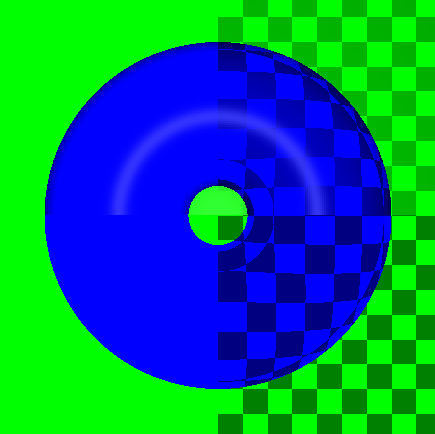
\includegraphics[width=1\linewidth]{pictures/texturundphong.png}
    \caption{Hier sieht man einen Torus mit/ohne Textur/Beleuchtung.}

    \label{fig:texturundphong}
\end{figure}

\begin{figure}
    \centering
    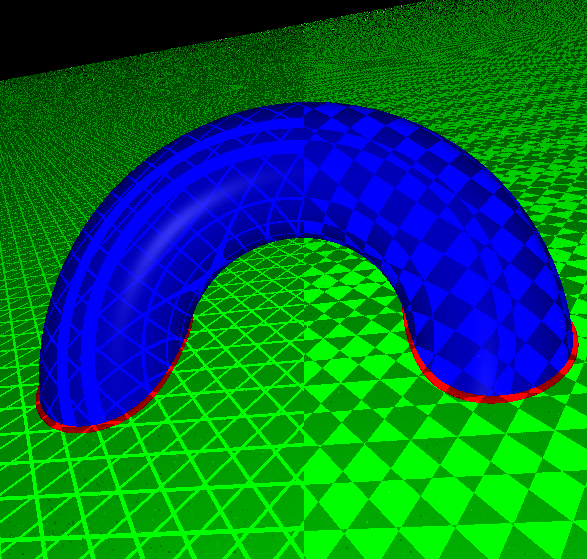
\includegraphics[width=1\linewidth]{pictures/checkerandiso.png}
    \caption{Hier sieht man die \enquote{Iso}-Textur (links) und \enquote{Schachbrett}-Textur (rechts).}

    \label{fig:checkerandiso}
\end{figure}







\chapter{Volumenbasierte Verfahren}
Die Nicht auf Raycasting basierenden Methoden konzentrieren sich darauf, grafische Primitive (Punkte, Dreiecke und Linien) zu generieren und diese dann zu visualisieren. Anders als bei \textsc{Gaalop} passiert die Auswertung des Nullraums dabei auf der GPU. Dabei ist das Anzeigen von Primitiven oft Schneller als die Raycasting Methoden. 

\section{RayMethod}
Dieses Verfahren ist prinzipiell eine Erweiterung der Ray Method aus \textsc{Gaalop}. Der Unterschied ist hauptsächlich, dass statt eines Intervallhalbierungsverfahren und Intervallarethmetik das Aberth-Verfahren zur Nullstellensuche benutzt wird.

Das Verfahren besteht aus zwei Shadern: einem Shader, der die Punktwolke generiert, und einem weiteren, der sie anzeigt.

Der Punktwolken-Erzeuger generiert achsenparallele Strahlen und verwendet das Aberth-Verfahren, um die Nullstellen entlang dieser Strahlen zu finden.

Die komplexen Nullstellen werden anschließend auf der CPU gefiltert, wieder in Punkte umgewandelt und in einen Buffer geschrieben. Da die so generierten Punktwolken Löcher haben können, wird dieser Vorgang für alle 3 Achsen ausgeführt. 


Der Vorteil dieser Methode liegt darin, dass das Rendern relativ schnell ist.


\section{Voxel-Subdivision}
\label{sec:Voxel-Subdivision}
Wenn der Raum dicht abgetastet wird, muss $f$ sehr oft evaluiert werden. Die Anzahl der Auswertungen wächst dabei kubisch mit der Größe des Gitters.
Bei einer Auflösung von 100 müsste man schon $10^6$ Punkte evaluieren. Außerdem verlieren Objekte, deren Größe nahe der Auflösung ist, alle Details.

Anstatt den ganzen Raum abzutasten, ist es deshalb sinnvoll, den Raum nur grob abzutasten und nur in der Nähe des zu visualisierenden Objektes feiner abzutasten. Dazu wird der Raum in Voxel unterteilt. Für jeden Voxel wird entschieden, ob sich Teile des Objektes im Voxel befinden, und alle Voxel, die leer sind, werden entfernt.
Dann werden die verbleibenden Voxel jeweils in 8 kleinere Voxel aufgeteilt und der Vorgang wird wiederholt, bis die Auflösung hoch genug ist.

Das Problem ist also für einen Voxel festzustellen, ob dieser leer ist. Dabei wird der Voxel durch 3 Intervalle dargestellt.
\[
\text{Voxel ist leer} \iff 0 \notin \{ f(x,y,z) | 
x \in [x_{\text{low}}, x_{\text{high}}], 
y \in [y_{\text{low}}, y_{\text{high}}], 
z \in [z_{\text{low}}, z_{\text{high}}]
\}
\]

Zur Darstellung der Voxel habe ich einfache Punktwolken genutzt, die den Mittelpunkt Visualisieren.

\subsection{Intervallarithmetik}
Eine Möglichkeit um festzustellen, ob ein Voxel leer ist, ist Intervallarithmetik. 

Um zu bestimmen, ob Teile von $f$ in einem Voxel liegen, wird der Voxel mittels Intervallarithmetik ausgewertet und geprüft, ob $0$ in dem Ergebnis liegt.
\[
0 \notin f([x_{\text{low}},x_{\text{high}}],[y_{\text{low}},y_{\text{high}}],[z_{\text{low}},z_{\text{high}}]) \implies \text{Voxel leer} 
\]

Diese Methode kann Mathematisch garantieren, dass ein Voxel leer ist. Wenn 0 im Ergebnis liegt, bedeutet dies jedoch nicht das Teile des Objektes im Voxel liegen.
Durch die Voxel-Subdivision werden die Intervalle in der nächsten Iteration kleiner. Das bedeutet das auch die Ergebnisse besser werden und mehr Voxel können entfernt werden.
Leider können die Bounds sehr groß sein was zu vielen unnötig berechneten Voxeln führt.
Das Verfahren unterteilt die Voxel bis eine maximale Unterteilungstiefe oder eine maximale Anzahl von Voxeln erreicht ist.


In der GUI heißt das Verfahren \enquote{VoxelSubdivision}.

\begin{figure}
    \centering
    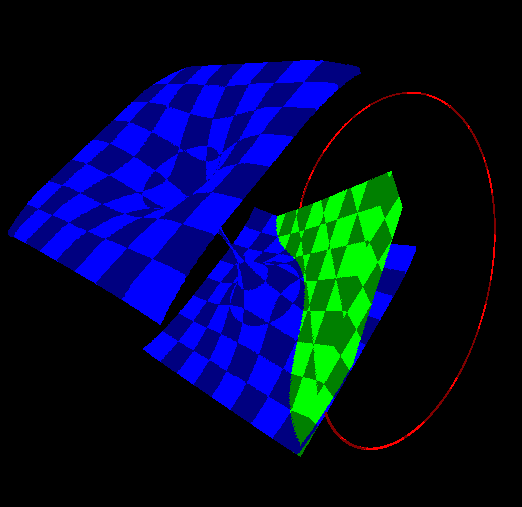
\includegraphics[width=1\linewidth]{pictures/voxeldist2.png}
    \caption{Visualisierung von Objekten mittels VoxelSubdivision. Hier sieht man einen Torusausschnitt (Blau), ein Ebenenausschnitt (Grün) und den Schnitt von Ebene und Torus (Rot).
    Dabei sieht man, dass der Ebenenauschnitt wegen der großen Bounds sehr dick ist, obwohl dieser in Theorie eine Ebene sein müsste. Außerdem kann man sehen, dass die Punkte sehr klein sind.}

    \label{fig:voxeldist2}
\end{figure}


\subsubsection{Bessere Bounds}
Um die Bounds der Intervallarithmetik zu verbessern kann \(f\) symbolisch umgeformt werden. 
Beim Testen habe ich festgestellt das die Bounds um 0 herum kleiner sind. Deshalb habe ich ein Verfahren entwickelt, dass die Funktion \enquote{verschiebt}, um sie dann um 0 herum auszuwerten. Aktuell habe ich diese Methode aus Komplexitätsgründen jedoch nicht für die aktuelle Codegenerierung reimplementiert. Deshalb ist dieses Verfahren nicht in der GUI.




Gesucht ist \(f(x,y,z)\) mit:
\[
x \in [x_0 - \delta_x,\, x_0 + \delta_x], \quad
y \in [y_0 - \delta_y,\, y_0 + \delta_y], \quad
z \in [z_0 - \delta_z,\, z_0 + \delta_z]
\]


Der erste Schritt ist das Umschreiben von \(x,y,z\):
\[
x = x_0 + I_x \cdot \delta_x, \quad
y = y_0 + I_y \cdot \delta_y, \quad
z = z_0 + I_z \cdot \delta_z
\]
\( I_x, I_y, I_z \in [-1, 1] \) sind symbolische Variablen, die die Unsicherheit repräsentieren und \( x_0,y_0,z_0 \) sind Skalare.
Dabei wird mit den Variablen \( I_x, I_y, I_z\) gearbeitet, da diese mit normalen Regeln vereinfacht werden können.
Beispielsweise ist \([-1,1]-[-1,1]=[-2,2]\) aber \(I_x-I_x=0\).



Die umgeschriebenen \(x,y,z\) Ausdrücke werden dann in die Funktion eingesetzt und die Funktion wird ausmultipliziert:

\[
f(x_0 + I_x \delta_x,\, y_0 + I_y \delta_y,\, z_0 + I_z \delta_z) = \sum_{a,b,c} c_{a,b,c} \cdot (I_x)^a (I_y)^b (I_z)^c
\]

Die Koeffizienten \( c_{a,b,c} \) hängen von den ursprünglichen Koeffizienten des Polynoms sowie von \( x_0, y_0, z_0 \) und den Skalierungen \( \delta_x, \delta_y, \delta_z \) ab. Dabei ist \(c_{0,0,0}=f(x_0,y_0,z_0)\).
Zur Auswertung wird einfach  \( I_x=[-1,1], I_y=[-1,1], I_z=[-1,1]\) eingesetzt und die Funktion kann mit den normalen Intervallarithmetikregeln ausgewertet werden.
Da diese Transformation nur aus Einsetzen und Vereinfachen besteht, bleibt die mathematische Bedeutung der Funktion exakt erhalten. Allerdings sind die Bounds des Ergebnisses oft besser. 
Im Prinzip wird eine Tailorapproximation berechnet, welche dann mittels Intervallarethmetik ausgewerted wird.
Der Nachteil der Methode ist, dass das Ausmultiplizieren relativ langsam ist.
% die bounds sind meiner meinung deshalb besser, da subtraktionen simbolisch gecancelt werden können. x*x-x*x mit x=x0+[-1,1]->[-4*x,4*x] if  not in x, aber mit ausmultiplizieren haben wir nur c_{a,b,c}=0

\subsubsection{Bound compare}
\begin{figure}
    \centering
    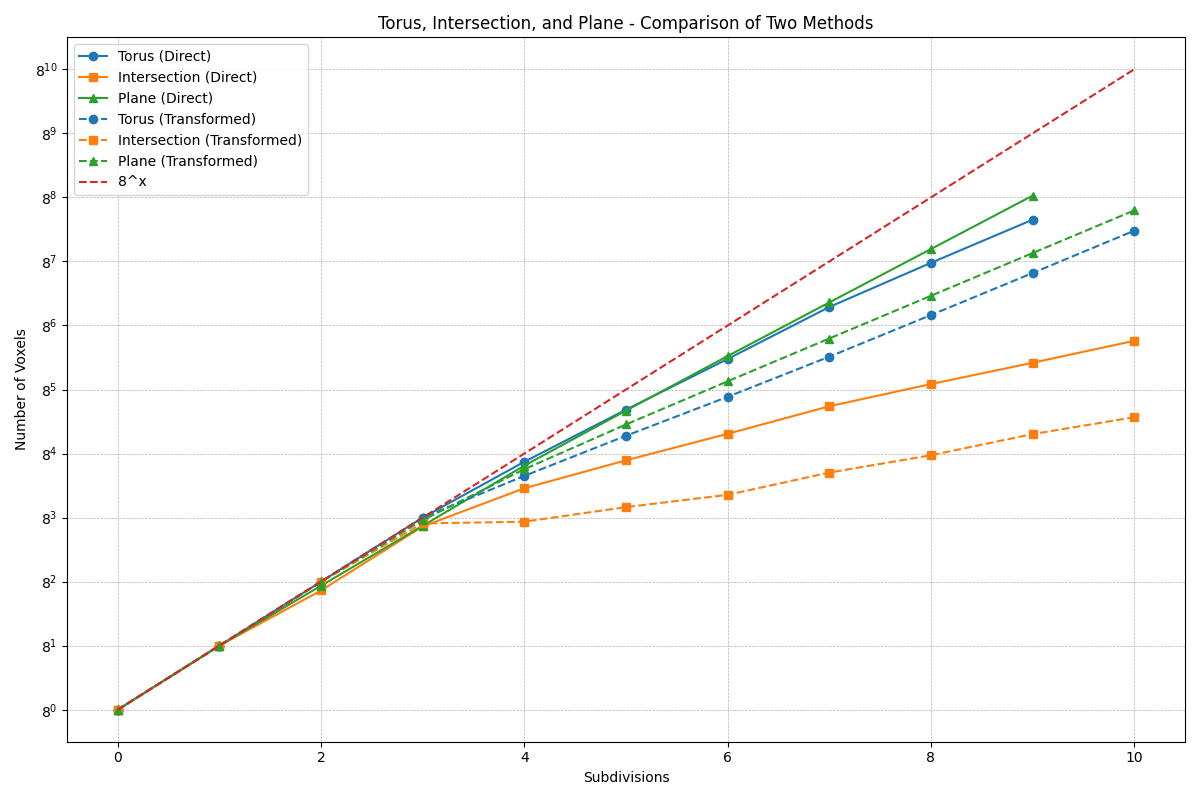
\includegraphics[width=1.0\linewidth]{pictures/FigureVoxelIntervallCompare.png}
    \caption{Die beiden Intervallarithmetik Methoden im Vergleich miteinander. Man sieht hier, dass die transformierte Intervallarithmetik etwa achtmal weniger Voxel hat (also wesentlich bessere Bounds). Die rote Linie dient als Vergleich, wenn keine Voxel entfernt würden. %Wie man sieht wird nach 10 subdivisions ca \(0.001\%\) des Raums durch die Voxel für Intersection Transformed abgedeckt. %(generiert mit intercompareplot.py)
    }
    \label{fig:enter-label}
\end{figure}


\subsection{Gauss-Newton Voxel}
Eine weitere Möglichkeit zu testen, ob ein Voxel leer ist, ist durch eine UDF. Diese wird einfach in der Mitte des Voxels ausgewertet. Dann gilt:
\[
\text{UDF}(\text{Mittelpunkt}) > \frac{\sqrt{3}}{2} \cdot \text{Kantenlänge} \implies \text{Voxel leer} 
\]

Wie schon gesagt haben wir keine UDF für \(f\). Deshalb wird wieder eine Approximation genutzt.
Eine einfache Möglichkeit für eine Approximation sind multivariate Verfahren für iterative Nullstellensuche wie das Gauss-Newton-Verfahren oder Levenberg-Marquad.
Als Startpunkt wird der Voxelmittelpunkt gewählt.
Dann werden ein oder mehrere Iterationen des Verfahrens berechnet und zum Schluss wird der Abstand zum Startpunkt berechnet.
Anders als bei der Intervallarithmetik bietet die Approximation keine mathematische Garantie und kann zu falschem entfernen von Voxeln führen.
Um dem entgegenzuwirken, kann ein Sicherheisfaktor eingeführt werden:
\[
\text{UDFApprox}(\text{Mittelpunkt}) > \frac{\sqrt{3}}{2} \cdot \text{Kantenlänge} \cdot \text{Sicherheisfaktor} \implies \text{Voxel leer} 
\]

Dabei muss beachtet werden, dass die meisten Verfahren nur lokal konvergieren. Deshalb funktioniert diese Methode am besten, um das Ergebnis der Intervallarithmetik Voxel zu filtern. Dieses Verfahren ist aktuell nicht implementiert.
\label{sec:udfvoxel} 
Ich habe stattdessen eine vereinfachte Version des Verfahrens implementiert. Dieses ist ohne Subdivision implementiert, und macht nur eine Iteration. In der GUI heißt das Verfahren \enquote{GridVoxel}. 



\section{Modifyed Marching Cubes}


Meine erste Idee zur Visualisierung von geometrischer Algebra war Marching Cubes zu benutzen. 
Marching Cubes ist ein häufig genutzter Algorithmus zur Mesh Erzeugung von Isoflächen der den Vorzeichen Übergang von Funktionen ausnutzt. Leider gibt es in \(f\) keinen Vorzeichen Übergang, da \(f\) immer positiv ist. 

Deswegen habe ich eine modifizierte Variante des Algorithmus ausgedacht.

Der normale Marching Cubes Algorithmus wertet die Funktion \( f(\mathbf{x}) \) wie die DiscreteCubeMethod auf einem äquidistanten 3D Gitter aus. Dann wird das Gitter in Würfel zerteilt, sodass die Funktionsauswertungen auf den Eckpunkten der Würfel liegen.

%mobile
Für die Meshgenerierung wird jeder Würfel einzeln betrachtet.

Auf jeder Würfelkante, die zwischen einem positiv negativ Übergang liegt, wird ein Vertex generiert. Dann wird anhand der Eckenkonfiguration (also je nachdem welche ecken positiv oder negativ sind) mittels eines lookup tables entschieden zwischen welchen Vertices Dreiecke erzeugt werden müssen. 

In meiner modifizierten Variante werden die Eckpunkte mit Ableitung betrachtet. 

Die erste Ecke wird als positive Ecke gelabelt. Dann wird zu einer benachbarten Ecke übergegangen. Falls das Skalarprodukt der Ableitungen negativ ist, wird die Ecke als negativ gelabelt und sonst als positiv. So wird auf einem Pfad durch alle Ecken gegangen bis man wieder beim Startpunkt ist. Diese angenommenen positiv/negativ Label können dann genutzt werden, um wie bei der normalen Variante das Mesh zu generieren.

Eine besondere Betrachtung ist für die Ecken mit 0 als Ableitung erforderlich. Für diese wird einfach die Ableitung der vorherigen Ecke kopiert.

Dabei baut die Marching Cubes Variante auf den Intervallarithmetik-Voxeln auf. Das bedeutet, die Voxel werden erst unterteilt und gefiltert und dann wird auf den restlichen Voxeln das Verfahren berechnet. 

Im Fall in dem \(\mathbf{F}\) nur einen Output hat, muss das Ergebnis nicht quadriert werden. In diesem Fall wird, falls es einen Vorzeichenwechsel gibt das normale Marching Cubes Verfahren benutzt.
In der GUI heißt das Verfahren \enquote{Marching Cubes}.
\section{Iterative Verfahren}
Ich habe mich entschieden die GradientMethod aus \textsc{Gaalop} nachzuimplementieren. Zusätzlich habe ich noch drei weitere iterative Verfahren hinzugefügt.
Die Verfahren starten alle auf einem voll besetzten äquidistanten 3D-Gitter an Punkten. Dann werden mehrere Iterationen berechnet, und zum Schluss werden die Punkte über einen Schwellwert gefiltert und dann als Punkte visualisiert.
Die zusätzlichen Iterationsvorschriften sind:
Newton-like:
\[\mathbf{x}^{\text{neu}} = \mathbf{x} - \frac{f(\mathbf{x})}{\|\nabla f(\mathbf{x})\|^2} \nabla f(\mathbf{x})\]
Dies ist ein Newton Schritt in Richtung des größten Gradienten.

Da dieses Verfahren teilweise nur sehr langsam konvergiert habe ich eine variante mit adaptiver schrittweite entwickelt.
GradNewton:
\[\mathbf{x}_{k+1} = \mathbf{x}_k - \alpha_k \frac{f(\mathbf{x}_k)}{\|\nabla f(\mathbf{x}_k)\|^2} \nabla f(\mathbf{x}_k)\]
Dies ist ein hybrid aus Newton-like und GradientMethod. Die Schrittweite \(\alpha\) wird immer verringert, wenn das Skalarprodukt der Ableitung und der vorherigen Ableitung kleiner null ist, und sonst erhöht.
Außerdem habe ich noch ein auf dem Levenberg Marquad Schritt basierendes Verfahren implementiert.
In der GUI heißt das Verfahren \enquote{IiterGrid}.
\section{Gitter basierte Verfahren}
TopGrid ist im Prinzip eine Reimplementierung der Discrete Cube Method aus \textsc{Gaalop}. Dabei wird nicht wie in \textsc{Gaalop} der Schwellwert für \(f\) eingestellt. Stattdessen werden die Punkte anhand der Größe des Nullraums an der jeweiligen Position sortiert, und es werden die Punkte mit den kleinsten Werten entsprechend eines einstellbaren Perzentils dargestellt.
Dabei habe ich zusätzlich zur Auswertung des Nullraums weitere Bewertungsfunktionen implementiert. Zum einen die UDF-Approximation und zum anderen die Länge eines Gauss Newton Schtrittes an dem entsprechenden Punkt.
In der GUI heißen die Verfahren \enquote{TopGrid} und \enquote{TopGridVoxel}. 
Dabei nutzt das Voxel Verfahren eine einfache auf Geschwindigkeit optimierte Version von Dual Contouring, um das Gitter als Voxel statt als Punktwolke darzustellen. 



\chapter{Implementierung}
%mobile
In diesem Kapitel geht es um die Implementierungsdetails.
Das Kapitel beginnt mit einem Überblick über die Systemarchitektur. Dann folgt im Unterkapitel Matrixvariante eine wichtige mathematische Optimierung zum Beschleunigen. Als Nächstes folgt das Unterkapitel Codegenerierung, in dem beschrieben wird, wie man vom \textsc{Gaalop} Output zur Evaluierung von \(f\) auf der GPU kommt. Dann erfolgen ein paar Performance Tests, die ich zur Analyse und zum Treffen von Designentscheidungen geschrieben habe.
Zum Schluss folgen noch ein paar einfachere Optimierungen.
\section{Systemarchitektur}
%mobile
In einem Programmdurchlauf wird immer als Erstes das von \textsc{Gaalop} generierte JSON eingelesen und als Graph deserialisiert. Dieser Graph enthält Definitionen der Nullräume der zu visualisierenden Objekte. Der Code dafür ist in der Klasse GaalopGraph.
Anschließend werden in main2.js für jedes zu visualisierende Objekt sogenannte Pipelines erstellt und gruppiert nach Objekt im RenderContext gespeichert. Dabei implementiert jede Pipeline eine Visualisierungsmethode. Die Pipelines besitzen jeweils ein oder mehrere Shader. Dabei haben die Raycasting Methoden jeweils einen Shader während die Volumenbasierten Methoden teilweise mehrere Shader zur Generierung und zum Anzeigen der Primitive haben.  
Der Shadercode wird mittels Shaderimporter eingelesen. Dieser erweitert GLSL und fügt Imports hinzu. Die meisten aktuell genutzten Shader sind im Ordner shaderlibv3.
Alle Shader welche den Nullraum auswerten sind nur Templates. Deshalb wird mittels der Codegenerierung Shadercode zur Auswertung des Nullraums aus dem eingelesenen Graph erzeugt und in den Shader eingefügt. Dies passiert in den Methoden gencode und gencodeR (Mateixvariante). Die gesamte Codegenerierung ist in der Datei codegenBackpropergation2.js zu finden.

Als Nächstes wird die Gameloop gestartet.
In jedem Gameloop-Durchlauf wird zuerst die Methode updateParams des RenderContextes aufgerufen. Diese Methode ruft die Update-Methoden der aktiven Pipelines auf. Immer wenn sich Parameter ändern, müssen die Primitive für die Volumenbasierten Pipelines neu generiert werden und auch für die Raycasting Methoden müssen teile des Graphs neu ausgewertet werden und die Shader uniforms entsprechend aktualisiert werden. 

Dann kommt die Methode \enquote{render} welche die entsprechenden render Methoden der Pipelines aufruft. Es wird nur neu gerendert, wenn sich die Parameter oder die Kamera geändert haben.
Beim Rendern wird erst ein Bild mit niedriger Auflösung gerendert und dann über mehrere Frames ein hochauflösendes Bild. Dies wird im Abschnitt \ref{sec:tilebased} näher beschrieben.
Nachdem das Bild vollständig gerendert ist, wird das Diagramm aktualisiert.

\section{Matrixvariante}


\subsection{IPNS/OPNS als Matrix Vektor Darstellung}
Die Auswertung eines Nullraums mit vielen Blades kann sehr aufwendig werden. Allerdings lässt sich der Nullraum in diesen Fällen als ein überdeterminiertes Gleichungssystem formulieren. Dadurch lässt sich der Berechnungsaufwand stark reduzieren. Dies ist essenziell für die Auswertung bestimmter Nullräume, da meine Codegenerierung sonst zu großen Shader Code erzeugt, der nicht kompilierbar ist.  

Die Multiplikation eines Multivektors mit einem anderen festen Multivektor ist eine lineare Abbildung.
Für den IPNS/OPNS wird also eine durch den zu visualisierenden Multivektor definierte lineare Abbildung auf \(\texttt{point}(x,y,z)\) berechnet.
Diese lineare Abbildung lässt sich als eine Matrix Darstellen.
Die Komponenten von \(\texttt{point}(x,y,z)\) sind Polynome über \(x, y, z\).
Zusammen lässt sich der Nullraum also als ein Gleichungssystem darstellen.
\[
M \cdot \mathbf{P}(x,y,z) = 0
\]  

Dabei kann \(M\) direkt aus dem zu visualisierenden Multivektor berechnet werden, während \( \mathbf{P}\) die Polynome aus \(\texttt{point}(x,y,z)\) darstellt. 


%!P ist glaube ich technisch gesehen keine basis

Ein konkretes Beispiel für \(\texttt{point}(x,y,z)\) in der DCGA ist:
\[
\texttt{point}(x,y,z) = x^2 e_{16} + xy\, e_{17} + xz\, e_{18} + x\, e_{19} + \tfrac{1}{2}(x^2 + y^2 + z^2)\, x\, e_{41} + \cdots + \tfrac{1}{4}(x^2 + y^2 + z^2)^2 e_{45}
\]

$\texttt{point}(x,y,z)$ könnte direkt als Vektor \(\mathbf{P}\) geschrieben werden.


In dem output von \textsc{Gaalop} liegt das Produkt $M \cdot  \mathbf{P}(x,y,z)$ nicht explizit als Matrix-Vektor-Produkt vor, sondern wird als Computational Graph umgesetzt. Es ist theoretisch möglich, $M$ und 
$\texttt{point}$ aus dem Graphen zu extrahieren, allerdings ist dies relativ aufwendig, da $\texttt{point}$ von \textsc{Gaalop} nicht vollständig synthetisiert wird.

Deswegen extrahiere ich als \(\mathbf{P}\) ein maximales linear unabhängiges Subset der Polynome aus dem Graphen die nur von \(x,y,z\) abhängen. Dies funktioniert sehr gut, allerdings ist es eine relative komplexe Lösung. Der Vorteil von diesem Ansatz ist, dass die Größe des Gleichungssystems so minimiert wird.

Der Vorteil der Darstellung $M \cdot  \mathbf{P}(x,y,z) = 0$ ist, dass sie Optimierungen erlaubt, insbesondere dann, wenn das Gleichungssystem überdeterminiert ist.
\subsection{Optimierung des Gleichungssystems}

%Vormulierung passt nicht
\( f \) kann geschrieben werden als:

\[
f = \|F\|^2 = \|M \cdot  \mathbf{P}(x, y, z)\|^2
\]

Das Interessante hierbei ist, dass die Matrix \( M \) stark verkleinert werden kann, falls sie keinen vollen Rang hat. Dadurch lässt sich auch der Auswertungsaufwand deutlich reduzieren. Gesucht ist also eine Matrix \( M' \) mit vollem Rang, für die gilt:

\[
\ker(M) = \ker(M')
\]

Mittels QR-Zerlegung lässt sich \( M \) in eine orthogonale Matrix \( Q \) und eine obere Dreiecksmatrix \( R \) zerlegen:

\[
M = Q \cdot R
\]

Falls \( M \) nicht vollen Rang hat, lässt sich \( R \) in zwei Blöcke aufteilen:

\[
R = \begin{bmatrix} R' \\ 0 \end{bmatrix}
\]

Der Ausdruck für \( f \) lautet dann:

\[
f = \|Q \cdot R \cdot P(x, y, z)\|^2
\]

Da \( Q \) orthogonal ist, bleibt die Norm unverändert, wenn \( Q \) entfernt wird:

\[
f = \|R \cdot P(x, y, z)\|^2
\]

Setzt man nun die Blockstruktur von \( R \) ein, ergibt sich:

\[
f = \left\|\begin{bmatrix} R' \\ 0 \end{bmatrix} \cdot  \mathbf{P}(x, y, z)\right\|^2 = \|R' \cdot  \mathbf{P}(x, y, z)\|^2
\]

Das bedeutet, es kann \( M' = R' \) gewählt werden.

Beachtet werden muss hierbei, dass wegen numerischer Effekte der Gleitkommaarithmetik die Zeilen von \( R \), die 0 sein sollten, nur fast null sind (im Bereich von  \( 10^{-14} \)). Allerdings funktioniert das Ganze trotzdem, wenn auch die Zeilen welche fast 0 sind, entfernt werden, um \( R' \) zu erhalten.

Eine einfache Alternative, die allerdings schwächer ist, ist durch die Ausnutzung von 
\(\ker(A) = \ker(A^TA)\).
Wenn \(M\) mehr Zeilen als Spalten hat, kann also \(f' = \|M' \cdot  \mathbf{P}(x, y, z)\|^2\) gewählt werden mit \(M' = M^\top M\). 
Dabei gilt \(f'(x,y,z)=0 \iff f(x,y,z)=0\). Weiterhin kann auch \(f =  \mathbf{P}(x, y, z)^\top M'  \mathbf{P}(x, y, z)\) berechnet werden.
Ich habe diese Alternative allerdings nicht getestet oder weiterverfolgt.


Durch beide Methoden wird die Anzahl der Zeilen der Matrix auf die Anzahl der Spalten limitiert.

\subsection{Schnelle Nullstellensuche}
\label{sec:Schnelle_Nullstellensuche}

Sei nun \(\mathbf{F}_R=R \cdot  \mathbf{P}(x,y,z)\).

Um die Nullstellensuche entlang eines Strahls zu beschleunigen, kann sie erst auf nur einer Zeile von \(R\) beschränkt werden, anstatt das ganze Gleichungssystem zu betrachten. Die reellen Nullstellen von \(f\) sind der Schnitt der Nullstellen der Komponentenpolynome von 
\(\mathbf{F}_R\). Es gilt \(f = 0 \iff \forall i\, (\mathbf{F}_R)_i = 0\). Bestimmt man also zunächst die Nullstellen einer einzelnen Komponente \((\mathbf{F}_R)_i\)(mit \((\mathbf{F}_R)_i \not\equiv 0\)), so kann man anschließend prüfen, ob dies auch Nullstellen von \(f\) sind. Die Nullstellensuche von \((\mathbf{F}_R)_i\) ist dabei wesentlich einfacher, da \((\mathbf{F}_R)_i\) einen kleineren Grad hat und schneller auszuwerten ist. Außerdem sind Nullstellen nicht unbedingt konjugate pairs was zu einer besseren Konvergenz des Aberth-Verfahrens führt.

Die Prüfung, ob die Nullstellen von \((\mathbf{F}_R)_i\) auch Nullstellen von \(\mathbf{F}_R\) sind ist allerdings komplizierter. Ich habe mich entschieden an den potenziellen Nullstellen einen Levenberg Marquad Schritt auszuwerten, um dann zu prüfen, ob die Länge dieses Schritts unter einem Schwellwert liegt. Alternativ habe ich auch eine Version implementiert, welche die UDFApprox an den Nullstellen auswerte und teste, ob diese unter einem Schwellwert liegt (Siehe \ref{sec:Nullstellentest}). 
In der GUI heißen die Verfahren \enquote{AberthGN} (Levenberg Marquad) und \enquote{Aberth} (Udf Approximation).

Weiterhin kann \(R\) und \( \mathbf{P}\) so konstruiert werden, dass \((\mathbf{F}_R)_i\) einen von i abhängen Grad hat.
Vor der Konstruktion von \(R\) können die Polynome in \( \mathbf{P}\) so sortiert werden, sodass Polynome mit niedrigerem Grad weiter unten sind. Entsprechend müssen auch die Spalten von M permutiert werden.
Das bedeutet, dass \(\deg((\mathbf{F}_R)_i)=\deg(P_i)\). Bei der Wahl von \((\mathbf{F}_R)_i\) zur Nullstellensuche kann dann das \((\mathbf{F}_R)_i\) mit dem niedrigsten Grad gewählt werden, was die Nullstellensuche theoretisch beschleunigt.
Ich habe die Sortierung implementiert, aber diesen Fakt nicht ausgenutzt, da dies die Nullstellensuche im Shader wesentlich komplexer machen würde. In der Praxis benutze ich daher immer \((\mathbf{F}_R)_1\) und lade immer das ganze \(R\) (mit Zeilen die vollkommen aus Nullen bestehen) in den Shader.




\section{Codegenerierung}
%DAG 
%topsort
%expression inlining
%graph cuttinDAG g in gpu and cpugraph

Um den von \textsc{Gaalop} generierten Rechengraph (eng computational Graph) auf der GPU auszuwerten, muss dieser zu GLSL (OpenGL Shading Language) konvertiert werden.
%i chose a dag because of memory leaks

Dies passiert in mehreren Schritten.
Als Erstes wird der Graph in \textsc{Gaalop} erzeugt und durch ein Plugin als JSON exportiert.
Dann wird das JSON in JavaScript eingelesen und wieder zu einem Graph deserialisiert.
Als Nächstes wird der Graph manipuliert. Dazu gehören Vereinfachung, Ableitungsberechnungen und Splitting.
Zum Schluss wird dann daraus Code in GLSL generiert, welcher die Auswertung in Shadern ermöglicht.
%JSON zu graph

%graph split
%graph 

\subsection{\textsc{Gaalop} Plugin}
Der erste Schritt der Codegenerierung ist das \textsc{Gaalop} Plugin.
Der Input für \textsc{Gaalop} ist ein Ausdruck in geometrischer Algebra.
\textsc{Gaalop} transformiert den geometrischen Ausdruck in eine äquivalente arithmetische Form, die aus Skalaren und klassischen Operationen besteht.
Intern wird der Ausdruck in der geometrischen Form als eine Liste von Assignment-Nodes repräsentiert.
Also etwa:
%TODO BETTER EXAMPLE
\begin{verbatim}
v=1+a
?S1=x1-0.5*(a*v)*einf;
\end{verbatim}
wird zu
\begin{verbatim}
v[0] = 1.0 + a # 1.0
S1[0] = x1 # 1.0
S1[4] = (-((a * v[0]) / 2.0)) # ep
S1[5] = (-((a * v[0]) / 2.0)) # em
\end{verbatim}

Dieser Graph wird von meinem Plugin als JSON serialisiert.
\subsubsection{computational DAG}

\subsection{DAG in js}
Das JSON wird dann von meinem Programm in einen Rechengraph umgewandelt.
Die Repräsentation als liste von Assignements eignet sich gut zur Codegenerierung und zur Serialisierung. Allerdings ist die Manipulation des Graphen in dieser Form schwierig, weshalb ich den Graphen direkt als ein DAG (directed acyclic graph) repräsentiere.
Jede Node im Graph steht dabei für eine Operation (wie Addition, Multiplikation, Division usw.) und kennt andere Operationen als Eltern.

\begin{figure}
    \centering
    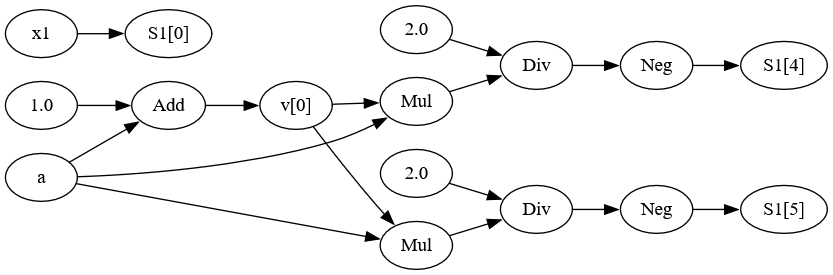
\includegraphics[width=0.5\linewidth]{pictures/daginjs.png}
    \caption{Der Beispielgraph wie er in JavaScript repräsentiert wird.}
    \label{fig:daginjs}
\end{figure}

\subsection{Graph splitting}

Um die Auswertung auf der GPU zu beschleunigen, wird der Graph in mehrere Teile geschnitten.
Auf der GPU wird der Graph zur Visualisierung später vielfach ausgewertet, wobei sich aber nur manche Variablen während der Visualisierung ändern.

Das Ganze lässt sich gut an einem Beispiel verdeutlichen. 
Im Beispiel wird die SDF einer Kugel zwischen 2 Punkten konstruiert.


\subsubsection*{Ausgangsgraph}

\begin{align*}
\text{Input: } & x, y, z, p1_x, p1_y, p1_z, p2_x, p2_y, p2_z \\
\text{Output: } & f \\[4pt]
m_x &= \frac{p1_x + p2_x}{2} \\
m_y &= \frac{p1_y + p2_y}{2} \\
m_z &= \frac{p1_z + p2_z}{2} \\
r &= \frac{\sqrt{(p1_x - p2_x)^2 + (p1_y - p2_y)^2 + (p1_z - p2_z)^2}}{2} \\
f &= \sqrt{(m_x - x)^2 + (m_y - y)^2 + (m_z - z)^2} - r
\end{align*}

Dieser Graph wird nun in Teilgraphen zerlegt.

\subsubsection*{Erster Teilgraph}

\begin{align*}
\text{Input: } & p1_x, p1_y, p1_z, p2_x, p2_y, p2_z \\
\text{Output: } & m_x, m_y, m_z, r \\[4pt]
m_x &= \frac{p1_x + p2_x}{2} \\
m_y &= \frac{p1_y + p2_y}{2} \\
m_z &= \frac{p1_z + p2_z}{2} \\
r &= \frac{\sqrt{(p1_x - p2_x)^2 + (p1_y - p2_y)^2 + (p1_z - p2_z)^2}}{2}
\end{align*}

\subsubsection*{Zweiter Teilgraph}

\begin{align*}
\text{Input: } & x, y, z, m_x, m_y, m_z, r \\
\text{Output: } & f \\[4pt]
f &= \sqrt{(m_x - x)^2 + (m_y - y)^2 + (m_z - z)^2} - r
\end{align*}

Bei der Visualisierung wird der erste Teilgraph einmal auf der CPU ausgewertet.  
Der zweite Teilgraph wird anschließend vielfach auf der GPU ausgewertet mit verschiedenen Werten für \(x,y,z\), wobei die 
Ergebnisse des ersten Teilgraphs als konstante Eingaben dienen.

Das Auseinanderschneiden des Graphen verkleinert also den GPU Graph maßgeblich (und führt zu besserer Performance).
Weiterhin macht das Auseinanderschneiden die Codegenerierung einfacher, da der Subgraph nur noch einen reduzierten Funktionsumfang hat:
Multiplikation, Division (ich glaube nur mit Konstanten), Subtraktion, Addition und Negation.
\subsection{Graph Manipulationen}
Bevor der Subgraph auf der GPU ausgewertet werden kann, muss er manipuliert werden. Das liegt daran, dass manche der Methoden Ableitungen erfordern oder Auswertung über den komplexen Zahlen.

Der Shadercode enthält Funktionsheader, welche dann durch den in JavaScript
generierten Shadercode ersetzt werden.

\subsubsection{Was generiert die Codegenerierung}
Die alte Codegenerierung generierte Code für die folgenden Methoden:

\begin{itemize}

\item
\begin{minted}{glsl}
float Summofsquares(vec3 rayDir, vec3 rayOrigin, float a)
\end{minted}
Diese Methode wertet \(f\) aus.

\item
\begin{minted}{glsl}
xyzDual xyzDualSummofsquares(vec3 pos)
\end{minted}
Diese Methode wertet \(f\) und \(\nabla f\) aus.

\item
\begin{minted}{glsl}
void DualF(vec3 rayDir, vec3 rayOrigin,
           float a, out Dual[numoutputs] result)
\end{minted}
Diese Methode wertet \(\mathbf{F}(\mathbf{ray}(a))\) und
\(\frac{dF(\mathbf{ray}(a))}{da}\) aus.

\item
\begin{minted}{glsl}
DualComplex DualComplexSummofsquares(
    vec3 rayDir, vec3 rayOrigin, Complex a)
\end{minted}
Diese Methode wertet \( f_{\text{ray}}(t) \) und
\(\frac{df(\mathbf{ray}(a))}{da}\) mit komplexen Zahlen aus.
Dies wird für die Aberth-Verfahren benötigt.

\item
\begin{minted}{glsl}
Intervall IntervallSummofsquares(
    Intervall _V_X, Intervall _V_Y, Intervall _V_Z)
\end{minted}
Diese Methode wertet \(f\) mittels Intervallarithmetik aus.

\item
\begin{minted}{glsl}
bool evaluatevoxelIntervall3d(
    Intervall x, Intervall y, Intervall z)
\end{minted}
Diese Methode wertet \(f\) mittels Intervallarithmetik aus und
gibt zurück, ob \(0\) im Ergebnisintervall enthalten ist.

\end{itemize}

Dabei muss beachtet werden, dass alle Methoden mit
\texttt{Summofsquares} im Namen im Fall eines einzelnen Outputs
nicht das Quadrat berechnen. In diesem Fall gilt \(f =  \mathbf{F}\) statt \(f = |\mathbf{F}|^2\).
Ich hatte dies anfangs implementiert um das normale Aberth-Verfahren zur schnelleren Konvergenz nutzen zu können.


Zusätzlich zu den Funktionen werden noch einige Variablen berechnet:

\begin{itemize}

\item
\begin{minted}{glsl}
uniform float[?] args;
\end{minted}
\texttt{args} sind die Argumente des GPU-Teilgraphs.

\item
\begin{minted}{glsl}
int numoutputs = ?;
\end{minted}
Die Anzahl der Outputs von \(\mathbf{F}\).

\item
\begin{minted}{glsl}
int POLYDEGREE = ?;
\end{minted}
Der Polynomgrad der \texttt{Summofsquares}-Methoden.

\item
\begin{minted}{glsl}
#define USE_DOUBLEROOT
\end{minted}
Dieses Makro zeigt an, dass \(f = \mathbf{F}\) statt \(f = |\mathbf{F}|^2\)
verwendet wurde.

\end{itemize}


Die neue Codegenerierung kann alles generieren, was die alte Codegenerierung generieren konnte. Zusätzlich wird der Code für die Matrixvariante generiert. Dabei hat die Matrixvariante ähnliche Methoden mit leicht anderen Namen die praktisch das Gleiche berechnen.

Aktuell wird nur noch die Matrixvariante benutzt.

%void MatmulRDense(vec4[basislength] P,out vec4[basislength] b){?}
%void MatmulRDense(vec2[basislength] P,out vec2[basislength] b){?}

%Matrix mul eines Vectors mit R. Diese funktionen müssen generiert werden da der code ausgerollt wird.

%void makeDualComplexP(vec3 rayDir, vec3 rayOrigin,Complex a,out DualComplex[basislength] P) {?}
%berechnet P,dPda im komplexen
%void makeP(vec3 pos,out float[basislength] P) {?}
%berechnet  P
%void makexyzDualP(vec3 pos,out xyzDual[basislength] P) {?}
%berechnet P,dPdx,dPdy,dPdz
%void makeDualP(vec3 rayDir, vec3 rayOrigin,float a,out Dual[basislength] P) {?}
%berechnet P,dPda 
%void makeIntervallP(Intervall X,Intervall Y,Intervall Z,out Intervall[basislength] P) {?}
%berechnet P über intervall arithmetik
%float susRDenseUnrolled(vec3 pos){?}
%wertet f aus

%alte ansätze
Anfangs habe ich zur Ableitungsberechnung duale Zahlen verwendet. Dies ließ sich relativ einfach implementieren, hat aber den Nachteil, dass der Graph typisiert werden muss. Anstatt nur mit Skalaren zu arbeiten, gibt es für die komplexen Zahlen, Duale komplexe Zahlen, Skalare, Duale mit mehreren Inputs und Intervalle. Weiterhin müssen auch Interaktionen zwischen verschiedenen Typen (beispielsweise die Multiplikation von einem Skalar mit einer Dual Zahl) ausprogrammiert werden, was zu einer kombinatorischen Explosion führt. Und dann muss später für jede der Kombinationen eine Methode zu Codegenerierung geschrieben werden. 

Mein erster Ansatz bestand darin für jeden Typ neue Codegenerierung zu schreiben. Dabei gab es in der Regel zwei Typen pro Codegenerierung. Skalare und den Typ, über dem die Codegenerierung stattfindet. Wenn beispielsweise über den komplexen Zahlen ausgewertet wurde, waren die gesplitteten Inputs von der CPU Skalare und die sich ändernden Variablen komplexe Zahlen. Alle Operationen zwischen Skalaren und anderen Typen haben dann den anderen Typen als Output. Also beispielsweise:
Mul(skalar a,Complex b)-> Complex

Dabei habe ich oft den Skalar einfach hochkonvertiert. Also statt Mul(Skalar a, Complex b) zu implementieren, kann Mul(Complex a, Complex b) benutzt werden, wobei a zu einer komplexen Zahl gecastet wird. Das macht das Ganze einfacher, aber auch langsamer.
Die Typen waren unter anderem: Skalare, komplexe Zahlen, duale Zahlen, komplexe Duale, Intervalle, 3D-Duale.
Dieser Ansatz war relativ unflexibel und unübersichtlich. Anfangs ging es noch, allerdings hatte ich weitere Ideen und habe dann immer mehr Typen hinzugefügt.

%explain type propergation

Mein nächster Ansatz war es, typisierte Nodes zu machen. Dabei habe ich den Code für Codegenerierung und Typ-Propagation in die Nodes gepackt, statt eigene Klassen zur Codegenerierung zu schreiben.
Typ-Propagation bedeutet dabei, dass jeder Node ein Typ zugeordnet werden muss welcher sich auch auf die Codegenerierung auswirkt. Beispielsweise muss eine MulNode die zwei Skalare als input hat anderen Code generieren als eine MulNode welche ein Dual und ein Skalar als input hat. 
Der Vorteil von diesem Ansatz war, dass er wesentlich flexibler ist und einfacher zu erweitern. Weiterhin ermöglicht dieser Ansatz die Auswertung des Ganzen auf der CPU. Der Nachteil von diesem Ansatz war, dass er wesentlich größer ist, weshalb ich irgendwann abgebrochen habe. Dies liegt daran, dass für alle Typ-Kombinationen für jeden Node-Typ (MulNode,AddNode,AbsNode usw.) Code zur Codegenerierung und Auswertung geschrieben werden musste.

Als Nächstes habe ich mich entschieden, die Ableitungsberechnung auf Backpropagation und Forward-Mode-Autodiff umzustellen. Dies hat zwei große Vorteile.
Erstens gibt es nur noch drei Typen: Skalare, komplexe Zahlen und Intervalle, was die Codegenerierung wesentlich einfacher macht. Und zweitens müsste Backpropagation theoretisch bei manchen Ansätzen schneller sein, da weniger Multiplikationen benötigt werden.

Im aktuellen Ansatz habe ich versucht, die anderen Ansätze zu vereinigen.
Ich habe mich entschieden, die Typ-Propagation während der Codegenerierung zu machen, wobei ich den Code dafür in die Nodes gepackt habe. Das macht den Code kleiner, allerdings ist das typisierte Auswerten in JavaScript nicht möglich.
Die neue Codegenerierung ist flexibler, weniger komplex und hat weniger Bugs. Da es in der alten Codegenerierung für jede Funktion eine eigene Klasse zur Codegenerierung gab, war es wesentlich schwerer, Bugs zu fixen, da sie teilweise in jeder der Klassen gefixt werden mussten. Dies war der Hauptgrund, weshalb ich die neue Codegenerierung geschrieben habe.

Ein Problem, das in beiden Codegenerierungen besteht, ist, dass der generierte Code teilweise nicht kompilierbar ist, da er zu groß ist.
Teilweise haben Multivektorprodukte Hunderte an Outputs, was bedeutet, dass der WebGL2-Compiler ohne Fehlermeldung aufgibt, wobei zusätzlich teilweise der WebGL2-Kontext abstürzt. Die Matrixvariante der neuen Codegenerierung löst dieses Problem.

\subsection{Vereinfachung}
Durch die Manipulation des Graphen entstehen Artefakte wie beispielsweise Multiplikation mit 1. Deshalb wird der Graph vereinfacht. Zu den Vereinfachungen gehören unter anderem:
Eliminierung von konstanten Subausdrücken,
Common Subexpression Elimination und
Entfernen von Addition mit 0 und Multiplikation mit 1.



\subsection{Matrix Extraktion}
Für die Matrixvariante muss die $M$ und $\mathbf{P}(x,y,z)$ aus dem Graphen extrahiert werden.

Ich habe zwei Versionen der Matrixextraktion aus dem Graph geschrieben.  

Die alte Version berechnet nur $M$ und nimmt an, dass $\mathbf{P}$ gegeben ist. Der Nachteil dabei ist, dass $\mathbf{P}$ von der Algebra abhängt, was bedeutet, dass für jede Algebra $\mathbf{P}$ vordefiniert werden müsste. Die neue Version hat dieses Problem nicht und baut $\mathbf{P}$ automatisch.  

In der alten Version wird der GPU-Teilgraph zunächst im Prinzip symbolisch ausmultipliziert. Dabei werden die Polynome als Summe von Monomen über $x, y, z$ mit zugehörigen Koeffizienten dargestellt, wobei alle übrigen Variablen in die Koeffizienten einfließen.  

Beispielsweise wird
\[
(x \cdot x + y \cdot y + z \cdot z)\cdot (a \cdot b + c) + x \cdot x \cdot d
\]
zu
\[
(ab + c + d)\cdot x^2 + (ab + c)\cdot y^2 + (ab + c)\cdot z^2.
\]

Dabei erfolgt die Darstellung als Polynom in $x, y, z$, während alle anderen Terme als skalare Koeffizienten behandelt werden.  

Das Ergebnis ist also ein Polynom für jede Komponente des Output-Multivektors.  
Um diese Polynome in der Polynombasis der Algebra zu repräsentieren, wird mittels einer Basiswechselmatrix von der Monombasis zur Polynombasis $\mathbf{P}$ der Algebra konvertiert. Somit erhält man $M$.  

Im neuen Ansatz müssen als Erstes die Polynome von $\mathbf{P}$ extrahiert werden. Dazu werden alle Nodes aus dem Graph extrahiert, die nur von den Variablen $x, y$ oder $z$ abhängen.  

%mobile  
Der nächste Schritt ist die Auswahl einer maximal linear unabhängigen Untermenge dieser Nodes, welche als eine Polynombasis verwendet werden kann. Dafür wird für jede Node ein Koeffizientenvektor in einer Monombasis und die Anzahl der Vorfahren berechnet.  
Die Nodes werden nach Anzahl der Vorfahren sortiert und dann der Reihe nach zu $\mathbf{P}$ hinzugefügt, falls sie linear unabhängig von den schon hinzugefügten Polynomen sind. Ich nutze dazu eine modifizierte Version des modifizierten Gram-Schmidtschen Orthogonalisierungsverfahrens \cite{wikipedia_gram_schmidt}.  
%https://en.wikipedia.org/wiki/Gram%E2%80%93Schmidt_process  

Nachdem $\mathbf{P}$ vollständig ist, wird im Prinzip der alte Ansatz genutzt, um $M$ zu erhalten.  

Durch das Ausmultiplizieren und die Multiplikation mit der Basiswechselmatrix kann der CPU-Teilgraph wesentlich größer werden. Deshalb ist dieser Ansatz schnell auf der GPU, aber langsam auf der CPU. 
Da die CPU jedoch wesentlich weniger Auswertungen macht, ist dies jedoch nicht wirklich ein Problem.  

Zwischendurch habe ich einfach eine Monombasis für $\mathbf{P}$ verwendet, da diese im Ausmultiplizierungsschritt entsteht. Dies funktioniert auch, ist aber langsamer und instabieler auf der GPU.

\section{Performance-Analyse}


\subsection{Alte Codegenerierung vs neue Codegenerierung}
Ich habe wie schon gesagt die neue Codegenerierung nicht aus Performancegründen geschrieben. Trotzdem habe ich eine einen kleinen Test zum Vergleich der Ausführungszeiten gemacht, um dafür zu sorgen, dass die Ausführungszeiten vergleichbar sind.
Dieser Findet sich in testcodegenbackproptestall.html.

\begin{figure}
    \centering
    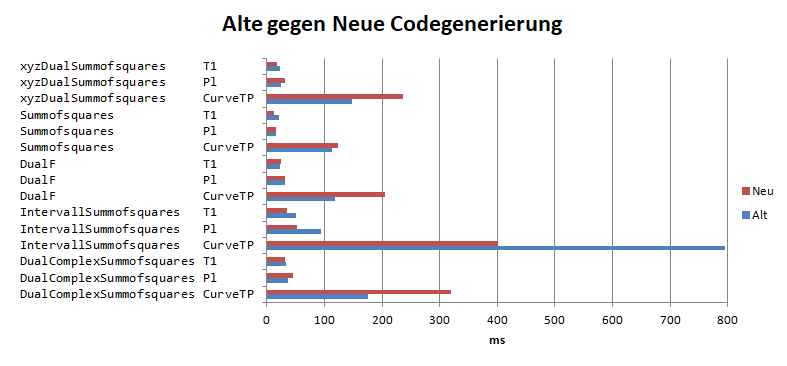
\includegraphics[width=0.5\linewidth]{pictures/CodegenAltVSNewTimings.png}
    %\caption{}
    \label{fig:CodegenAltVSNewTimings}
\end{figure}

Die Ergebnisse zeigen, dass die neue Codegenerierung manchmal schneller ist und manchmal die alte. Ich bin mir nicht sicher, warum dies so ist. Hier sind meine Theorien:

Ein Vorteil der alten Codegenerierung könnte sein, dass der Compiler durch die vielen Typen ein besseres Memory Layout erzeugen kann und weniger Operationen benötigt. Beispielsweise sieht der Code für die Multiplikation bei \texttt{xyzDual} folgendermaßen aus:

\begin{minted}{glsl}
xyzDual xyzDualMul(xyzDual a,xyzDual b){
    return xyzDual(a.w*b.xyz+b.w*a.xyz,a.w*b.w);
} 
\end{minted}

Dieser Code berechnet im Prinzip Forwardpropagation für eine Multiplikation mit drei Variablen gleichzeitig. Teilweise kann die Multiplikation mit drei Variablen (\texttt{a.w*b.xyz}) mit nur einer Instruktion passieren.
Weiterhin sind \texttt{xyzDual} im Grunde umbenannte \texttt{vec4}s, was bedeutet, dass sie oft in ein Register passen.
Der Code der neuen Codegenerierung benutzt Backpropagation/Forwardpropagation auf der Graph-Ebene und erzeugt danach den Code. Das macht es dem Compiler schwerer, die Multiplikationen zu bündeln.
Das Ganze ist natürlich stark vom Compiler und der Hardware abhängig.
Ein Vorteil des neuen Codes könnten bessere Vereinfachungen des Graphen sein.


\subsection{Schnelle Matrix-Vektor-Multiplikation in Glsl}
Um \(\mathbf{F}_R=R\cdot\mathbf{P}(x,y,z)\) für den Matrixansatz auszuwerten wird Matrixmultiplikation in GLSL benötigt, die möglichst performant sein muss. Kleine Änderungen im Shadercode machen große Performance-Unterschiede. Deshalb habe ich viele Tests gemacht um eine schnelle Version zu finden.
Um diesen Abschnitt vollständig zu verstehen ist es sinnvoll sich den Testcode anzuschauen.
Der Testcode ist in unrolled.js und kann mittels speedtestharness.html ausgeführt werden. 

Es mehrere Parameter die geändert werden können. 
Die Matrix als uniforms oder als uniform Buffer (ubo) hochgeladen werden. 
Da \(R\) eine obere Dreiecksmatrix ist, kann außerdem nur die Obere Rechte Hälfte oder die ganze Matrix hochgeladen werden. Alle mit M gekennzeichneten Tests benutzen die volle Matrix und alle mit \(R\) gekennzeichneten die Hälfte.
Weiterhin kann die Matrix normal oder dicht gepackt als vec4 hochgeladen werden. Dabei wird jede Zeile mit Nullen aufgefüllt, um eine Länge die ein Vielfaches von 4 ist zu erhalten. Die dicht gepackten Versionen werden dabei als Dense bezeichnet.
Zudem kann die Auswertung ausgerollt werden.

Diese Parameter können beliebig kombiniert werden und Ich habe viele (aber nicht alle) Kombinationen getestet.
Auch der Browser (Ich habe Firefox und Edge getestet) spielt eine große Rolle.


Ich habe hauptsächlich 4 verschiedene Methoden ausgewertet. 
\enquote{sus} steht für \enquote{sum of squares} und ist die normale Auswertung von \(f\).
Außerdem gibt es noch \enquote{row} was dafür steht das nur die erste Zeile der Matrix zur Auswertung genutzt wird (also \((\mathbf{F}_R)_1\)). Diese Methode wertet das Skalarprodukt von der ersten Zeile der Matrix mit \(\mathbf{P}\) aus.
Weiterhin wird für die Aberth-Verfahren auch die Auswertung im Komplexen mit Ableitung benötigt. Deshalb gibt es beide Methoden nochmal mit DC was für Dual Complex steht.
Dann gibt es noch horner was eine Auswertung über die mittels der Vandermonde-Matrix approximierten Koeffizienten des Polynoms ist (mehr dazu in Abschnitt \ref{sec:Auswertung_über_Koeffizienten}). Weiterhin gibt es bei row noch Methoden mit \enquote{copy} im Namen. Diese kopieren die erste Zeile der Matrix in ein Array und benutzen dann dieses Array zur Auswertung.

Getestet habe ich auf einem Laptop mit einer Geforce gt 730M was eine Grafikkarte von 2013 ist.
Alle Tests wurden in einem Vertex-Shader mit 100000 Vertices ausgeführt. Um Overhead zu vermeiden, werden im Shader zusätzlich mehrere Iterationen ausgeführt. Erst eine, dann 10, dann 100 usw. bis der Test länger als 100 ms dauert.
Das Ergebnis ist die minimale Zeit pro Iteration bei 20 Wiederholungen. 
Berechnet wird immer (außer für horner) \(\mathbf{P}\) und dann die Multiplikation mit der ersten Zeile der Matrix für \enquote{row}. Für \enquote{sus} wird die Summe der Quadrate der Multiplikation von \(\mathbf{P}\) mit der ganzen Matrix berechnet. Die Matrix ist dabei eine 25x25 Matrix was einer Monombasis vierten Grades entspricht.



\begin{figure}
    \centering
    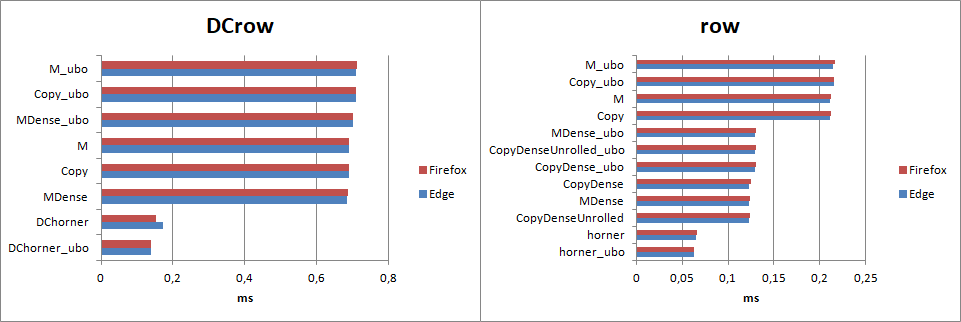
\includegraphics[width=1\linewidth]{pictures/row_times_cleaned.png}
    \caption{Performance bei der Auswertung von $(F)_1$ (rechts) und $(F)_1$ mit Ableitung im Komplexen (links) mittels verschiedener Methoden.}
    \label{fig:row_times_cleaned}
\end{figure}

Die Ergebnisse für row und DCrow (siehe \ref{fig:row_times_cleaned}) sind relativ einfach zu verstehen. Die Approximation durch Horner ist am schnellsten, da am wenigsten Multiplikationen benötigt werden. Weiterhin sind die dichten Methoden für row schneller. Das liegt daran, dass für diese dot benutzt werden kann, wodurch weniger Multiplikationen benötigt werden.

Weiterhin sind die ausgerollten Methoden genauso schnell wie die anderen, weshalb ich vermute, dass der Compiler die Schleife intern ausrollt. Eine interessante Sache hierbei sind die Copy-Methoden. Diese ermöglichen das Kopieren der nicht-dichten Arrays in dichte Arrays und somit eine schnelle Evaluation, egal wie die Matrix hochgeladen wurde.

\begin{figure}
    \centering
    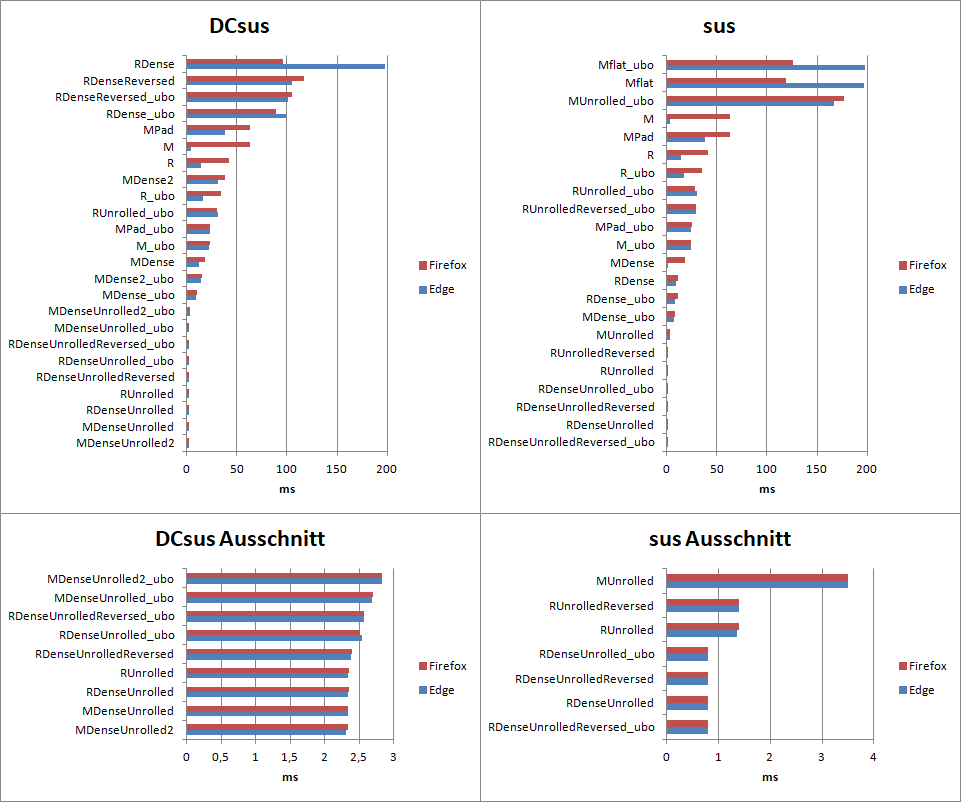
\includegraphics[width=0.5\linewidth]{pictures/sustimes_cleaned.png}
    \caption{Performance bei der Auswertung für \( f\) und \( f_{\text{ray}}(t) \) (rechts) sowie \( f_{\text{ray}}(t) \) mit Ableitung im Komplexen (links) mittels verschiedener Methoden. Das untere Diagramm ist ein vergrößerter Ausschnitt des oberen Diagramms. }
    \label{fig:sustimes_cleaned}
\end{figure}
Ich habe die Timings für \enquote{DCsus} und \enquote{sus} sind im Diagramm \ref{fig:sustimes_cleaned} sichtbar. Die ausgerollten Versionen sind wesentlich schneller als die nicht ausgerollten Versionen und für \enquote{sus} sind die Dichten Versionen wie auch bei \enquote{row} schneller. Die dichten Versionen sind komplizierter zu programmieren, weshalb es auch die \enquote{Reversed} Versionen gibt, welche die Multiplikation mit einer gespiegelten Version von \(R\) berechnen, was die Schleifenlogik einfacher macht. Ein Ausreißer für DCsus scheint Runrolled\_ubo zu sein. Ich vermute, dass liegt daran, dass \(R\) auf dem ubo 4-mal größer ist (da WebGL2 nur std140 unterstützt) und deshalb die Matrix in einen anderen Speicherbereich lädt. Allerdings bin ich mir nicht sicher. Weiterhin ist noch MDenseUnrolled2 interessant. Diese Methode macht erst die Matrix Multiplikation in einer separaten Funktion und dann die Akkumulation der Summe der Quadrate. Dies ist etwas langsamer aber der Code lässt sich besser wiederverwenden. Letztendlich habe ich mich für eine Kombination aus MDenseUnrolled2 und RDenseUnrolled entschieden. Das bedeutet ich benutze RDense und habe eine Funktion für eine Multiplikation mit einem Vektor. 
Für RDense gibt es für alle Fälle schnellen Code zur Evaluierung der Funktion. Für row muss beachtet werden, dass der Code für \(M\) und \(R\) prinzipiell gleich ist, weshalb einfach die MDense Varianten genutzt werden können.

\section{Optimizations}
\subsection{Adaptive Auflösung}
%Tile-based
Manche der Raycasting-Methoden sind relativ langsam, was zu niedrigen FPS führt. Dies macht die Oberfläche praktisch unnutzbar.
Teilweise konnten Frames über eine Sekunde dauern. Dies kann zu einem Timeout und somit zu einem Absturz des OpenGL-Kontextes führen. Der Kontext kann nach einem Absturz nicht von innerhalb der Anwendung wieder hergestellt werden, nur durch Neuladen des Tabs oder teilweise Neustarten des Browsers kann ein neuer Kontext erschaffen werden.
Deshalb hatte ich anfangs die Auflösung verringert, solange der Nutzer die Kamera bewegt, um stattdessen wesentlich mehr FPS zu generieren. Diese Optimierung ist relativ einfach zu implementieren und führt zu wesentlich angenehmerer Kamerabewegung. Auch die maximale Auflösung war reduziert, um Abstürzten des OpenGL-Kontextes zu verhindern.

\subsection{Tile-based Rendering}
\label{sec:tilebased}
Um trotzdem mit hoher Auflösung rendern zu können, habe ich dann einen Tile-based Rendering Ansatz implementiert. 
Dazu wird der Bildschirm in rechteckige Tiles (Kacheln) unterteilt, die dann nacheinander gerendert werden können. Der Vorteil dieses Ansatzes ist, dass so mit voller Auflösung gerendert werden kann, ohne den OpenGL Kontext zu crashen. Weiterhin kann das rendern zwischendrin abgebrochen und von neu begonnen werden, falls sich die Kamera bewegt oder sich Parameter ändern, was zu einer schnellen Reaktion führt. Wie auch bei dem vorherigen Ansatz wird auch bei diesem Ansatz vor dem Tile-based Rendering das Bild in niedriger Auflösung gerendert, damit der Nutzer schnell ein neues Bild erhält.

Dabei muss beachtet werden, dass Tile-based Rendering (oder das Rendern mit kleiner Auflösung) nur hilft, wenn der Vertex-Shader nur wenig Arbeit verrichten muss, da für jedes gerenderte Tile der Vertex-Shader für alle Vertices neu durchlaufen werden muss. 
Beim Rendern einer Punktwolke passiert im Vertex-Shader beispielsweise die Transformation der Punkte mit der Kameramatrix und Projektionsmatrix. Bei vielen Punkten ist das Tile-based Rendering deshalb wesentlich langsamer.
Deshalb werden die Shader, welche tilebar sind (also nur wenige Vertices und leichtgewichtiger Code im Vertex-Shader) von den anderen separat gerendert. Das Ganze funktioniert folgendermaßen:

Im ersten Frame werden die Shader, welche nicht tilebar sind, in einen Framebuffer mit voller Auflösung gerendert, während die Shader, welche tilebar sind, in einen Framebuffer mit niedriger Auflösung gerendert werden. Anschließend werden beide Buffer auf den Bildschirm gemalt, wobei der mit der niedrigen Auflösung hochskaliert wird.

In den nächsten Frames wird jeweils ein Tile pro Frame gerendert. Dafür werden die tilebaren Shader direkt in einem Ausschnitt auf den Bildschirm gerendert. Für die nicht tilebaren Shader liegt das Ergebnis für den entsprechenden Ausschnitt bereits im Framebuffer vor und kann einfach \enquote{kopiert} werden.


Anfangs hatte ich die Tiles in von links nach rechts und von oben nach unten gerendert. Später habe ich mich dazu entschieden die Tiles von der Mitte nach außen zu rendern, um die wichtigen Bildinhalte tendenziell zuerst in hoher Auflösung zu rendern.

Die Implementierung lässt sich in der Datei MultiresBuffer3.js finden.


%Todo implement tile based


\subsection{Polynom-Auswertung über Koeffizienten}
\label{sec:Auswertung_über_Koeffizienten}
In den Raycasting-Methoden wird \( f_{\text{ray}}(t) \) sehr häufig ausgewertet. Da \( f_{\text{ray}}(t) \) ein Polynom ist, kann man die Koeffizienten für dieses Polynom berechnen und dann in Zukunft die Funktion anhand dieser Koeffizienten auswerten. Die Auswertung anhand der Koeffizienten kann wesentlich schneller sein, da in der Regel wesentlich weniger Multiplikationen benötigt werden.

Die Koeffizienten berechne ich dabei mittels einer Vandermonde-Matrix (Siehe \ref{sec:Vandermonde}).  
%TODO count multiplications and compare

Leider scheint diese Optimierung numerisch sehr instabil zu sein, was zu einem sehr verrauschten Bild führt. In der Nähe der Kamera ist das Rauschen kleiner, aber immer noch relativ groß. Ich vermutete, dass das daran liegt, dass ich Stützstellen nahe der Kamera gewählt habe.

Eine andere Möglichkeit für das Berechnen der Koeffizienten ist das Ausmultiplizieren. Diese Methode ist wesentlich aufwendiger zu implementieren und hat leider auch nicht zu wesentlich besseren Ergebnissen geführt.  Wahrscheinlich könnte eine bessere Wahl für eine Polynombasis zu wesentlich besseren Ergebnissen führen.


Eine Möglichkeit die Ergebnisse zu verbessern ist durch eine Reskalierung des Polynoms \cite{flocke2015algorithm954}. 
Sei 
\[
k = \frac{1}{\max\left\{ |\frac{a_{n-1}}{a_n}|,\; |\frac{a_{n-2}}{a_n}|^{1/2},\; \dots,\; |\frac{a_{1}}{a_n}|^{1/(n-1)},\; |\frac{a_{0}}{a_n}|^{1/n} \right\}}
\]
dann sind die Nullstellen von \(f_\text{approx}(\frac{x}{k})\) im Intervall \([-2,2]\). Allerdings ist diese Version nur ein bisschen stabiler, weshalb ich sie nicht benutzt habe (siehe \ref{fig:aberth_rescaled}). 


Ich habe anfangs auch mit Lösungen in geschlossener form experimentiert, allerdings funktionieren diese nur für Polynome bis zum 4ten-Grad und weiterhin haben sie das gleiche Problem wie das auf Koeffizienten basierte Aberth-Verfahren. Die Ergebnisse sind verrauscht.
Darüber hinaus habe ich den in \cite{peters2023gpuPolynomialRoots} beschriebenen Ansatz zur Nulstellensuche untersucht. Allerdings hat auch dies nicht weitergeholfen.

Eine Möglichkeit, die verrauschten Ergebnisse nutzbar zu machen, ist, erst eine verrauschte Näherung für die Nullstellen mit \(f_\text{approx}\) zu berechnen, um dann \(f\) normal auszuwerten, um mit den angenäherten Nullstellen weiter zu rechnen. Dadurch bleibt die Qualität erhalten und es kann ein kleiner Performance-Boost für das Aberth-Verfahren beobachtet werden. 
Dabei passt dieses Verfahren besonders gut zu der im Abschnitt~\ref{sec:Schnelle_Nullstellensuche} beschriebenen Methode da diese mit Polynomen kleineren Gerades arbeitet. Dies macht die Vandermonde-Matrix kleiner und das Verfahren stabiler.



\begin{figure}
    \centering
    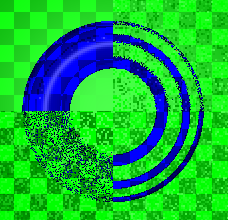
\includegraphics[width=0.5\linewidth]{pictures/aberth_rescaled_test.png}
    \caption{Oben links: $f$, oben rechts: $f_{\mathrm{approx}}\!\left(\frac{x}{k}-1\right)$, unten links: $f_{\mathrm{approx}}(x)$, unten rechts: $f_{\mathrm{approx}}\!\left(\frac{x}{k}\right)$ }
    \label{fig:aberth_rescaled}
\end{figure}


\chapter{Evaluierung}
\IMRADlabel{results}



\section{Volumenbasierte Verfahren}
\textsc{Gaalop} hat einen integrierten Visualisierer. Allerdings hat \textsc{Gaalop}s Visualisierer kein Graph Splitting und evaluiert immer den ganzen Graph. Deshalb kann der Visualisierer sehr langsam sein, wenn der Graph groß ist. Große Graphen entstehen vor allem durch Variablen im Graph. Das folgende Beispiel erzeugt einen Torus, eine Ebene, und deren Schnitt in DCGA.
\begin{verbatim}
//algebra DCGA
T1 = Toroid(R1, r1);                
Pl = Plane(nx, ny, nz, d);    
CurveTP = T1 ^ Pl;     
:Blue;
:T1;

:Red;
:CurveTP;

:Green;
:Pl;     
\end{verbatim}
Im Visualisierer von \textsc{Gaalop} kann man jetzt die Variablen einstellen und dann den Ausdruck visualisieren lassen.
Alternativ kann man die Variablen auch direkt in den Code schreiben:
\begin{verbatim}
//algebra DCGA
T1 = Toroid(1, 1);                
Pl = Plane(1, 1, 1, 0);    
CurveTP = T1 ^ Pl;     
:Blue;
:T1;

:Red;
:CurveTP;

:Green;
:Pl;     
\end{verbatim}
Der Nachteil dabei ist, dass man die Variablen natürlich nicht mehr einstellen kann. Allerdings ist das Visualisieren so viel schneller, da der erzeugte Graph viel kleiner ist. Das liegt daran, dass konstante Subgraphen zur Kompilezeit ausgewerted werden können. Deshalb habe ich jeweils zwei Performancemessungen in \textsc{Gaalop} gemacht. In meinem Visualisierer ist die statische Szene auch etwas schneller, allerdings ist der Unterschied kleiner, weshalb ich meine Zeitmessungen nur mit der dynamischen Szene gemacht habe.

Im Folgenden werde ich diese Szene in \textsc{Gaalop} und meiner Visualisierung vergleichen.

\subsection{Iterative Verfahren}
Wie schon gesagt habe ich die GradientMethod aus \textsc{Gaalop} nachimplementiert.
\textsc{Gaalop}s Default-Parameter sind maximal 50 Iterationen bei einer Gitter-Kantenlänge von 10 und einer Gitter Dichte von 1. Der Parameter cubeEdgeLength in \textsc{Gaalop} steht auf 5 was allerdings bedeutet, dass das Gitter von -5 bis 5 auf allen Achsen ist. Das sind also maximal \(10^3\cdot 50=50000\) Evaluationen des Nullraums pro Objekt.
Dafür braucht \textsc{Gaalop} ohne Variablen 5,808 Sekunden und mit 57,926 Sekunden.
Bei gleichen Parametern braucht meine Implementierung hingegen ca. 0,021-0,039 Sekunden (die Zeiten schwanken relativ stark). Das bedeutet meine Implementation ist ca. 200-mal schneller.
Da meine Implementation so viel schneller ist, kann man einfach höhere Parameter wählen. Bei 50 Abtastpunkten Pro Achse (also \(50^3\cdot50=6250000\) Evaluationen) braucht meine Implementation 0,189-0,202 Sekunden. Dies ist nicht wesentlich langsamer, obwohl 125-mal so viel Nullraumauswertungen gemacht wurden. Das bedeutet, dass der Overhead von WebGL2 hier relativ groß ist.
Gegenüber den anderen iterativen Verfahren ist die Konvergenz der GradientMethod schon relativ gut. Dabei konvergiert für Flächen GradNewton ein bisschen schneller, während Levenberg-Marquad und Newton-Like wesentlich langsamer konvergieren. Für Kurven hingegen konvergiert Levenberg-Marquad sehr gut.
Bei der GradientMethod aus \textsc{Gaalop} kann es passieren, dass die Punkte gegenüber den anderen Methoden ungleichmäßiger verteilt sind. Dies muss jedoch nicht unbedingt ein Nachteil sein (siehe \ref{fig:GaalopGradientMethod}).

Die iterativen Verfahren sind gegenüber den anderen Verfahren relativ stabiel und haben wenig Artefakte. Der Nachteil gegenüber den Raycasting-Verfahren ist hauptsächlich, dass die Punktwolken nur in Bewegung einen guten 3D Eindruck vermitteln. Vor allem für Kurven kann das Verfahren gut verwendet werden. Aber auch bei Flächen erzeugen diese Verfahren gute Ergebnisse.

\begin{figure}
    \centering
    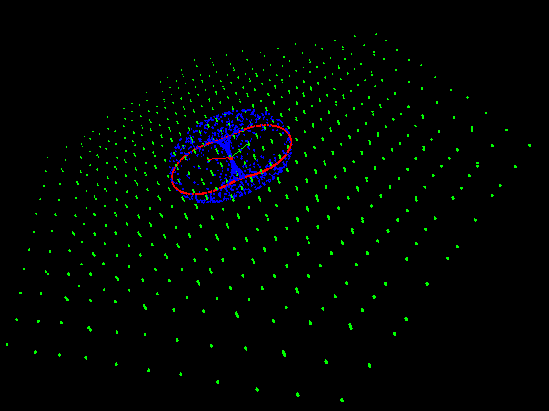
\includegraphics[width=1\linewidth]{pictures/GaalopGradientMethod.png}
    \caption{GradientMethod in Gaalop. Man kann sehen, dass in der Mitte des Torus wesentlich mehr Punkte liegen.}

    \label{fig:GaalopGradientMethod}
\end{figure}
    
\begin{figure}
    \centering
    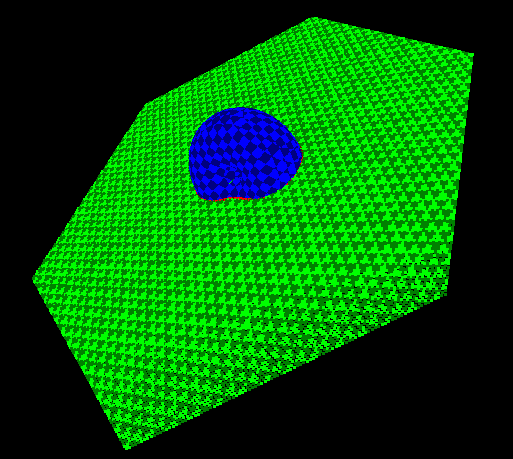
\includegraphics[width=1\linewidth]{pictures/MyGradientMethod.png}
    \caption{GradientMethod in meiner Software mit 100 Abtastpunkten Pro Achse. Die Punktwolke wird so dicht, dass eine Oberfläche entsteht.}

    \label{fig:MyGradientMethod}
\end{figure}
    

\subsection{Grid-basierte Verfahren}
Wie schon gesagt ist TopGrid im Prinzip eine Reimplementierung der Discrete Cube Method aus \textsc{Gaalop}. 
\textsc{Gaalop} hat standartmäßig 100 Abtastpunkten pro Achse und benötigt 8,744 Sekunden ohne Variablen und 57,926 Sekunden mit Variablen.
TopGrid hingegen benötigt bei gleichen Parametern 0,455-0,517 Sekunden, also ca. 20-mal Schneller. Dabei wird ein großer Teil der Zeit damit verbracht die Punkte auf der CPU zu sortieren (profiling sagt ca. 80\%).
Ich finde die Ergebnisse der Methode visuell weder in \textsc{Gaalop}, noch in meiner Implementation besonders überzeugend (siehe \ref{fig:TopGridf}). Trotzdem halte ich die Methode aufgrund ihrer Einfachheit für interessant. 

Die UDF-Approxomation-Variante von TopGrid hingegen liefert wesentlich bessere Ergebnisse (siehe \ref{fig:udfgrid}). Auch der Gauss-Newton Ansatz funktioniert relativ gut, auch wenn es bei Flächen ein paar Ausreißer gibt (siehe \ref{fig:TopGridGN}).
Dabei ist die Auswertung der UDF-Approximation mit 459-504 Sekunden und des Gauss-Newton Ansatzes mit 482-508 Sekunden ungefähr genauso schnell.

Neben TopGrid habe ich außerdem TopGridVoxel implementiert. Dies funktioniert genauso wie TopGrid mit dem Unterschied, dass die Visualisierung als Voxel anstatt als Punktwolke stattfindet.
Die Auswerungsgeschwindigkeit ist mit 0,332-0,406 Sekunden interessanterweise schneller, obwohl bei dieser Methode ein Mesh generiert wird.
Dabei wird etwa jeweils ein Viertel der Zeit für Array Sortierung und Auswertung des Nullraums verbraucht, während die restliche Zeit für die Meshgenerierung gebraucht wird. Das Sortieren ist hierbei schneller, da ich anstatt die Punkte zu sortieren nur den Nullraum sortiere.

Außerdem gibt es noch GridVoxel. Dieses Verfahren implementiert den in \ref{sec:udfvoxel} beschriebenen Ansatz. Da dieser keine Sortierung benötigt, ist er mit 0,254-0,291 Sekunden am schnellsten. Das tolle an diesem Ansatz ist, dass man im Gegensatz zu den TopGrid-Verfahren die Parameter weniger anpassen muss, weshalb es meiner Meinung nach das beste der gitterbasierten Verfahren ist (siehe \ref{fig:GridVoxel}).

\begin{figure}
    \centering
    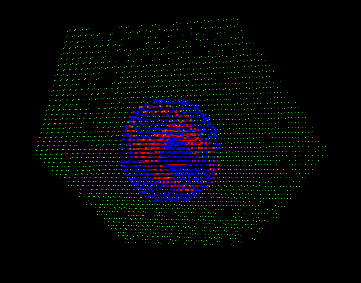
\includegraphics[width=1\linewidth]{pictures/TopGrid.png}
    \caption{TopGrid in meiner Software mit \(f\).}

    \label{fig:TopGridf}
\end{figure}

\begin{figure}
    \centering
    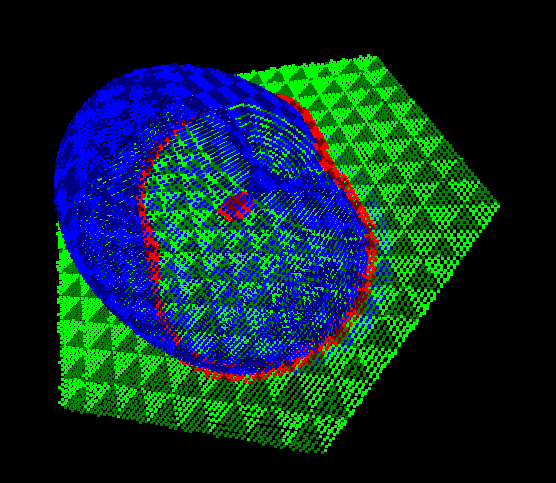
\includegraphics[width=1\linewidth]{pictures/udfgrid.png}
    \caption{TopGrid in meiner Software mit UdfApprox.}

    \label{fig:udfgrid}
\end{figure}

\begin{figure}
    \centering
    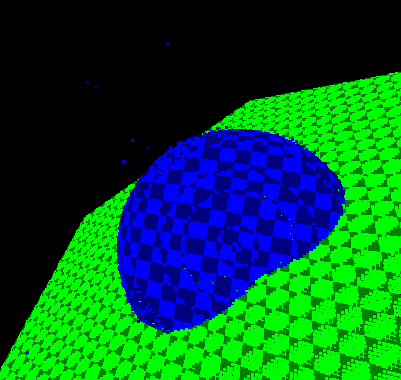
\includegraphics[width=1\linewidth]{pictures/gngrid.png}
    \caption{TopGrid in meiner Software mit Gauss-Newton. Ein paar Ausreißer sind Sichtbar.}

    \label{fig:TopGridGN}
\end{figure}

\begin{figure}
    \centering
    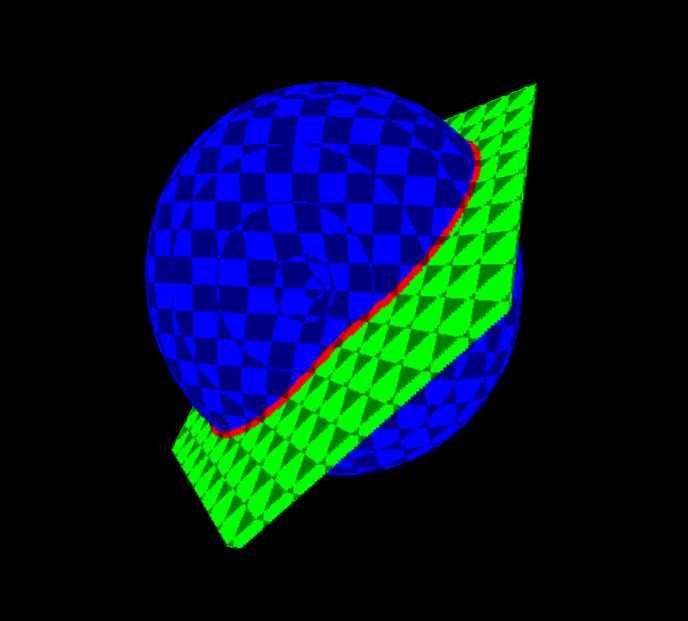
\includegraphics[width=1\linewidth]{pictures/GridVoxel.png}
    \caption{GridVoxel in meiner Software mit einer Auflösung von 200 Abtastpunkten pro Achse. Die voxel sind so klein, dass sie fast nicht mehr sichtbar sind.}

    \label{fig:GridVoxel}
\end{figure}

\subsection{RayMethod Und Intervall Subdivision}
Die RayMethod in \textsc{Gaalop} benutzt Intervallarithmetik, während meine Version das Aberth-Verfahren nutzt. Ich habe auch ein Verfahren, das Intervallarithmetik und Voxel-Subdivision nutzt (Siehe \ref{sec:Voxel-Subdivision}), was aus Sicht der Nullstellensuche ähnlicher ist. Deswegen werde ich das Verfahren mit beiden vergleichen.

Die RayMethod in \textsc{Gaalop} mit Default-Parametern braucht 357,775 Sekunden mit Variablen und 15,607 Sekunden ohne, während mein RayMethod-Verfahren mit vergleichbaren Parametern 0,127-0,150 Sekunden braucht. Das Voxel-Subdivision-Verfahren braucht 0,379-0,445 Sekunden, wobei die Parameter nicht wirklich mit den anderen beiden Verfahren vergleichbar sind.

\textsc{Gaalop}s Verfahren und das Voxel-Subdivision-Verfahren erzeugen sehr dicke Ebenen (Siehe \ref{fig:GaalopRayMethod} und \ref{fig:voxelsubdivision}). Das liegt daran, dass die Intervallarithmetik sehr ungenau ist. Deshalb sind beide Verfahren für Flächen relativ ungeeignet. Meine RayMethod eignet sich hingegen sehr gut für Flächen.
\begin{figure}
    \centering
    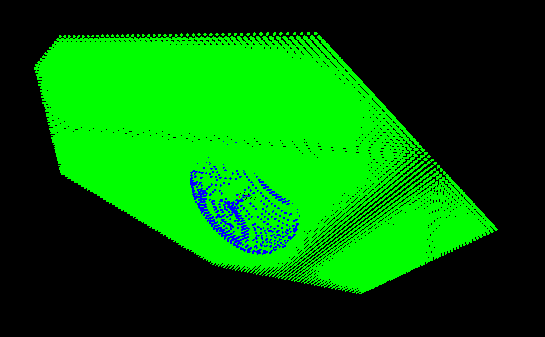
\includegraphics[width=1\linewidth]{pictures/GaalopRayMethod.png}
    \caption{RayMethod in Gaalop. Es werden so viele Punkte generiert, dass die GUI einfriert.}

    \label{fig:GaalopRayMethod}
\end{figure}

\begin{figure}
    \centering
    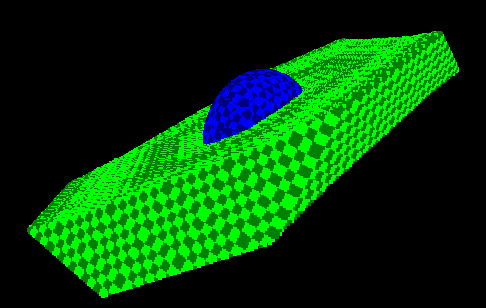
\includegraphics[width=1\linewidth]{pictures/voxelsubdivision.png}
    \caption{VoxelSubdivision in meiner Software. Die Ebene ist sehr dick.}

    \label{fig:voxelsubdivision}
\end{figure}

Eine interessante Eigenschaft meiner RayMethod ist dabei, dass sie im Vergleich zu den gridbasierten Verfahren sehr speichereffizient ist. Der Auswertungs- und Speicheraufwand wächst quadratisch statt kubisch.

Für Kurven sind meine RayMethod und \textsc{Gaalop}s Version schlecht geeignet. Jedoch funktioniert das Intervall-Subdivision-Verfahren gut für Kurven.

Eine interessante Eigenschaft der Subdivision Methode ist, dass sie sehr gut auf verschiedenen Skalen funktioniert. Sie kann sehr kleine Objekte auflösen. Die gitterbasierten oder RayMethod-Verfahren hingegen würden das Objekt verfehlen oder haben eine schlechte Auflösung.

Zusammenfassend lässt sich sagen, dass \textsc{Gaalop}s Version schlechte Ergebnisse für Kurven und Flächen erzeugt und zudem langsam ist. Hingegen ist meine RayMethod sehr schnell und gut für Ebenen geeignet, während die Subdivision-Variante gut für Kurven funktioniert (siehe \ref{fig:rayundsubdivision2}).


\begin{figure}
    \centering
    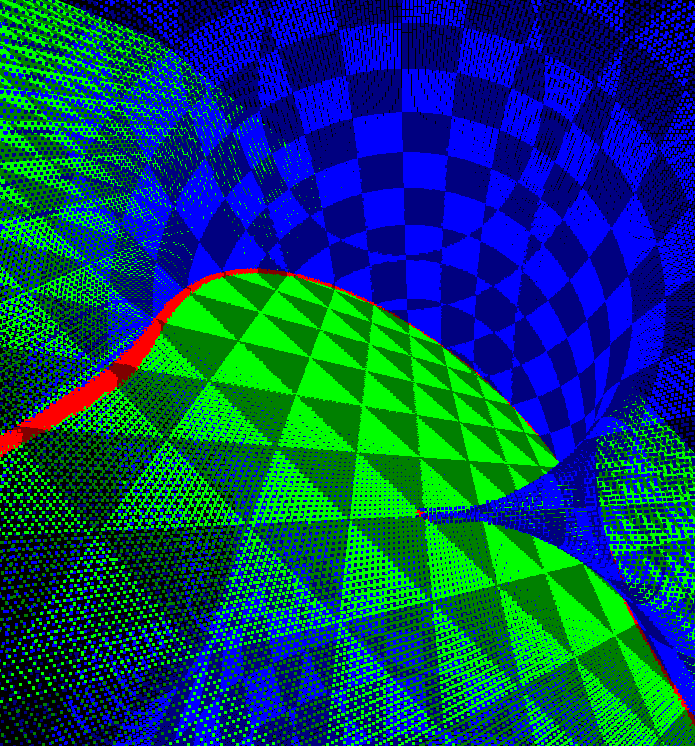
\includegraphics[width=1\linewidth]{pictures/rayundsubdivision2.png}
    \caption{RayMethod für Ebene und Torus und VoxelSubdivision für den Schnitt in meiner Software}

    \label{fig:rayundsubdivision2}
\end{figure}

\subsection{Marching Cubes}
Das Marching-Cubes-Verfahren funktioniert relativ gut. Die Darstellung als Dreiecke statt Punkten ist wesentlich besser. Allerdings gibt es Grenzfälle in denen die Meshgenerierung fehlerhaft ist (Hauptsächlich sieht man Löcher). Das Verfahren hat also gute Ergebnisse allerdings ist es manichmal etwas instabil. Weiterhinn funktioniert das Verfahren nur für Oberflächen und nicht für Kurven (siehe \ref{fig:MC}). Außerdem visualisiert das Verfahren eher lokale Minima statt Nullstellen. Ich habe in meinen Beispielen keine Unterschiede festgestellt, allerdings könnte dies Probleme verursachen. 


\begin{figure}
    \centering
    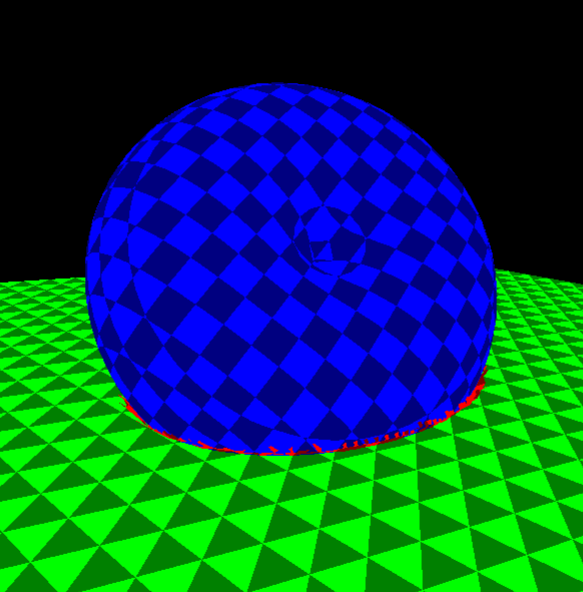
\includegraphics[width=1\linewidth]{pictures/MC.png}
    \caption{Marching Cubes in meiner Software. Die Geometrie ist schön und schnell, allerdings funktioniert das Verfahren nicht für Kurven.}

    \label{fig:MC}
\end{figure}


\section{Raycasting}
In diese Sektion werde ich die Raycasting-Ansätze untersuchen. Dabei habe ich mich teilweise für eine ein bischen andere Szene entschieden um Artefakte besser darstellen zu können.
Der Fokus liegt dabei auf den visuallen Artefakten der Verfahren.
%Stabilität (wie wichtig ist hyperparameter tuning)
%Performance
%TODO
\subsection{UdfApprox und Newton}
Bei diesen Verfahren gibt es drei Möglichkeiten für fehlerhafte Darstellung. Entweder wird ein zu großer Schritt gemacht und die Nullstelle wird übersprungen, oder es werden zu kleine Schritte gemacht und die Nullstelle wird nie erreicht, oder das Verfahren denkt, es habe eine Nullstelle gefunden, obwohl dies nicht der Fall ist.

Dabei hat das UdfApprox-Verfahren in der Regel das Problem, dass es nicht konvergiert, wobei das Newtonverfahren Nullstellen überspringt. Dies hängt unter anderem damit zusammen ,dass ein Schritt des Newtonverfahrens stets größer als ein Schritt der UDF-Approximation ist (siehe \ref{fig:newton}).
\begin{figure}
    \centering
    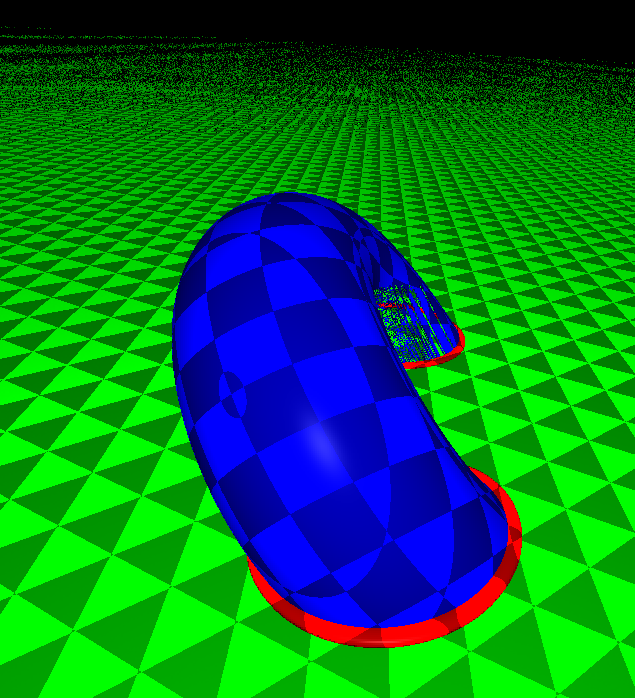
\includegraphics[width=1\linewidth]{pictures/newton.png}
    \caption{Newton konvergiert in größeren Entfernungen als UdfApprox, hat aber mehr Artefakte.}

    \label{fig:newton}
\end{figure}

Dabei konvergiert das UdfApprox-Verfahren vor allem bei flachen Ebenen schlecht, was ein allgemeines Problem von Spheretracing ist (siehe \ref{fig:udfapprox}). 
\begin{figure}
    \centering
    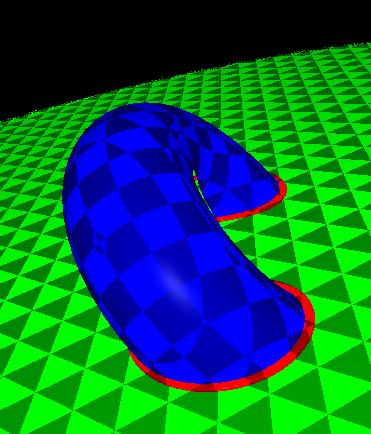
\includegraphics[width=1\linewidth]{pictures/udfaprox.png}
    \caption{Hier kann man sehen, dass das UdfApprox-Verfahren für die Ebene am Horizont nicht konvergiert, und auch der Torus hat ein Loch.}

    \label{fig:udfapprox}
\end{figure}

Beide Verfahren können vor allem bei lokalen Maxima des Nullraums, an denen die Ableitung null ist, explodieren. Dabei passiert dies beim Newtonverfahren wesentlich häufiger, da es bei den lokalen Maxima des Raycasting-Strahls explodiert, während die UDF-Approximation nur bei den lokalen Maxima des Raums explodiert. Dem wird duch eine kleinere maximale Schrittweite entgegengewirkt. (siehe \ref{fig:torusvoninnen} und \ref{fig:torusudfapprox})

\begin{figure}
    \centering
    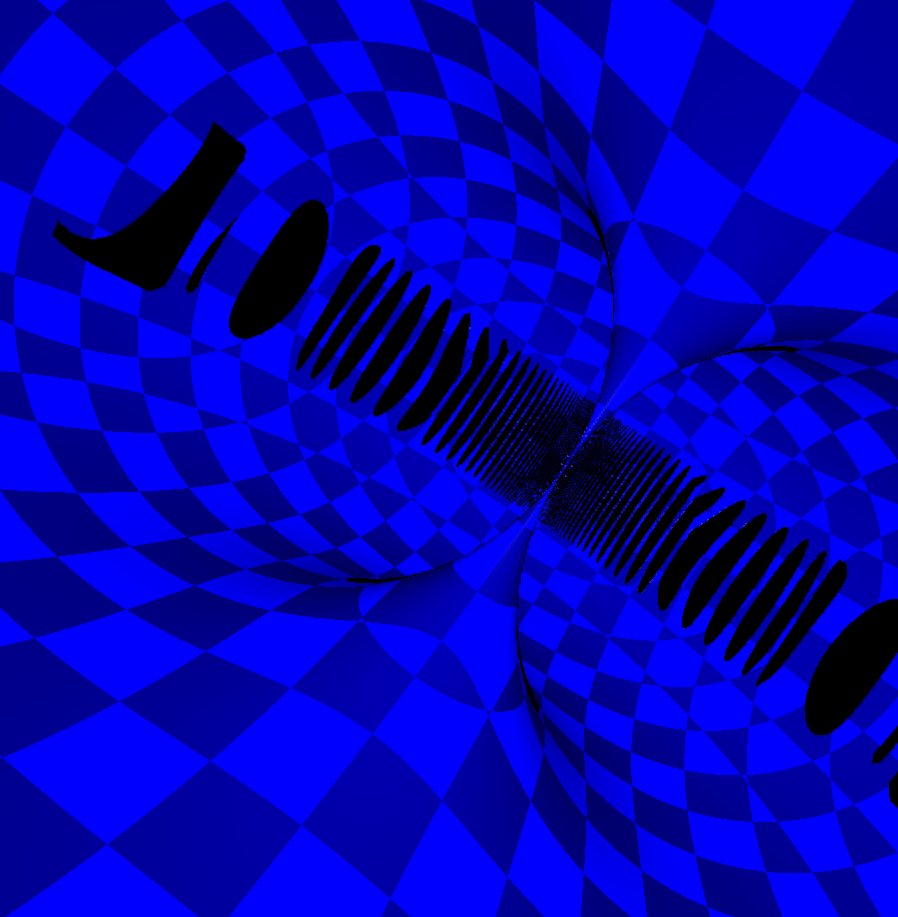
\includegraphics[width=1\linewidth]{pictures/torusvoninnen.png}
    \caption{Torus von innen mit UdfApprox. Ein lokales Maximum liegt in der Mitte des Rings des Torus und die Verfahren überspringen die Nullstelle.}

    \label{fig:torusvoninnen}
\end{figure}

\begin{figure}
    \centering
    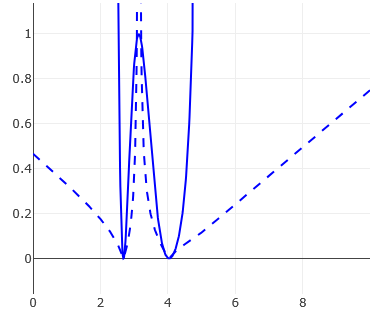
\includegraphics[width=1\linewidth]{pictures/torusudfaprox.png}
    \caption{\(f_\text{ray}\) des Torus und die UDF-Approximation (gestrichelt) entlang eines Strahls durch ein lokales Maximum. Das Maximum in diesem Fall liegt in der Mitte des Rings des Torus. An dieser Stelle explodiert die UDF-Approximation. }

    \label{fig:torusudfapprox}
\end{figure}

Die UDF-Approximation eignet sich besonders gut zum Rendern von Kurven. Das liegt daran, dass Kurven als Röhren gerendert werden. Die Dicke der Röhre lässt sich dabei über den Schwellwert einstellen. Das Newtonverfahren ist schlechter zum Kurvenrendern geeignet, da die Kurven in der Regel flach sind. Außerdem kann sich die Form der Kurve beim Newtonverfahren mit Änderung des Blickwinkels verändern.

Das Newtonverfahren ist ein bisschen schneller mit ca. 25 FPS und die UDF-Approximation ein bisschen langsamer mit ca. 20 FPS.
Das Tile-Rendering braucht für die UDF-Approximation ca. 1,3 Sekunden und für das Newtonverfahren ca. 1,1 Sekunde. Dabei haben die Bilder in Bewegung ein Fünftel der Auflösung in beide Richtungen.
Deshalb ist der Aufwand für das volle Bild ca. 25-mal so groß. Das bedeutet, dass der Tile rendering overhead relativ klein ist.
Das Tile rendering rendert Tiles mit immer einem Tile pro Frame. Bei meiner aktuellen Bildschirmauflösung werden 32 Tiles gerendert, was bedeutet, dass das Tilerendering immer mindestens 0,53 Sekunden braucht.










\subsection{Aberth}
Das Aberth-Verfahren findet die imaginären Nullstellen eines Teilpolynoms und versucht dann herauszufinden, ob die imaginären Nullstellen echte Nullstellen sind. Dazu wird die UDF-Approximation benutzt.

Im Vergleich zu den anderen Verfahren hat dieses Verfahren wenige Artefakte und ist relativ stabil. Artefakte entstehen hauptsächlich dadurch, dass die imaginären Nullstellen fehlerhafterweise visualisiert werden (siehe \ref{fig:aberthbad}).
\begin{figure}
    \centering
    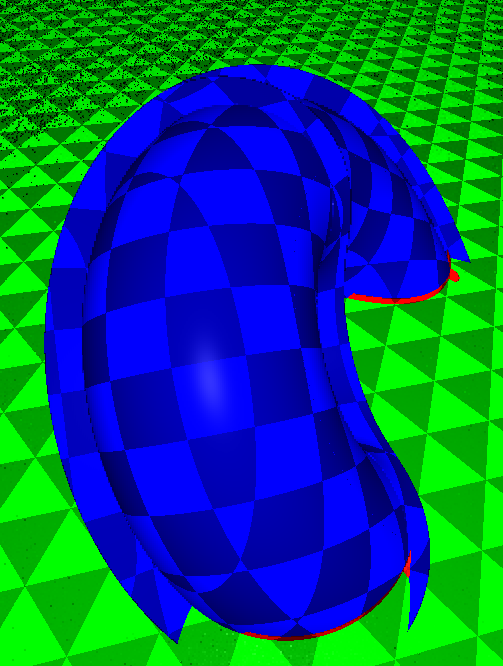
\includegraphics[width=1\linewidth]{pictures/aberthbad.png}
    \caption{Aberth-Verfahren mit zu groß gewähltem Schwellwert. Man kann sehen, wie die imaginären Nullstellen in der Nähe des Torus fehlerhaft dargestellt werden.}

    \label{fig:aberthbad}
\end{figure}

Im Gegensatz zur UDF-Approximation ist das Verfahren nur schlecht geeignet, um Kurven darzustellen. Das liegt daran, dass ein größerer Schwellwert bedeutet, dass die imaginären Nullstellen verstärkt dargestellt werden, was mehr Artefakte verursacht. Ein kleiner Schwellwert funktioniert, allerdings sind die Kurven dann sehr dünn (siehe \ref{fig:aberth}).

Im Vergleich zum Newton Verfahren ist das Aberth Verfahren Visuell eigentlich immer besser da es für Flächen weniger Artefakte hat. Allerdings kann es sein, dass für eine gute darstellung die Parameter etwas angepasst werden müssen.

Das Aberth-Verfahren hat relativ hochfrequentes Rauschen auf den gefundenen Nullstellen. Deshalb habe ich mich entschieden, die aufwendigere Methode zur Normalenberechnung anhand der Ableitung des Nullraums zu implementieren.

Das Aberth-Verfahren hat auch etwa 25 FPS. In der aktuellen Aberth-Variante berechne ich erst 20 Iterationen des Aberth-Verfahrens mit angenäherten Koeffizienten, und dann nochmal 20 Iterationen des Aberth-Verfahrens mit der originalen Funktion.
Wenn man stattdessen 40 Iterationen der original Funktion und keine Iterationen der angenäherten Funktion berechnet, hat das Verfahren nur 15 FPS.


Neben dem Aberth-Verfahren gibt es auch noch AberthGN. Ich konnte keine visuellen Unterschiede zwischen den Verfahren feststellen. Da Gauss-Newton bei den gridbasierten Verfahren für Flächen jedoch zu Ausreißern neigt, ist es potenziell instabiler. Deshalb habe ich es aus der GUI rausgenommen. Für Kurven könnte dieser Ansatz theoretisch stabiler sein, allerdings ist das Aberth-Verfahren für Kurven sowieso ungeeignet.

\begin{figure}
    \centering
    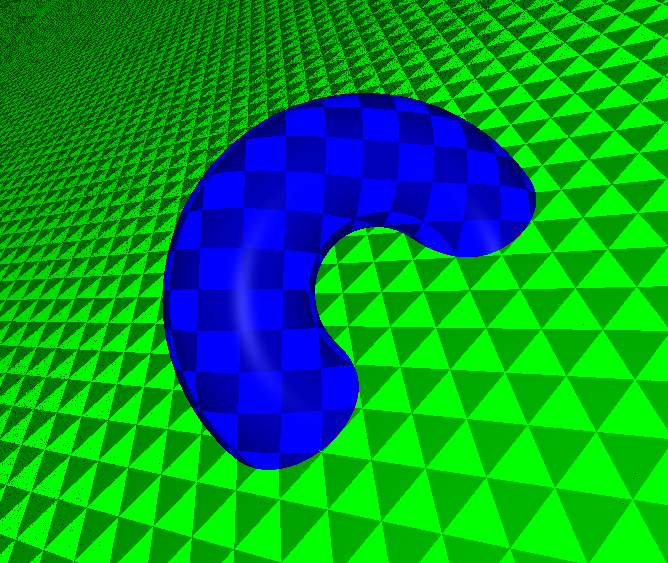
\includegraphics[width=1\linewidth]{pictures/aberth.png}
    \caption{Aberth-Verfahren mit Default-Parametern. Die Kurve ist so dünn, dass sie fast unsichtbar ist.}

    \label{fig:aberth}
\end{figure}


\subsection{Instabilität bei doppelten Nullstellen}
Alle meine Raycasting-Verfahren haben ein Problem, die grüne Ebene darzustellen (\ref{fig:doubleroot_plane}). Das liegt daran, dass die Ebene eine doppelte Nullstelle hat. Dies macht leider alle meine Verfahren instabil. Das Aberth-Verfahren kann nach dem Konvergieren explodieren (siehe \ref{fig:doubleroot_complexplane}), und auch die UDF-Approximation explodiert (siehe \ref{fig:doubleroot_alongray}). Dies ist ein allgemeines Problem vieler Verfahren zur polynomiellen Nullstellensuche. In der Regel wird ein sogenanntes square-free Polynom berechnet. Allerdings ist dies relativ aufwendig.
\begin{figure}
    \centering
    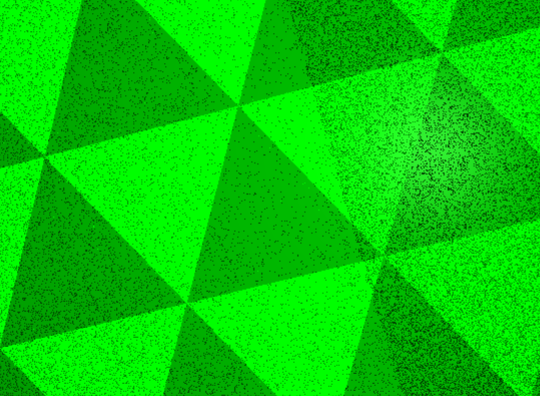
\includegraphics[width=1\linewidth]{pictures/doubleroot.png}
    \caption{Ebene visualisiert mit Aberth aus der Nähe. An den schwarzen Pixeln konvergiert das Verfahren nicht. In der Regel wird das Muster schlechter, desto weiter man vom Ursprung entfernt ist. Ich vermute, dass liegt an schlechter Gleitkommapräzision. }

    \label{fig:doubleroot_plane}
\end{figure}
\begin{figure}
    \centering
    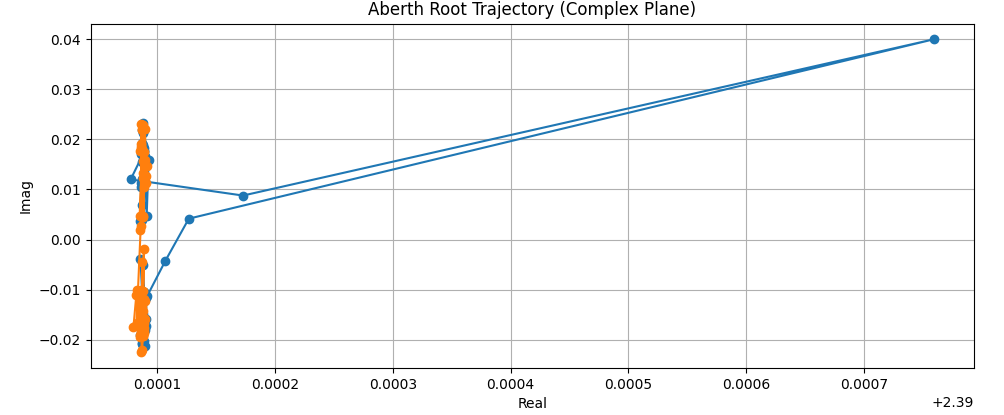
\includegraphics[width=1\linewidth]{pictures/doubleroot_rootconvergence.png}
    \caption{Darstellung der komplexen Nullstellen des Aberth-Verfahrens über mehrere Iterationen. Hier sieht man wie die komplexen Nullstellen plötzlich explodieren können. }

    \label{fig:doubleroot_complexplane}
\end{figure}

\begin{figure}
    \centering
    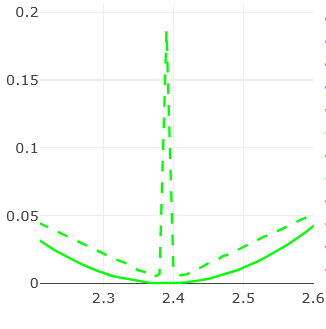
\includegraphics[width=1\linewidth]{pictures/doubleroot_alongray.png}
    \caption{UdfApprox (gestrichelt) und \((\mathbf{F}_R(\mathbf{ray}(a)))_1\) entlang eines Strahls. Die UDF-Approximation explodiert an der Nullstelle. }

    \label{fig:doubleroot_alongray}
\end{figure}
\subsection{Ganja}
Wie schon beschrieben nutzt Ganja Sphere Tracing mit \(\sqrt{f_\text{ray}(t)}\)
als Distanzfunktion. Das Hauptproblem ist, dass dieses Verfahren sehr instabil für hochdimensionale Algebren ist. Ich musste viel mit Parametern herumprobieren, bis überhaupt ein sichtbares Bild entsteht, und bei falschen Parametern verschwindet das Objekt einfach. Und auch dann sind Objekte nur in der Nähe der Kamera sichtbar. Bei meinen Verfahren verschwindet das Objekt auch bei schlechten Parametern, allerdings ist Ganja wesentlich empfindlicher.

Ein weiteres Problem ist, dass sich Objekte verändern, wenn sie mit einem Skalar multipliziert werden. Wenn ein Multivektor mit einem Skalar multipliziert wird, wird auch der zugehörige Nullraum des Multivektors entsprechend skaliert. Da die Nullstellen durch die Skalierung an der gleichen Stelle bleiben, dürfte sich das Objekt nicht ändern, bei Ganja verändert sich jedoch die Visualisierung. Ich habe Ganjas Verfahren in meiner Software nachimplementiert, allerdings habe ich wie bei den anderen Verfahren auch eine maximale Schrittweite hinzugefügt, was das Verfahren wesentlich stabiler macht.

Ein weiteres Problem von Ganja in hochdimensionalen Algebren ist, dass der generierte Code für Kurven teilweise zu groß ist. Das liegt daran, dass Ganja nicht wie in meinem Ansatz eine QR-Zerlegung nutzt, um die Codegröße auf der GPU zu beschränken. Deshalb konnte ich die Visualisierung von Kurven nicht in Ganja testen. Der Code hat sich für mehrere Minuten beim Kompilieren des Shaders aufgehängt, und danach war keine Kurve sichtbar. Ich bin nicht sicher, ob dies an schlecht gewählten Parametern liegt oder ob OpenGL aufgegeben hat.

Ein Vorteil von Ganjas Visualisierung ist, dass der generierte Shader-Code relativ schnell kompiliert und (bis auf Kurven) schneller als meine Verfahren ist. Das liegt daran, dass meine aktuelle Codegenerierung immer eine QR-Zerlegung nutzt, nicht nur, wenn das Gleichungssystem überdeterminiert ist, und dann später einfach Nullen hochlädt. Im Prinzip bedeutet das, dass Ganja im Best Case schneller ist, während meine Software im Worst Case schneller ist.

Die Performancemessung in Ganja ist ein bisschen komplizierter, da Ganja keine direkte eingebaute Zeitmessung hat.
Ganjas Visualisierung braucht ca. 8 ms bis 400 ms pro Animation-Loop-Durchlauf mit durchschnittlich ca. 175 ms. Wenn man annimmt, dass in jedem Durchlauf ein Frame mit voller Auflösung gerendert wird, entspricht das ca. 6 FPS. Dies ist wesentlich schneller als das Tile-Rendering in meinem Ansatz. Allerdings ist die Reaktionszeit von Ganja größer, da es kein Tile-Rendering nutzt.

\begin{figure}
    \centering
    
\includegraphics[width=1\linewidth]{pictures/ganjadcga.png}
    \caption{Die Beispielszene in Ganja. Aus anderen Blickwinkeln verschwindet der Torus teilweise.}

    \label{fig:ganjadcga}
\end{figure}
\begin{figure}
    \centering
    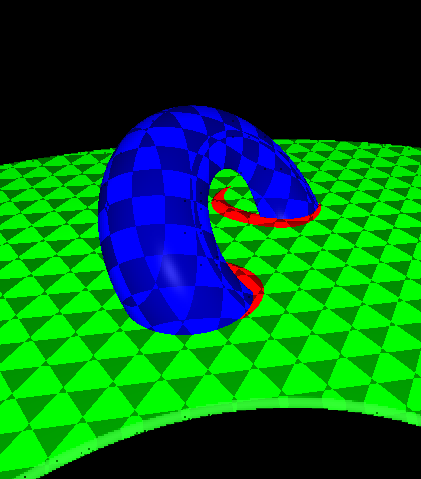
\includegraphics[width=1\linewidth]{pictures/myganja.png}
    \caption{Die Beispielszene in meiner Version von Ganjas Verfahren. Ganjas Ansatz hat viele Artefakte.}

    \label{fig:myganja}
\end{figure}

\section{Weitere Beispiele}
Um die Software auszuführen, muss ein Webserver bereitgestellt werden. Falls Python installiert ist, kann dieser mit der \texttt{server.bat} gestartet werden. Die Software ist dann im Browser unter \url{http://localhost/} erreichbar.

Ein paar Beispiele befinden sich im Ordner \texttt{jsgaalop\textbackslash assets\textbackslash examples2}. Die kompilierten JSON-Dateien liegen im Unterordner \texttt{compiled}.

Die \texttt{compile.bat} kompiliert alle Beispiele im Unterordner \texttt{input}. Dabei wird der Kommentar in der ersten Zeile als Command-Line-Argument an GAALOP übergeben. Mit der Option \texttt{-a} kann die Algebra angegeben werden.

Damit \texttt{compile.bat} GAALOP ausführen kann, muss Java installiert sein. Eine kompilierte GAALOP-Version mit dem Plugin befindet sich unter \texttt{jsgaalop\textbackslash assets\textbackslash distribution-2.2.6.2-bin}.

\begin{figure}
    \centering
    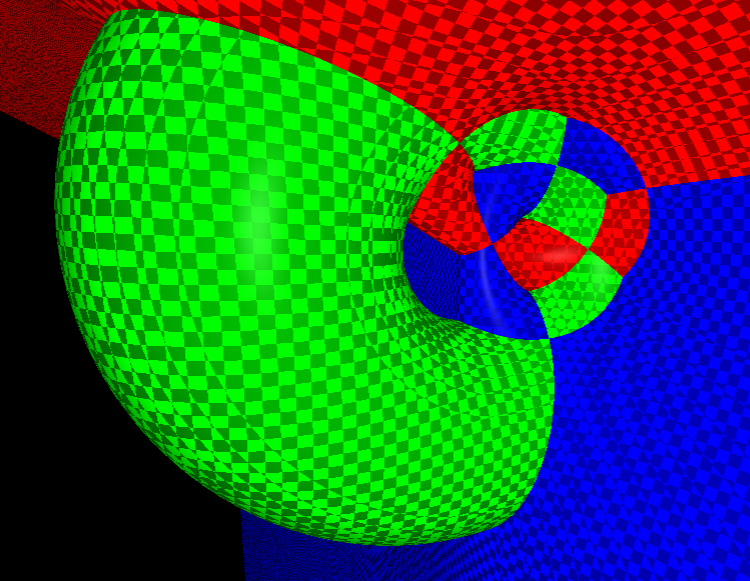
\includegraphics[width=1\linewidth]{pictures/P123.png}
    \caption{Visualisierung der Torus Inversion von Seite 123 aus \cite{hildenbrand2021power}.}

    \label{fig:P123}
\end{figure}



\begin{figure}
    \centering
    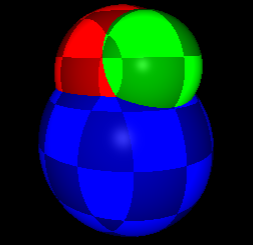
\includegraphics[width=1\linewidth]{pictures/threesperes.png}
    \caption{Visualisierung des Three-Spheres-Beispiels von Seite 66 aus \cite{hildenbrand2021power}. Dieses Beispiel kann auch mittels Ganja unter folgendem Link visualisiert werden: \href{https://gaalopweb.esa.informatik.tu-darmstadt.de/gaalopweb/res/cpp/input?sample=threespheres}{Online-Visualisierung}}

    \label{fig:threesperes}
\end{figure}

\begin{figure}
    \centering
    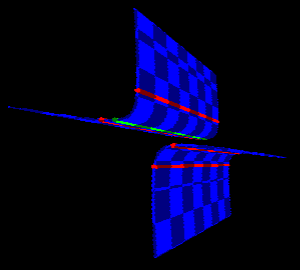
\includegraphics[width=1\linewidth]{pictures/P93.png}
    \caption{Dieses Beispiel ist eigentlich 2d, wird in meiner Software aber als 3d dargestellt. (aus Seite 93 aus \cite{hildenbrand2021power})}

    \label{fig:threesperes}
\end{figure}

\chapter{Zusammenfassung}
Das Ziel der Arbeit war es eine performante Visualisierung für \textsc{Gaalop}Web zu entwickeln, die mit hochdimensionaler Algebra umgehen kann.

Dazu wurde ein Verfahren entwickelt, welches Shadercode zur Evaluierung des Nullraums von geometrischen Objekten erzeugt. Anders als Ganjas Ansatz funktioniert mein Ansatz auch in hochdimensionalen Algebren. Dabei wird mittels QR-Zerlegung die Größe des generierten Shadercodes reduziert, was die Auswertung in hochdimensionalen Algebren erst ermöglicht.

Darauf aufbauend wurden neue Visualisierungsmethoden entwickelt, die auf den Ansätzen von Gaalop und Ganja aufbauen.

Der Vorteil meiner Ansätze gegenüber Gaalop ist, dass die Evaluierung wesentlich schneller ist. Je nach Anwendungsfall zwischen 20-mal und 2000-mal. Dies bedeutet unter anderem, dass Objekte in wesentlich höherer Auflösung visualisiert werden können. Außerdem erzeugen meine Ansätze im Gegensatz zu Gaalop unter anderem einfache Meshes anstatt nur Punktwolken.
Von den volumenbasierten Ansätzen empfehle ich GridVoxel als stabiles Verfahren zur Meshgenerierung (Dieser Ansatz ist hauptsächlich bei hohen Auflösungen interessant), RayMethod als schnelles Verfahren zur Punktwolkengenerierung von Flächen, IterGrid zur Punktwolkengenerierung von Kurven und Marching Cubes als ein etwas instabileres Verfahren, welches komplexere Meshes erzeugen kann.


Die auf Ganja aufbauenden Raycasting-Verfahren sind hingegen wesentlich stabiler als Ganjas eigenes Verfahren und haben weniger Artefakte.
Von den Raycasting-Verfahren empfehle ich UdfApprox für Kurven und Aberth für Flächen. 
Ein bekanntes Problem meiner Raycasting-Verfahren ist die Instabilität bei doppelten Nullstellen im Nullraum, was zu Artefakten bei der Darstellung von Ebenen in der DCGA führt.

Insgesamt zeigen die Ergebnisse, dass die entwickelten Methoden die Anforderungen an Geschwindigkeit und Qualität erfüllen.

\chapter{Ausblick}
Der wichtigste nächste Schritt wäre die Integration der Software in \textsc{Gaalop}Web. Die Software ist dafür vorbereitet, und die Integration müsste relativ einfach sein. Da ich keinen Zugriff auf den source Code von \textsc{Gaalop}Web habe, konnte ich dies nicht selbst machen.

Außerdem könnte man versuchen, das Problem zu lösen, auf welches ich bei meinen Raycasting-Ansätzen gestoßen bin. Im Prinzip bedeutet das, einen stabilen Algorithmus zu finden, der auf der GPU reelle Nullstellen von Polynomen mit doppelten Nullstellen finden kann. Außerdem wird ein Algorithmus benötigt, der feststellen kann ob sich an einem Punkt (oder in der Nähe) eine Reelle nullstelle befindet.

Ein weiterer wichtiger Punkt währe die überargeitung der GUI.
Aktuell hat die Software viele Parameter und Visualisierungsansätze mit vielen Hyperparametern. In der Praxis werden wahrscheinlich nur wenige dieser Methoden sinnvoll sein. Deshalb wäre einer der nächsten Schritte, viele Methoden zu entfernen oder zu verstecken. Das Gleiche gilt für die Parameter in der GUI. Außerdem kann das Diagramm, welches ich zum Debugging eingefügt hatte, entfernt werden.

Eine weitere Verbesserung wäre eine bessere Codegenerierung. Dazu gehört eine Untersuchung der alten und neuen Codegenerierung für schnelle Ableitungsberechnung. Als Nächstes könnte man die Multiplikation mit der Matrix \(R\) in GLSL verbessern, falls \(R\) keinen vollen Rang hat. Im Moment wird mit der gesamten Matrix \(R\) multipliziert, obwohl \(R\) Zeilen mit Nullen hat. Alternativ könnte man statt für jedes Objekt einen einzelnen Shader zu kompilieren, einen Shader pro Algebra kompilieren. Dies könnte die Visualisierung einfacher machen, da die Shader nicht für jedes Objekt neu kompiliert werden müssen.


\printbibliography



\end{document}
%% End of file `DEMO-TUDaThesis.tex'.
